% +++
% latex="texfot lualatex-dev"
% +++
\documentclass[body]{subfiles}
\begin{document}
\chapter{実験結果}

\section{計算結果が平衡状態であるか}

各実験での全球平均外向き赤外放射 (OLR) と全球平均入射短波放射 (OSR) の
全球平均の時系列図を図 \ref{OLR-OSRA} に示す。この図を見ると、 S1366
から S1800 の太陽定数では、 おおよそ 10 年以上積分をすることで、全球平均
OLR と OSR がほぼ一致して、大気の状態が平衡になっていることがわかる。
一方で、S2000 では、全球平均 OLR が激しく変動していて、この図からは平衡
状態に達しているかは判断できない。

次に、各実験での OLR の東西平均を図 \ref{OLR東西平均} に、地表面温度の
東西平均を図 \ref{地表面温度} に示す。この図を見ると、灰色大気・雲なしの
モデルで Ishiwatari \etal (2002) が結論したように、非灰色大気・雲ありの
モデルでも、太陽定数が増大したときに、OLR の南北分布が一様になることが見て取れる。

\begin{figure}[t]
	\centering
	\begin{subfigure}{.4\textwidth}
		\centering
		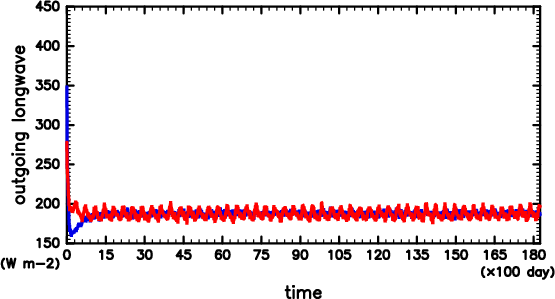
\includegraphics[width=\columnwidth]{S1366/S1366_OLRA-OSRA_horimean_time0.0-18250.0-crop.png}
		\caption{\(S=1366\hmu{W/m^2}\)}
	\end{subfigure}
	\begin{subfigure}{.4\textwidth}
		\centering
		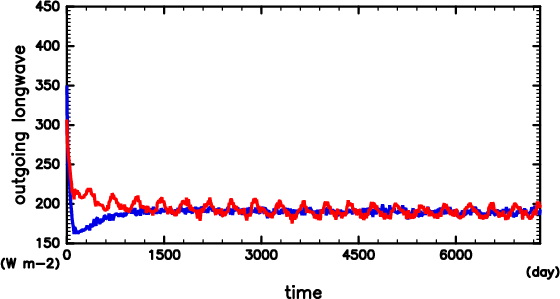
\includegraphics[width=\columnwidth]{S1500/S1500_OLRA-OSRA_horimean_time0.0-7300.0-crop.png}
		\caption{\(S=1500\hmu{W/m^2}\)}
	\end{subfigure}
	\begin{subfigure}{.4\textwidth}
		\centering
		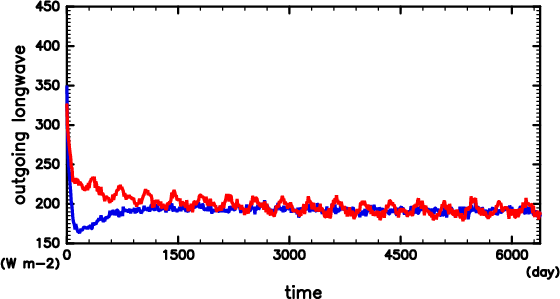
\includegraphics[width=\columnwidth]{S1600/S1600_OLRA-OSRA_horimean_time0.0-7300.0-crop.png}
		\caption{\(S=1600\hmu{W/m^2}\)}
	\end{subfigure}
	\begin{subfigure}{.4\textwidth}
		\centering
		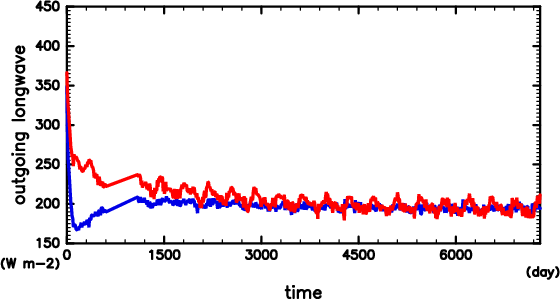
\includegraphics[width=\columnwidth]{S1800/S1800_OLRA-OSRA_horimean_time0.0-7300.0-crop.png}
		\caption{\(S=1800\hmu{W/m^2}\)}
	\end{subfigure}
	\begin{subfigure}{.4\textwidth}
		\centering
		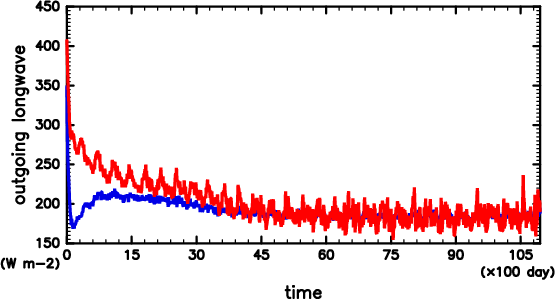
\includegraphics[width=\columnwidth]{S2000/S2000_OLRA-OSRA_horimean_time0.0-10950.0-crop.png}
		\caption{\(S=2000\hmu{W/m^2}\)}
	\end{subfigure}
	\caption{各実験での全球平均した OLR(赤線)と OSR(青線)の時系列変化}\label{OLR-OSR}
\end{figure}

\begin{figure}[t]
	\centering
	\begin{minipage}{.45\textwidth}
		\centering
		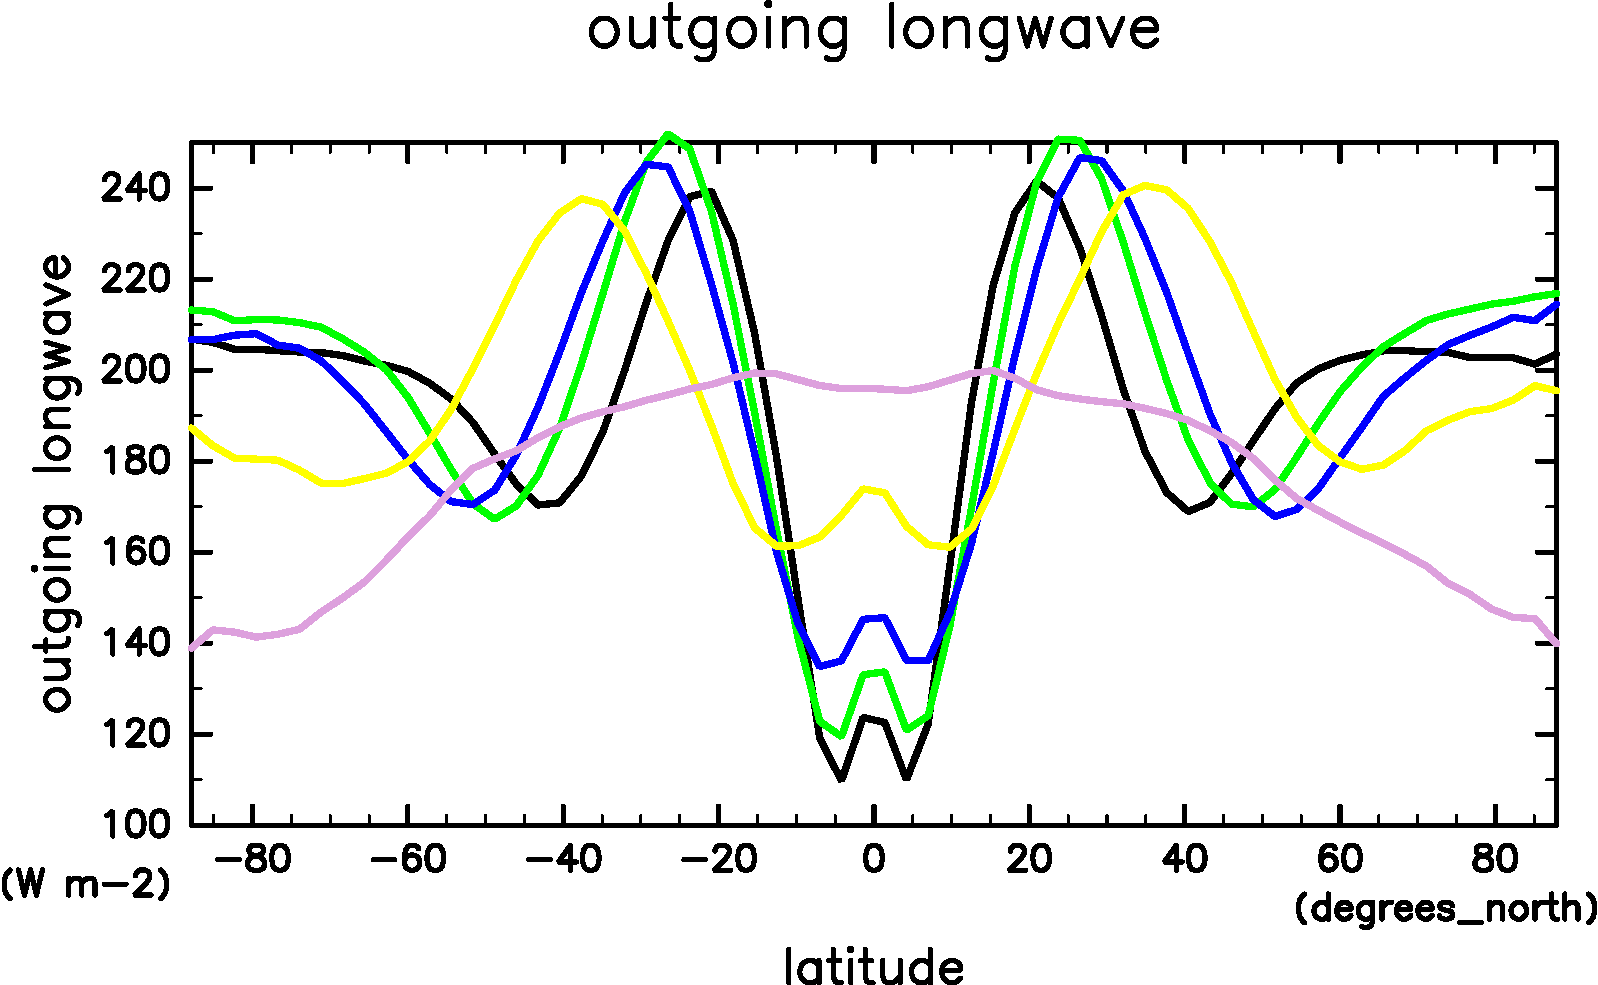
\includegraphics[width=\textwidth]{OLR-overplot-crop-rotate.pdf}
		\caption[各実験での OLR の東西平均]{
			各実験での OLR の東西平均。それぞれ、黒線: S1366;
			緑線: S1500; 青線: S1600; 黄線: S1800; 桃線: S2000 の結果である。
		}\label{OLR東西平均}
	\end{minipage}
	\hfill
	\begin{minipage}{.45\textwidth}
		\centering
		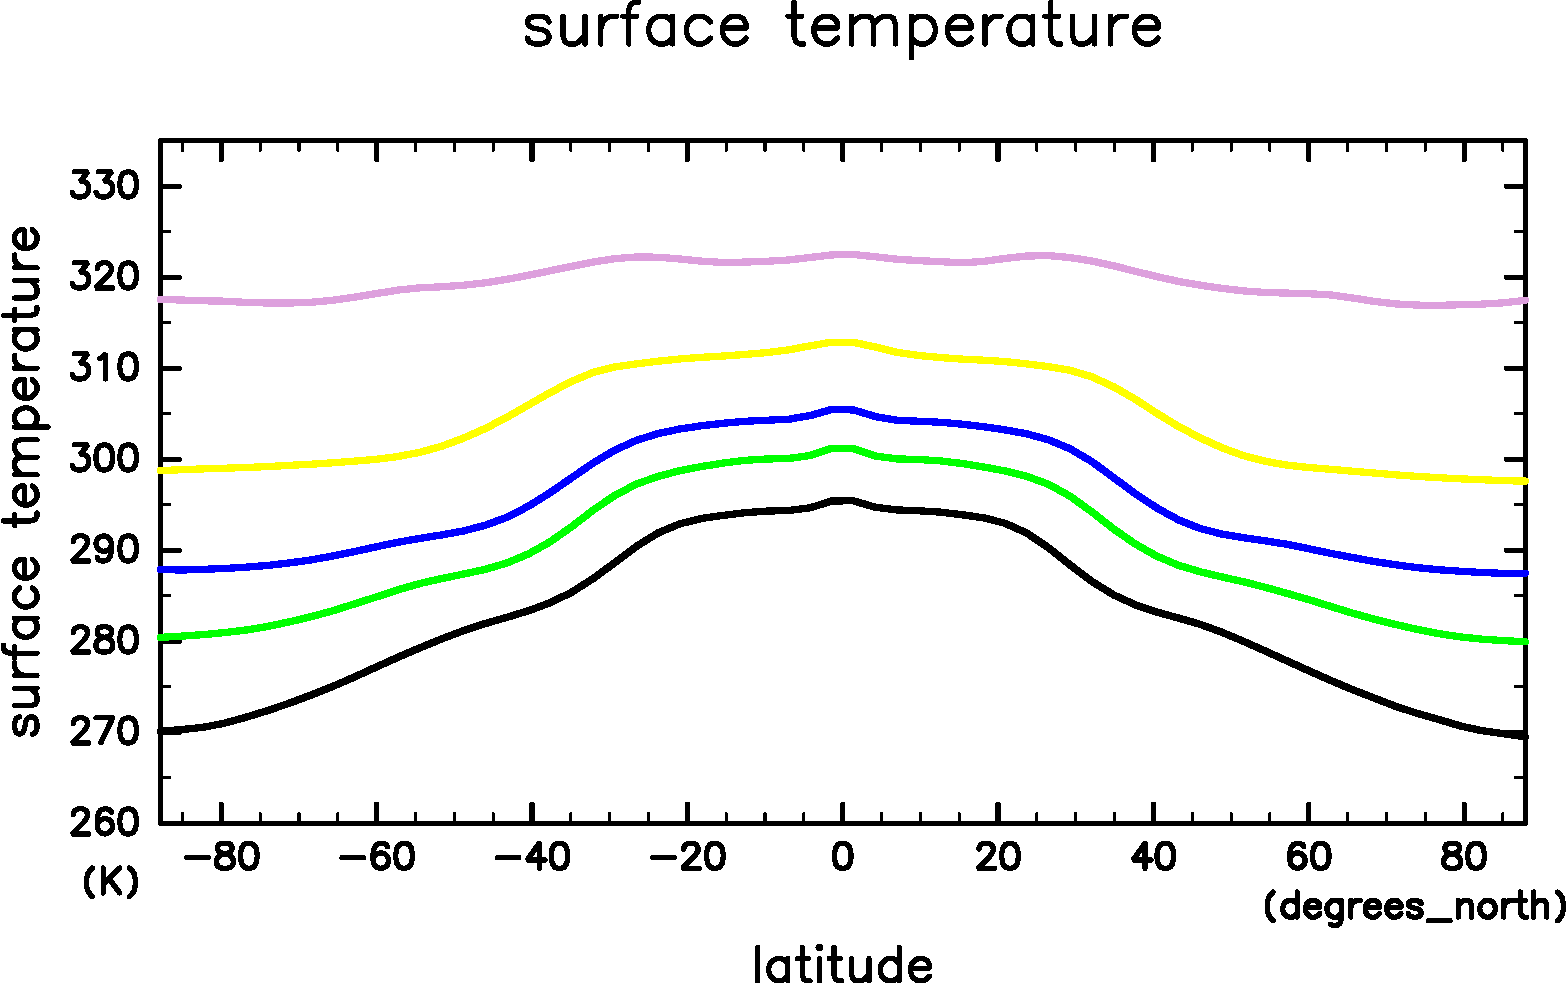
\includegraphics[width=\textwidth]{SurfTemp-overplot-crop-rotate.pdf}
		\caption[各実験での地表面温度の東西平均]{
			各実験での地表面温度の東西平均。それぞれ、黒線: S1366;
			緑線: S1500; 青線: S1600; 黄線: S1800; 桃線: S2000 の結果である。
		}\label{地表面温度}
	\end{minipage}
\end{figure}

\begin{figure}[t]
	\centering
	\begin{subfigure}{.4\textwidth}
		\centering
		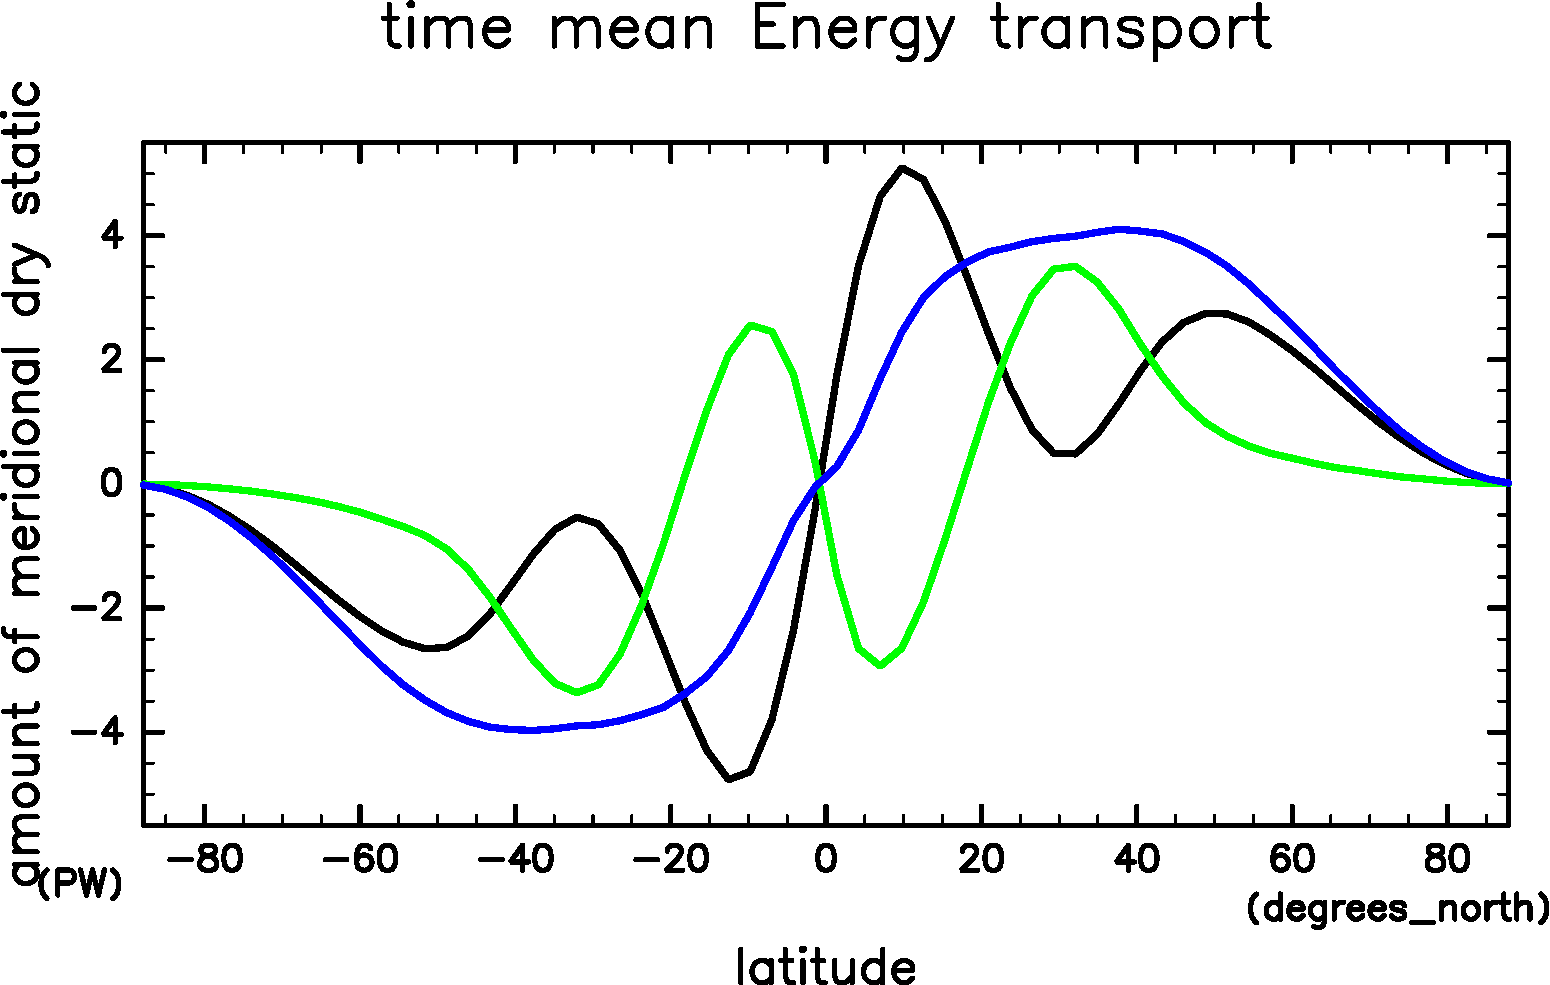
\includegraphics[width=\columnwidth]{S1366/EngyFlx,time=14600:14965-crop-rotate.pdf}
		\caption{\(S=1366\hmu{W/m^2}\)}
	\end{subfigure}
	\begin{subfigure}{.4\textwidth}
		\centering
		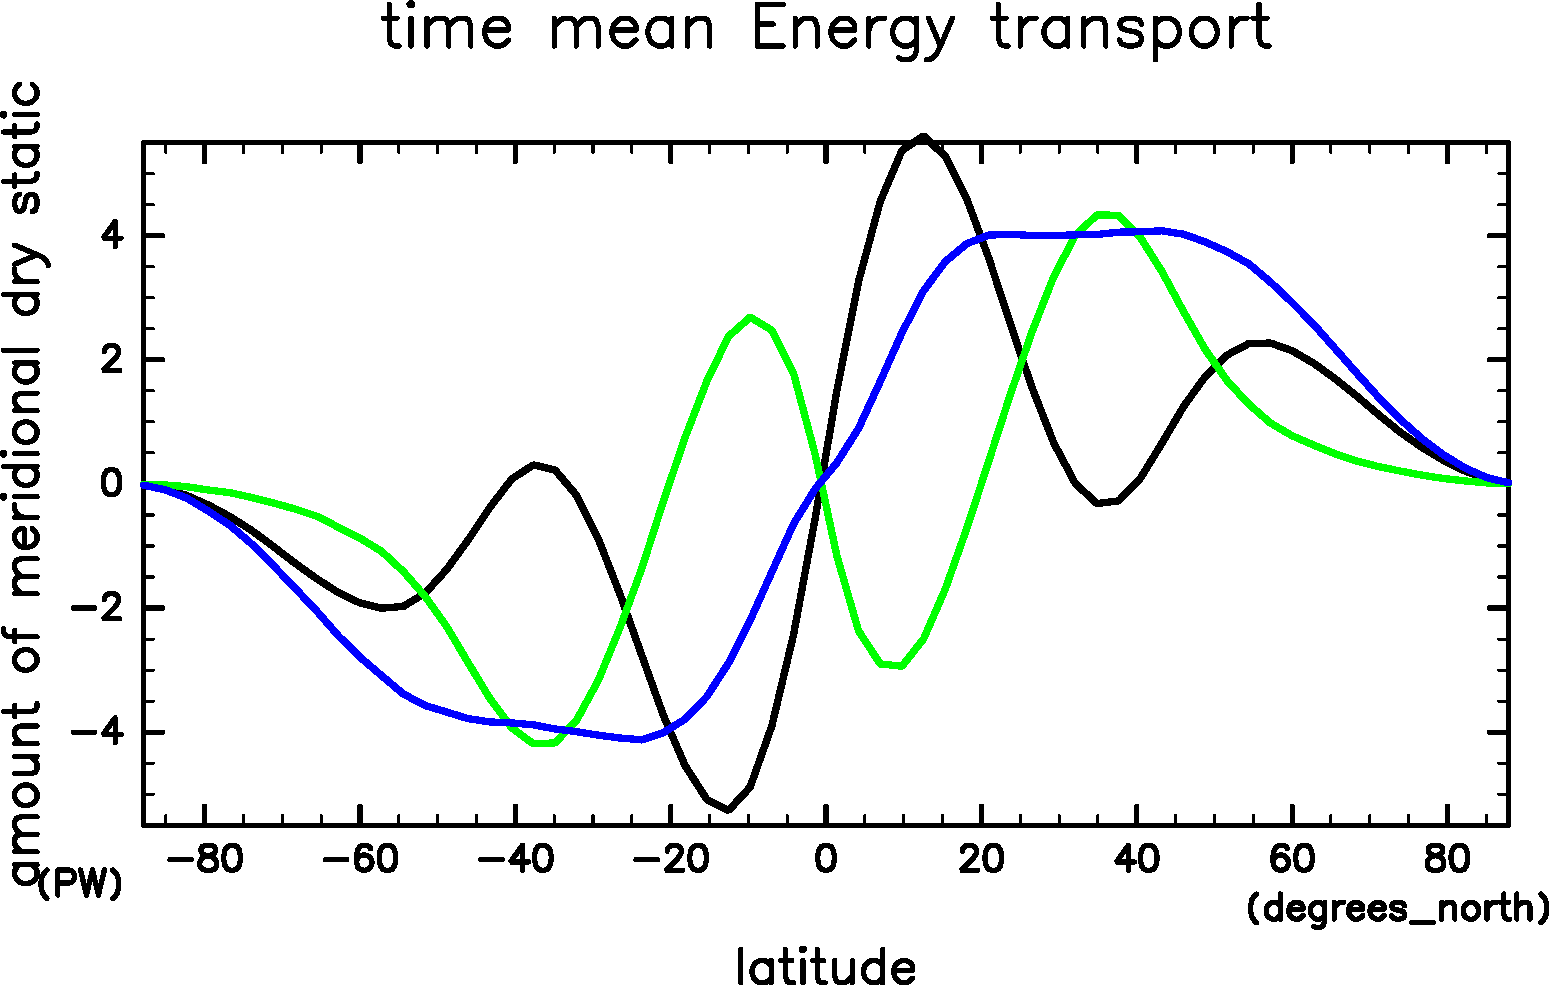
\includegraphics[width=\columnwidth]{S1500/EngyFlx,time=3650:4015-crop-rotate.pdf}
		\caption{\(S=1500\hmu{W/m^2}\)}
	\end{subfigure}
	\begin{subfigure}{.4\textwidth}
		\centering
		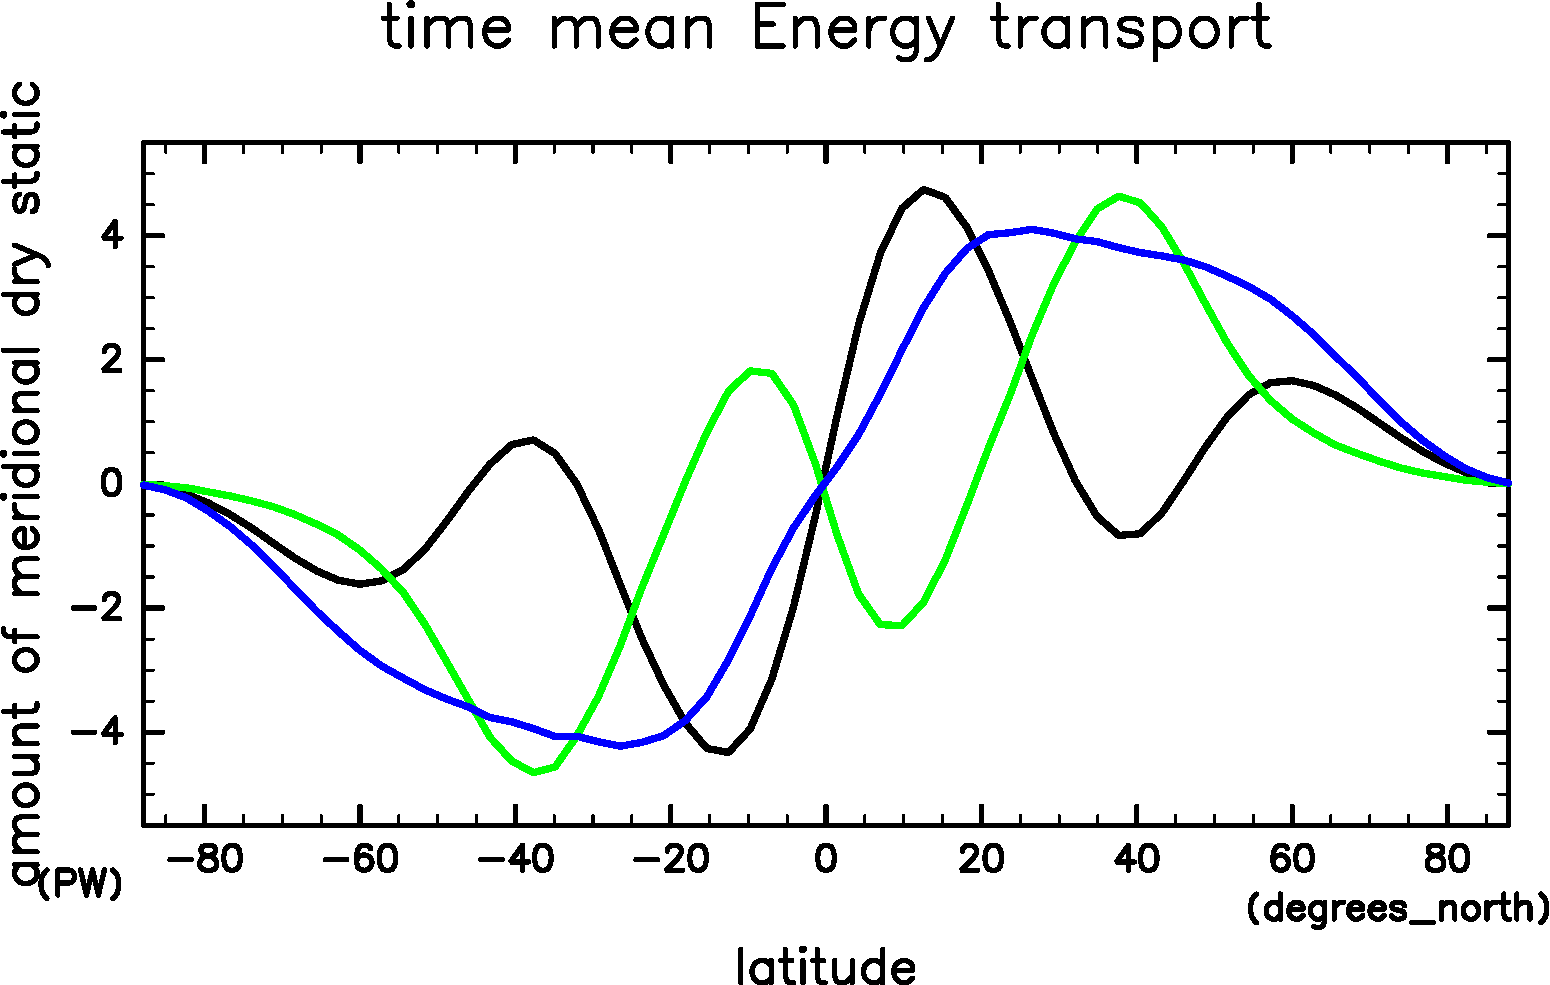
\includegraphics[width=\columnwidth]{S1600/EngyFlx,time=3650:4015-crop-rotate.pdf}
		\caption{\(S=1600\hmu{W/m^2}\)}
	\end{subfigure}
	\begin{subfigure}{.4\textwidth}
		\centering
		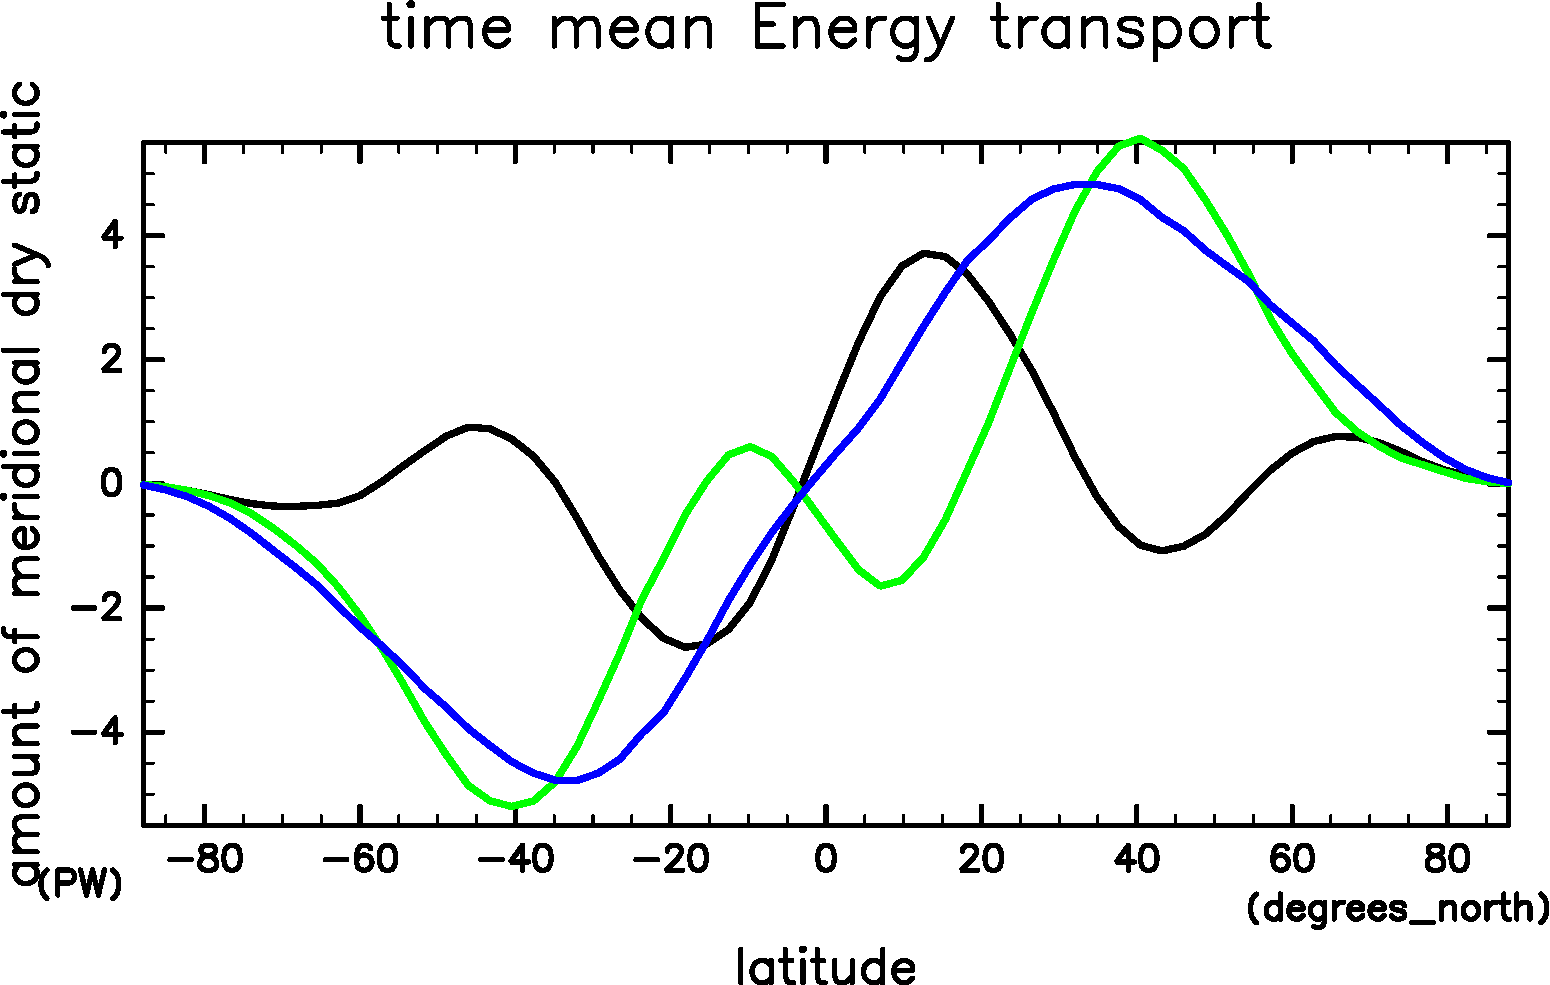
\includegraphics[width=\columnwidth]{S1800/EngyFlx,time=3650:4015-crop-rotate.pdf}
		\caption{\(S=1800\hmu{W/m^2}\)}
	\end{subfigure}
	\begin{subfigure}{.4\textwidth}
		\centering
		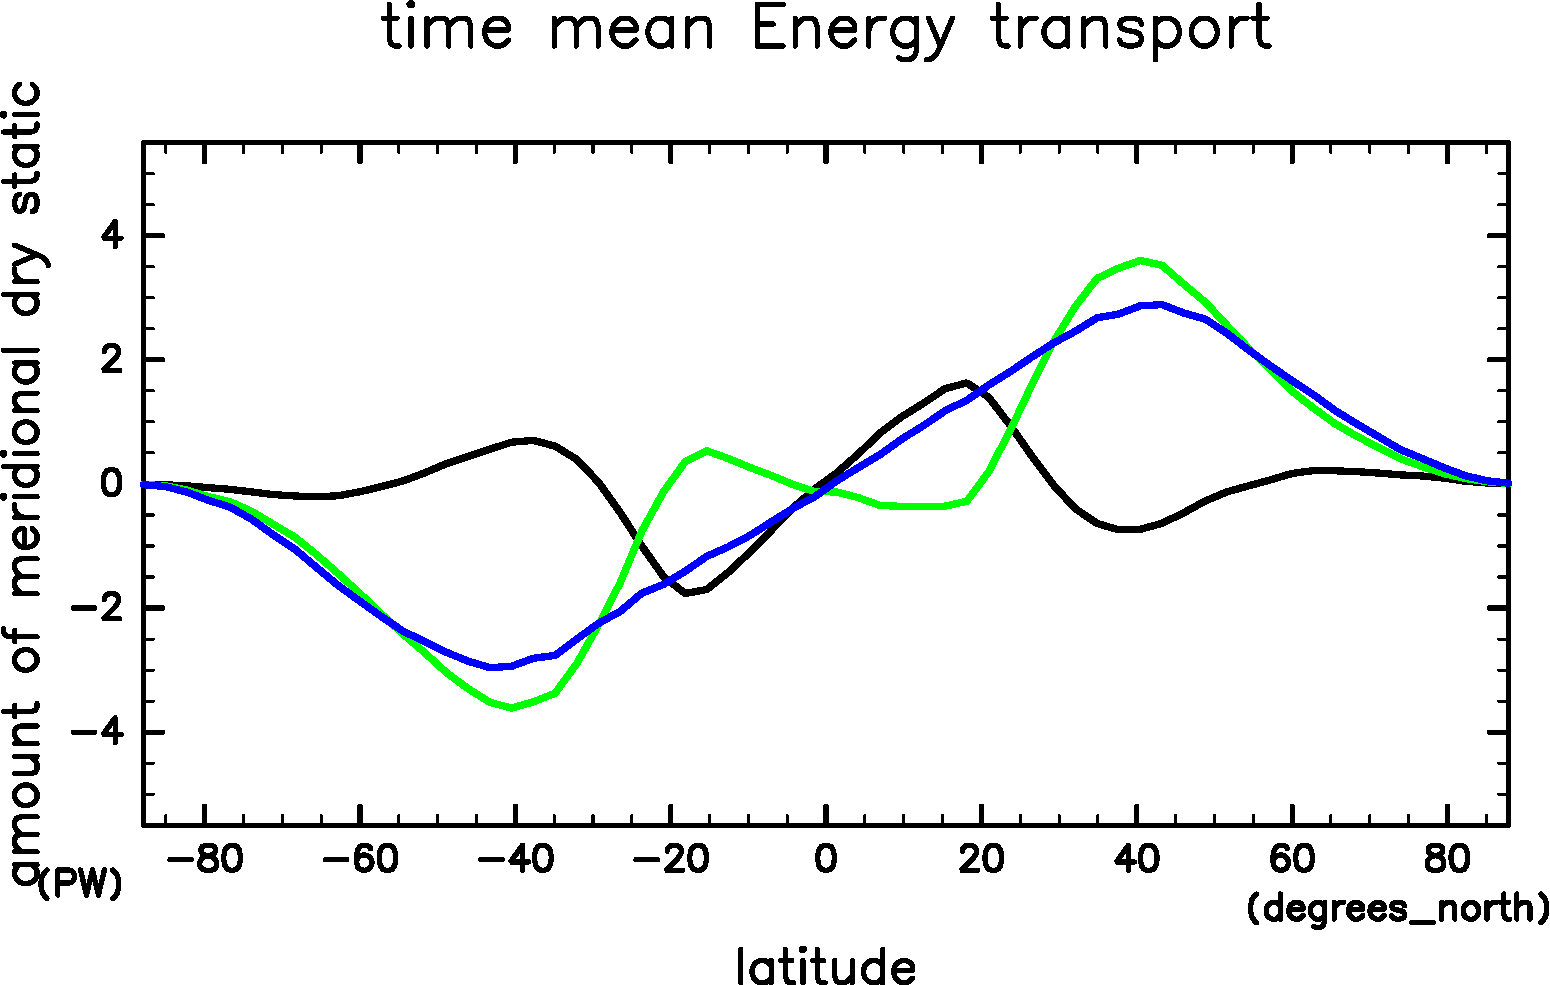
\includegraphics[width=\columnwidth]{S2000/EngyFlx,time=7300:7665-crop-rotate.pdf}
		\caption{\(S=2000\hmu{W/m^2}\)}
	\end{subfigure}
	\caption{
		各実験での南北熱輸送量。緑線が全輸送量、黄線が東西時間平均輸送量、
		桃線が steady eddy transport、青線が transient eddy transport。
	}
\end{figure}

\begin{figure}[t]
	\centering
	\begin{subfigure}{.4\textwidth}
		\centering
		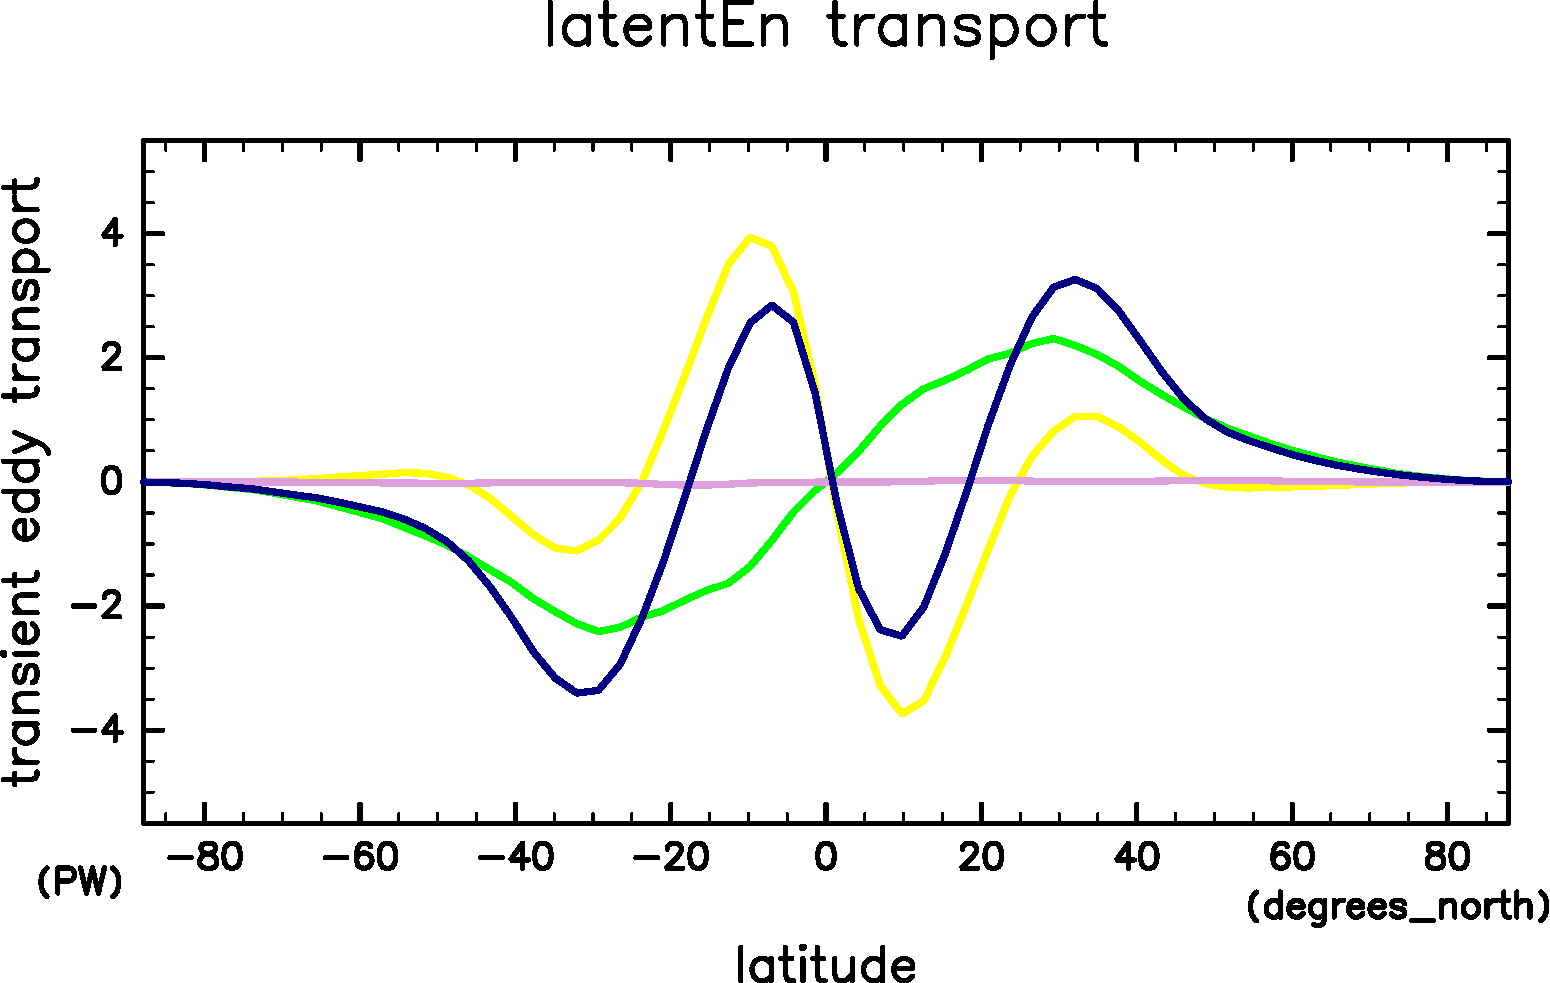
\includegraphics[width=\columnwidth]{S1366/MeriHeatTrans@latentEn,time=14600:14965-crop-rotate.pdf}
		\caption{\(S=1366\hmu{W/m^2}\)}
	\end{subfigure}
	\begin{subfigure}{.4\textwidth}
		\centering
		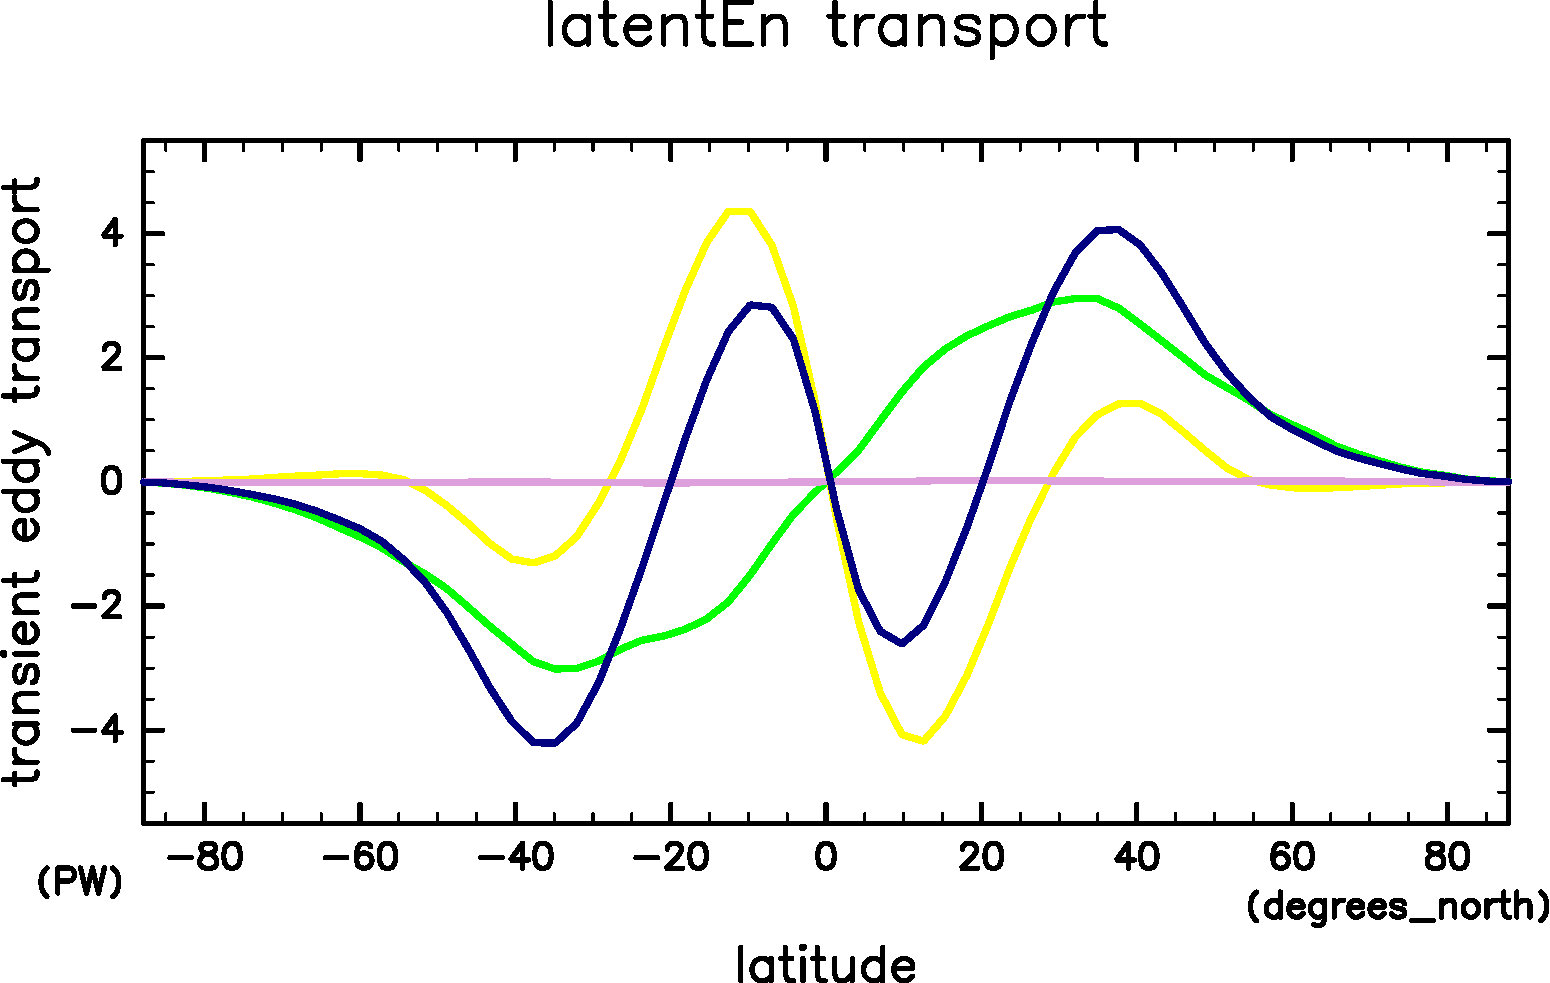
\includegraphics[width=\columnwidth]{S1500/MeriHeatTrans@latentEn,time=3650:4015-crop-rotate.pdf}
		\caption{\(S=1500\hmu{W/m^2}\)}
	\end{subfigure}
	\begin{subfigure}{.4\textwidth}
		\centering
		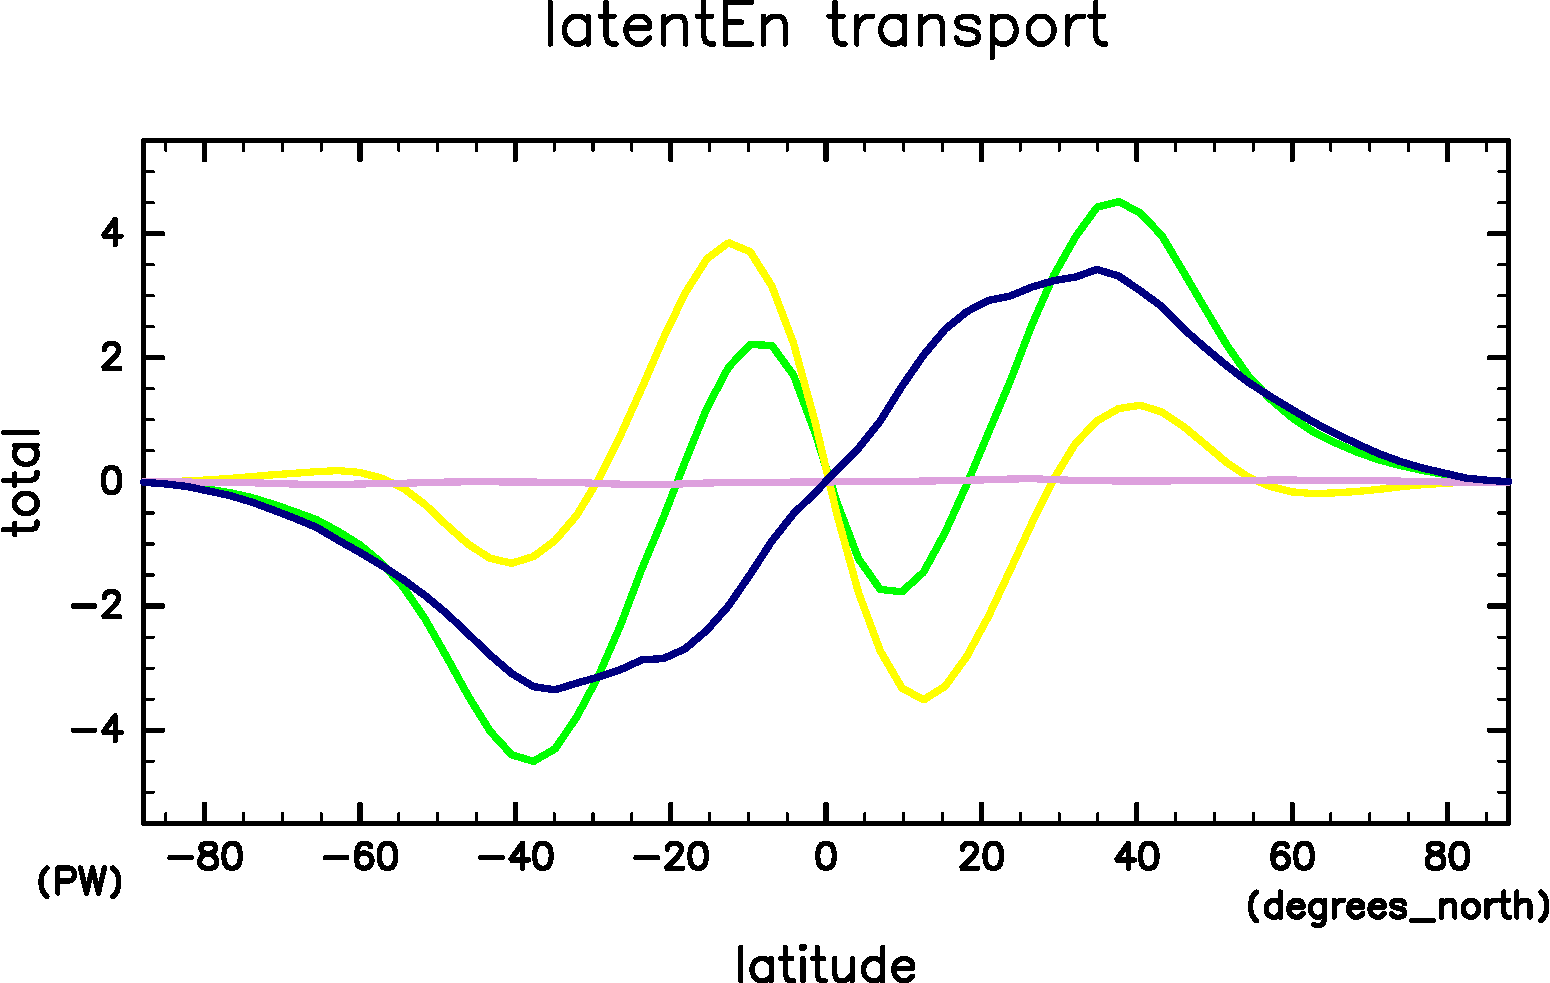
\includegraphics[width=\columnwidth]{S1600/MeriHeatTrans@latentEn,time=3650:4015-crop-rotate.pdf}
		\caption{\(S=1600\hmu{W/m^2}\)}
	\end{subfigure}
	\begin{subfigure}{.4\textwidth}
		\centering
		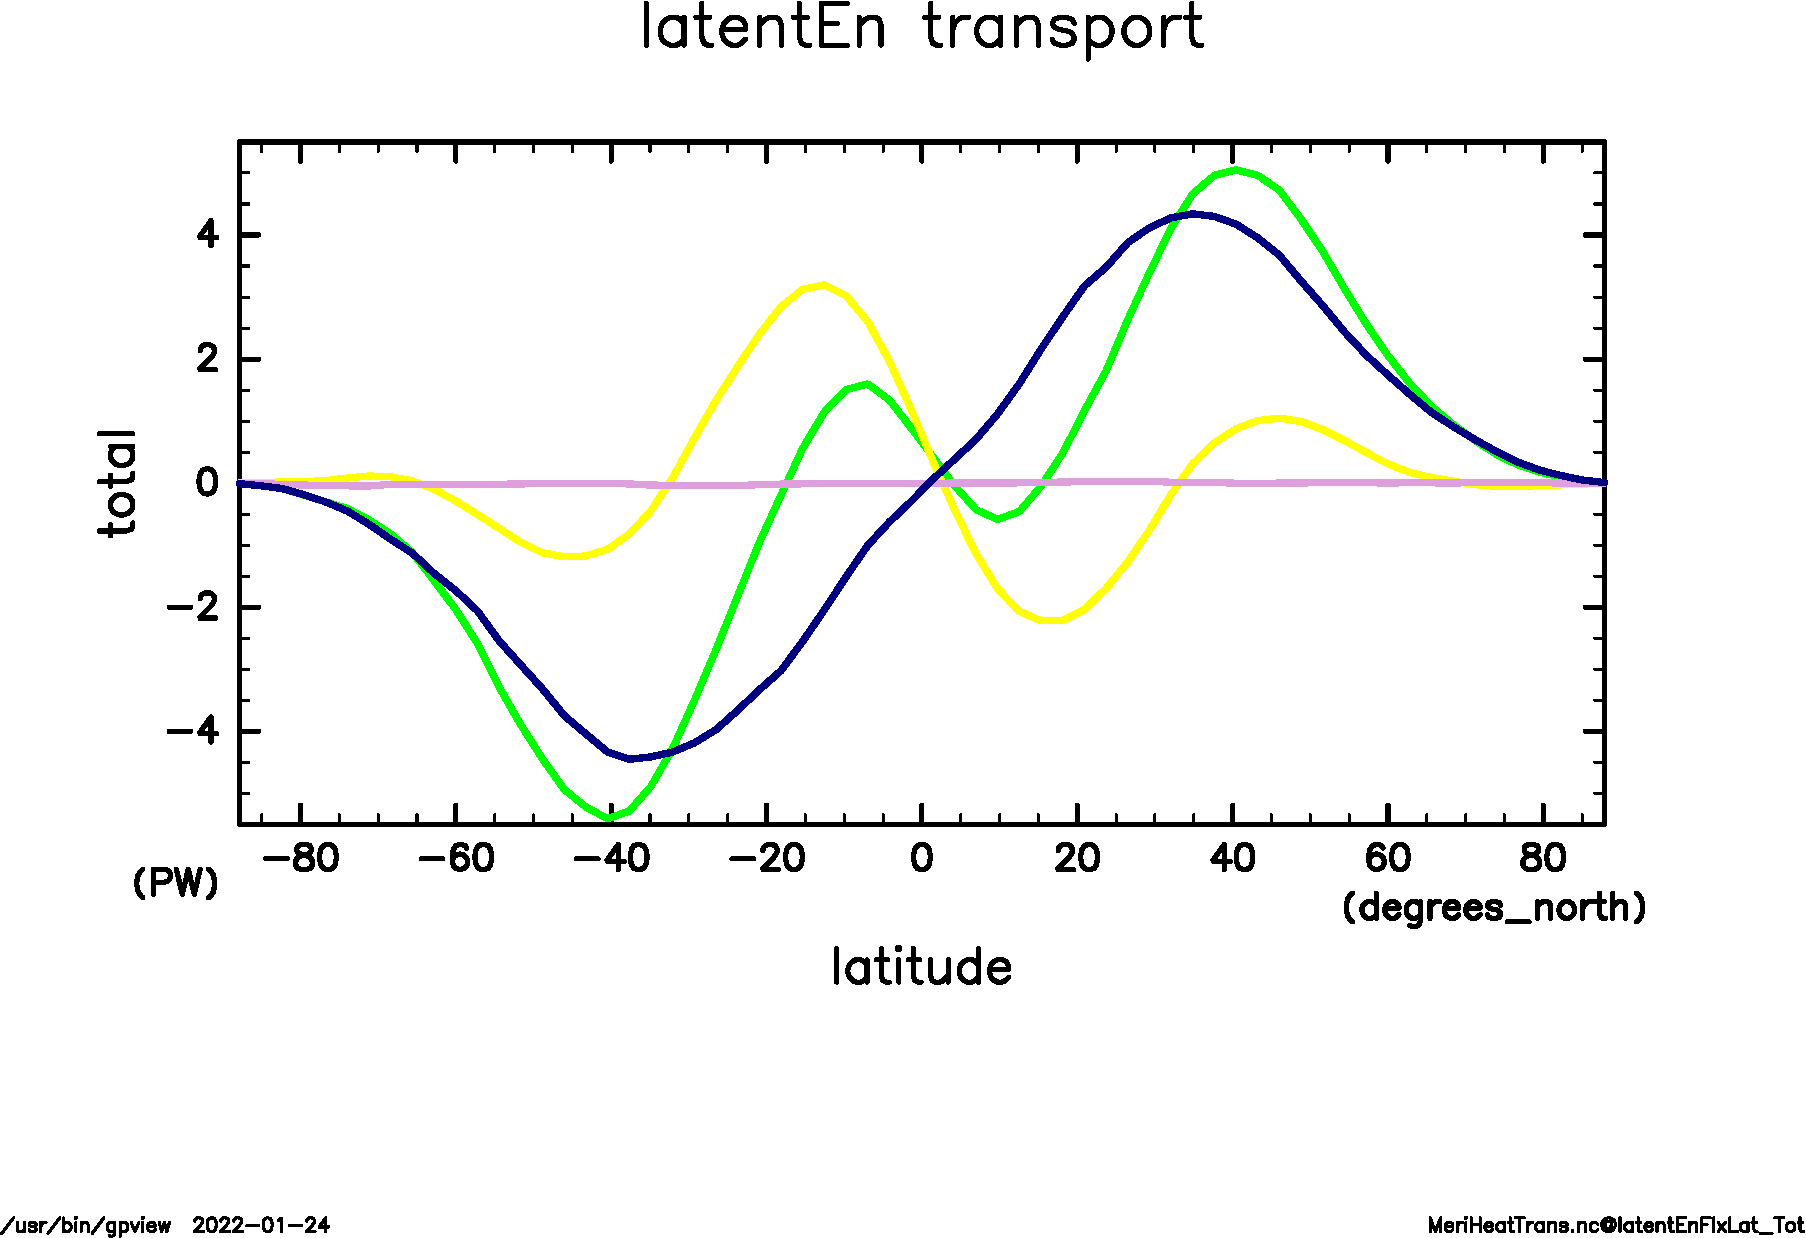
\includegraphics[width=\columnwidth]{S1800/MeriHeatTrans@latentEn,time=3650:4015-crop-rotate.pdf}
		\caption{\(S=1800\hmu{W/m^2}\)}
	\end{subfigure}
	\begin{subfigure}{.4\textwidth}
		\centering
		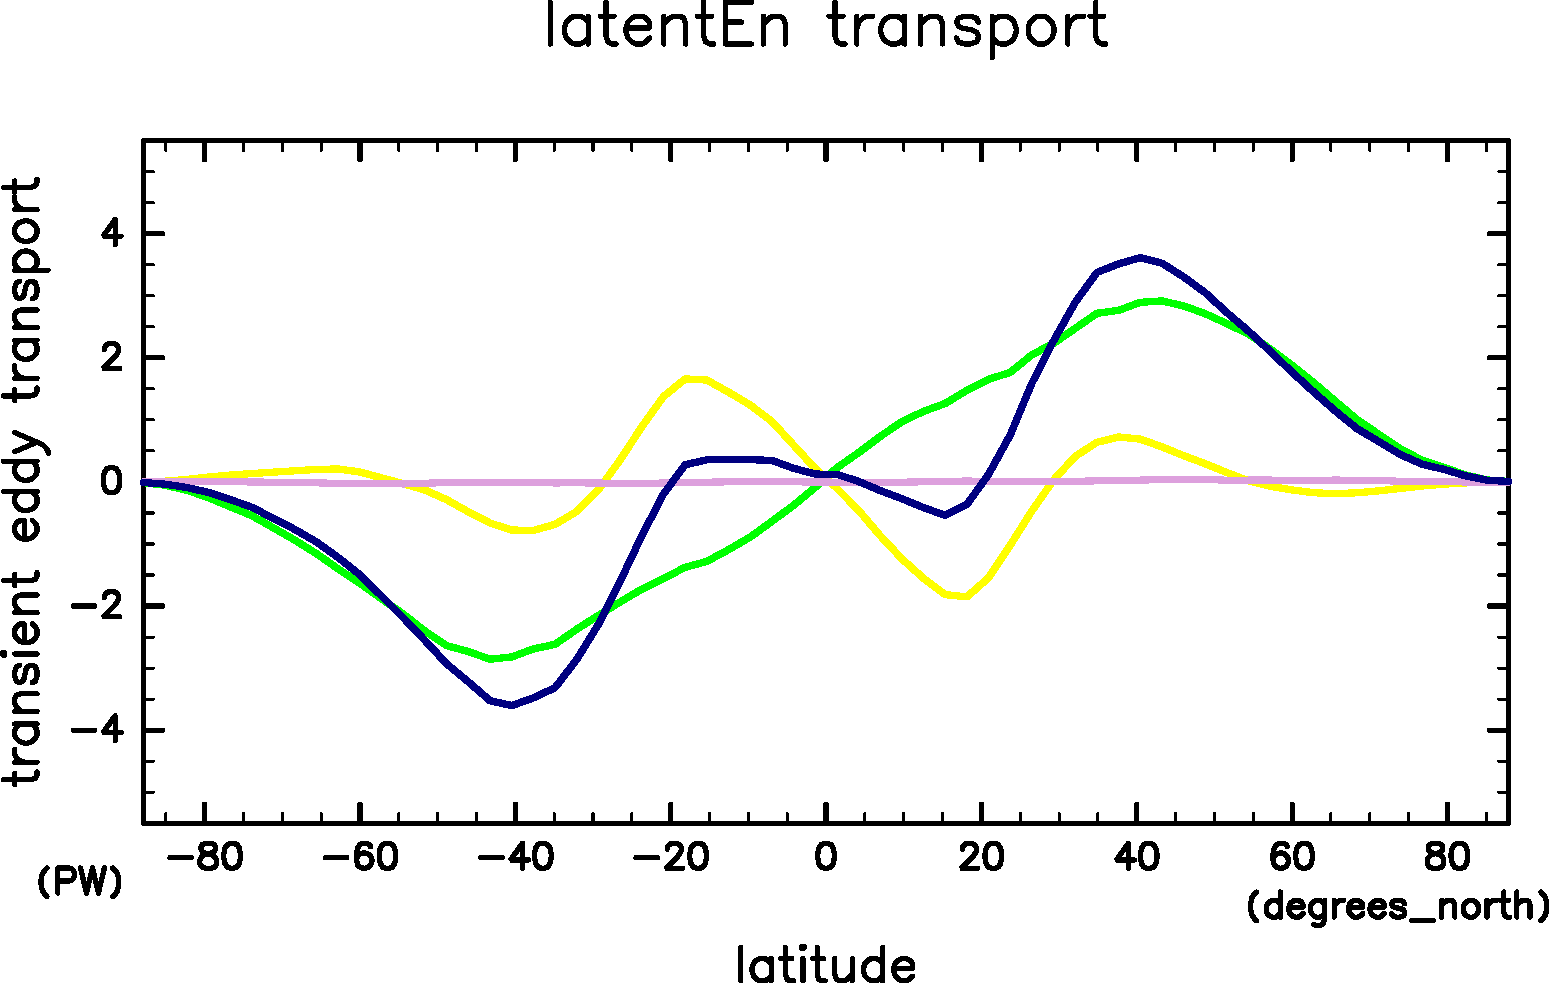
\includegraphics[width=\columnwidth]{S2000/MeriHeatTrans@latentEn,time=7300:7665-crop-rotate.pdf}
		\caption{\(S=2000\hmu{W/m^2}\)}
	\end{subfigure}
	\caption{
		各実験での潜熱輸送。緑線が全輸送量、黄線が東西時間平均輸送量、
		桃線が steady eddy transport、青線が transient eddy transport。
	}
\end{figure}

\begin{figure}[t]
	\centering
	\begin{subfigure}{.4\textwidth}
		\centering
		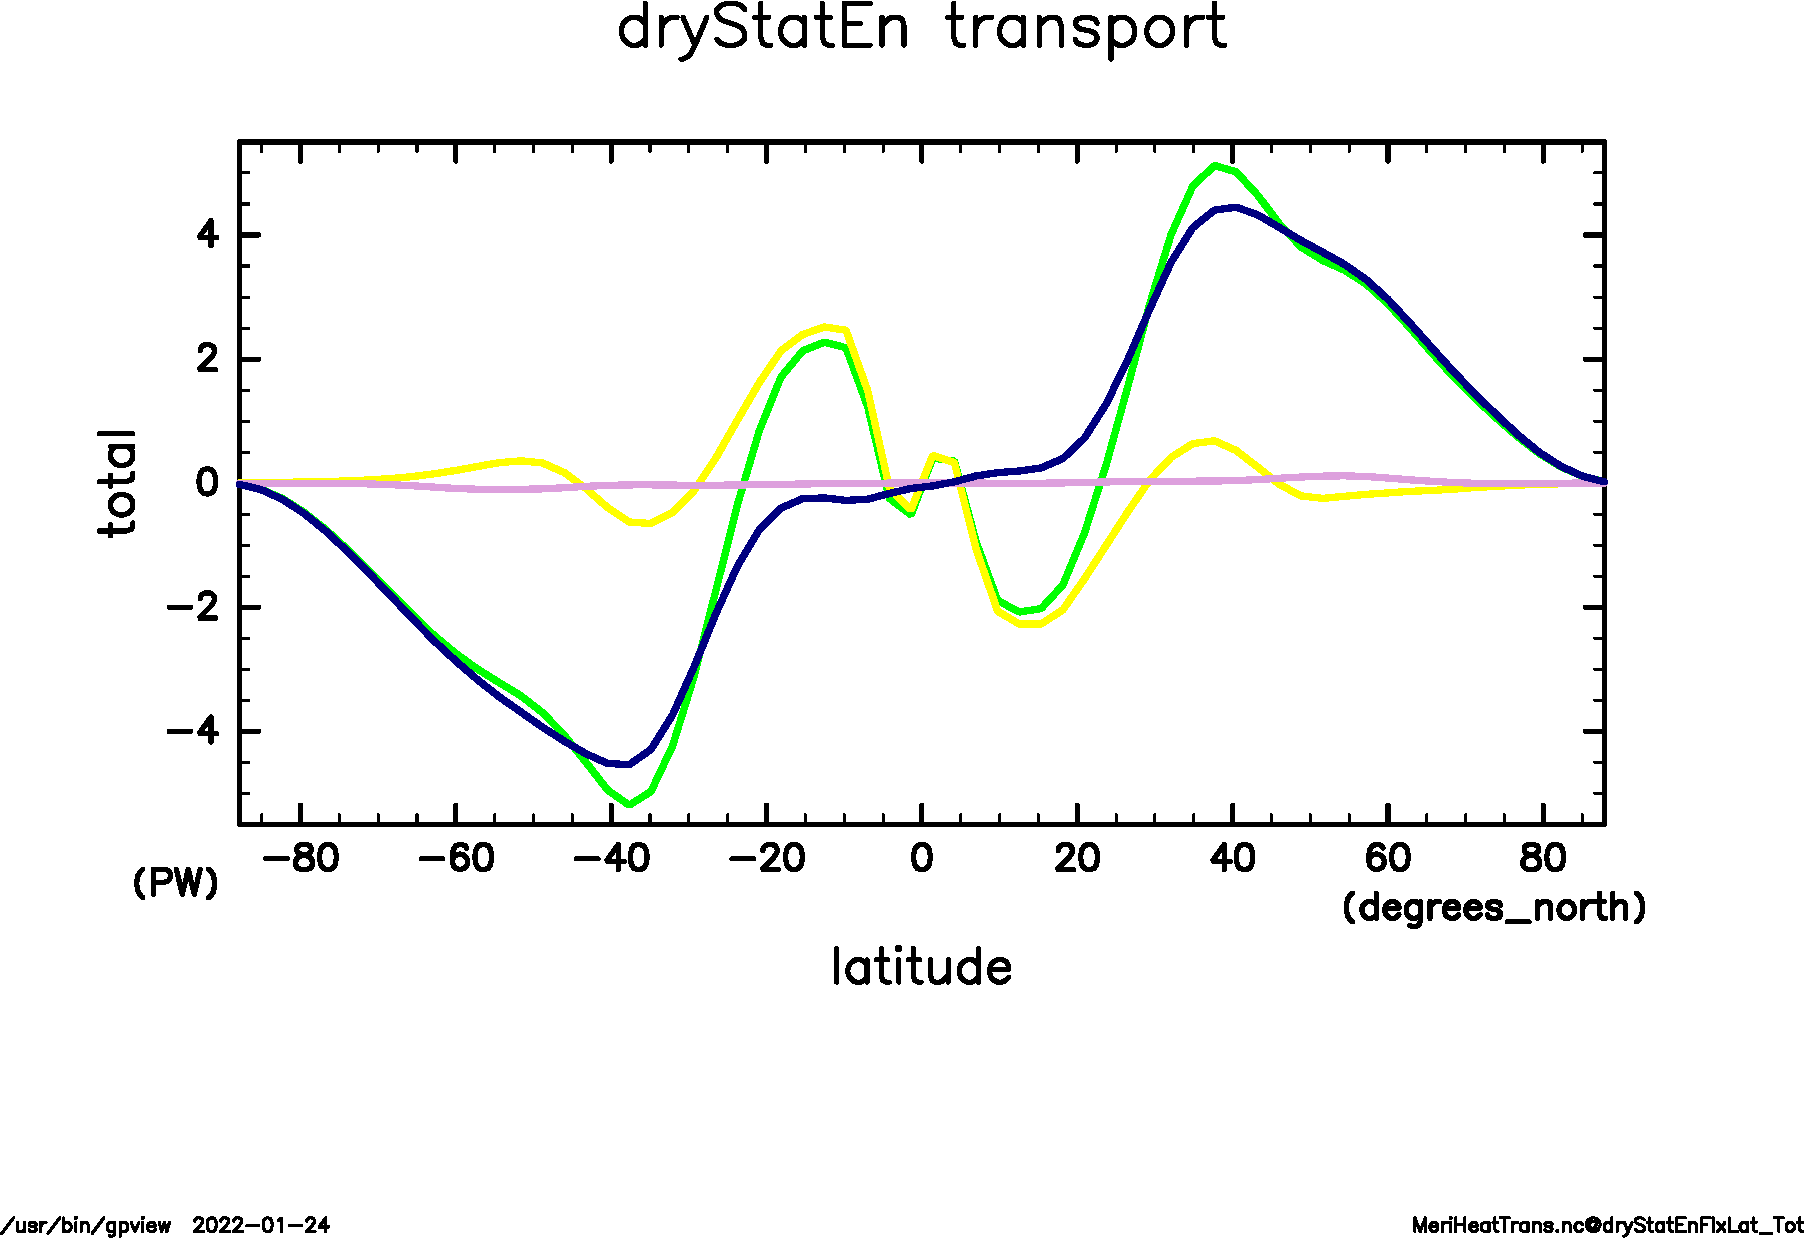
\includegraphics[width=\columnwidth]{S1366/MeriHeatTrans@dryStatEn,time=14600:14965-crop-rotate.pdf}
		\caption{\(S=1366\hmu{W/m^2}\)}
	\end{subfigure}
	\begin{subfigure}{.4\textwidth}
		\centering
		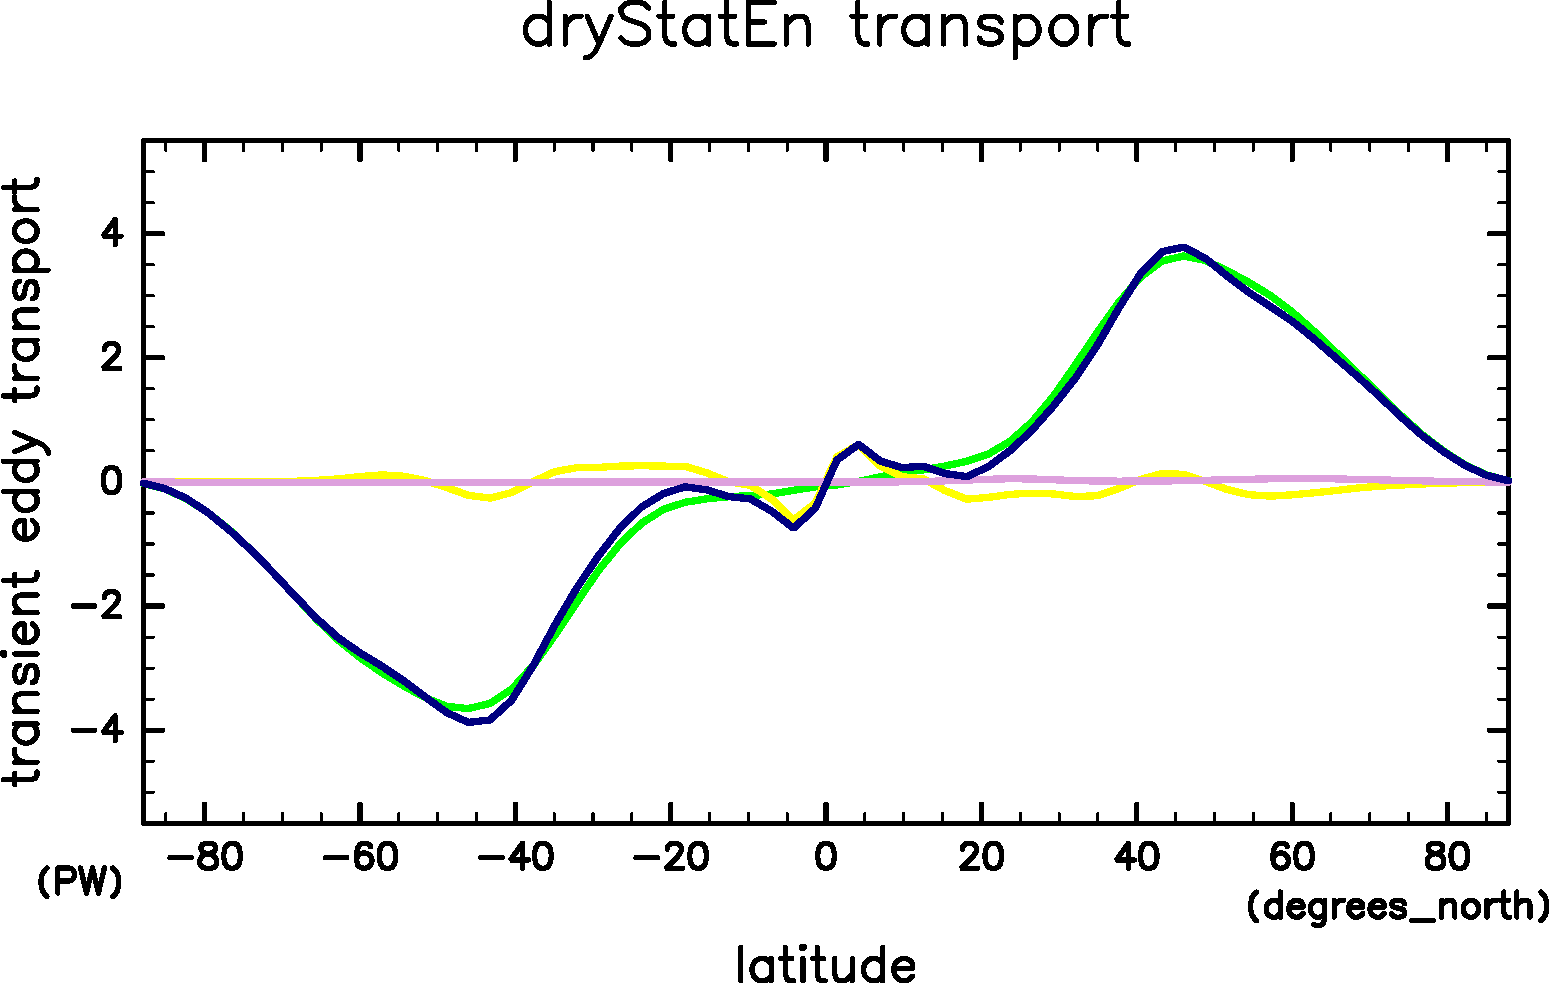
\includegraphics[width=\columnwidth]{S1500/MeriHeatTrans@dryStatEn,time=3650:4015-crop-rotate.pdf}
		\caption{\(S=1500\hmu{W/m^2}\)}
	\end{subfigure}
	\begin{subfigure}{.4\textwidth}
		\centering
		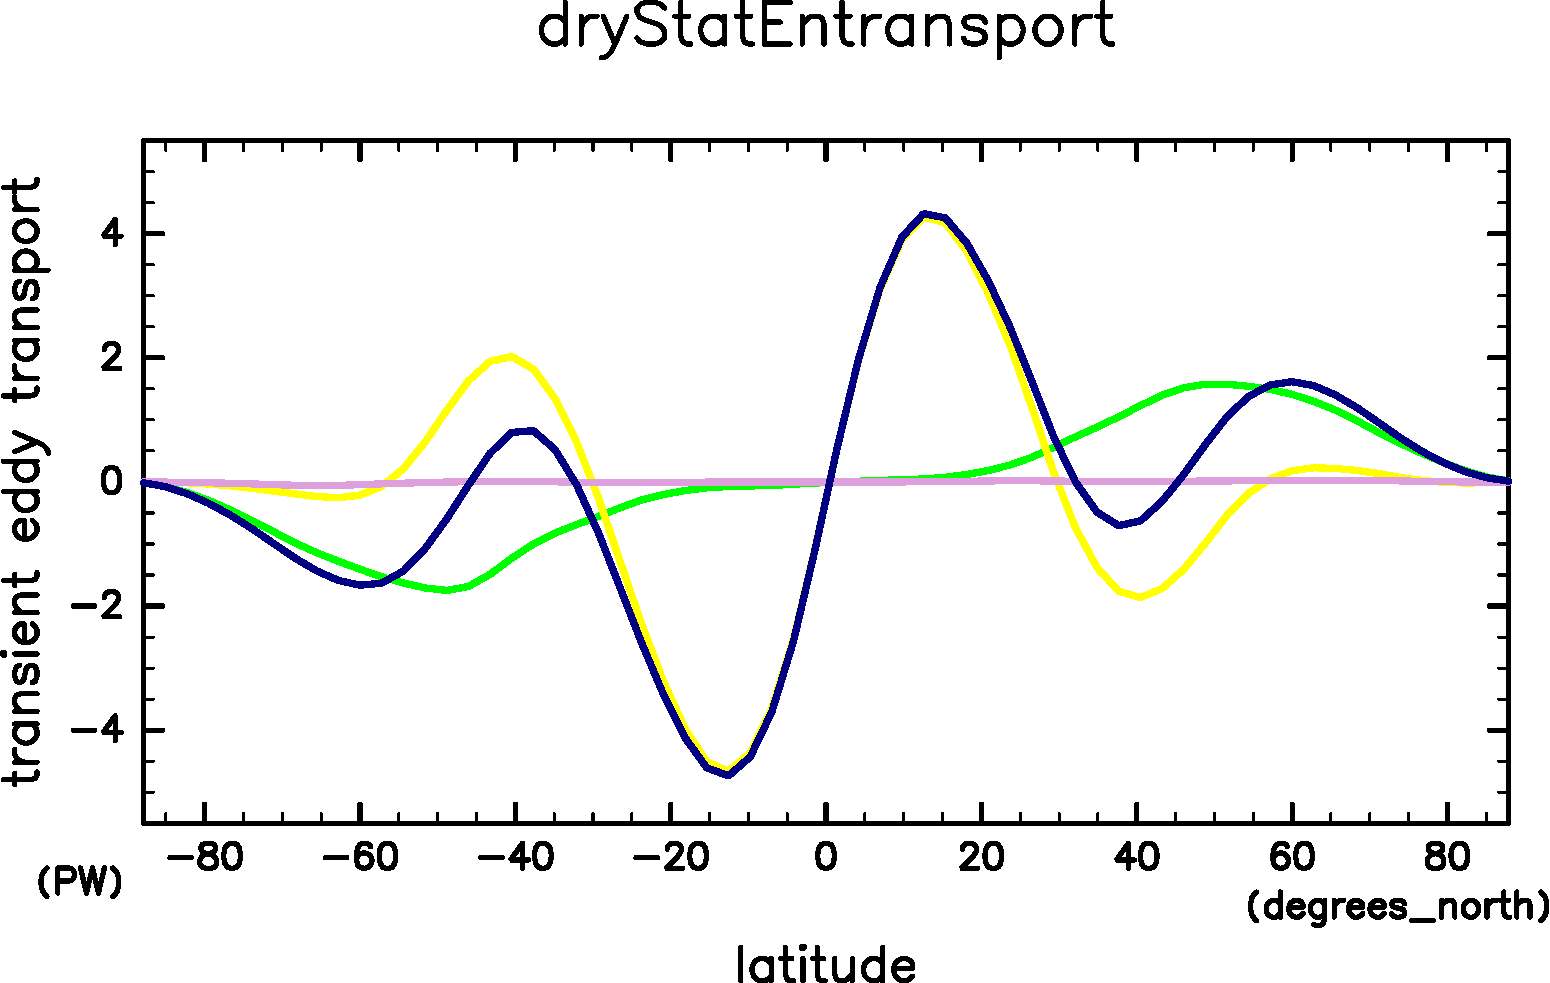
\includegraphics[width=\columnwidth]{S1600/MeriHeatTrans@dryStatEn,time=3650:4015-crop-rotate.pdf}
		\caption{\(S=1600\hmu{W/m^2}\)}
	\end{subfigure}
	\begin{subfigure}{.4\textwidth}
		\centering
		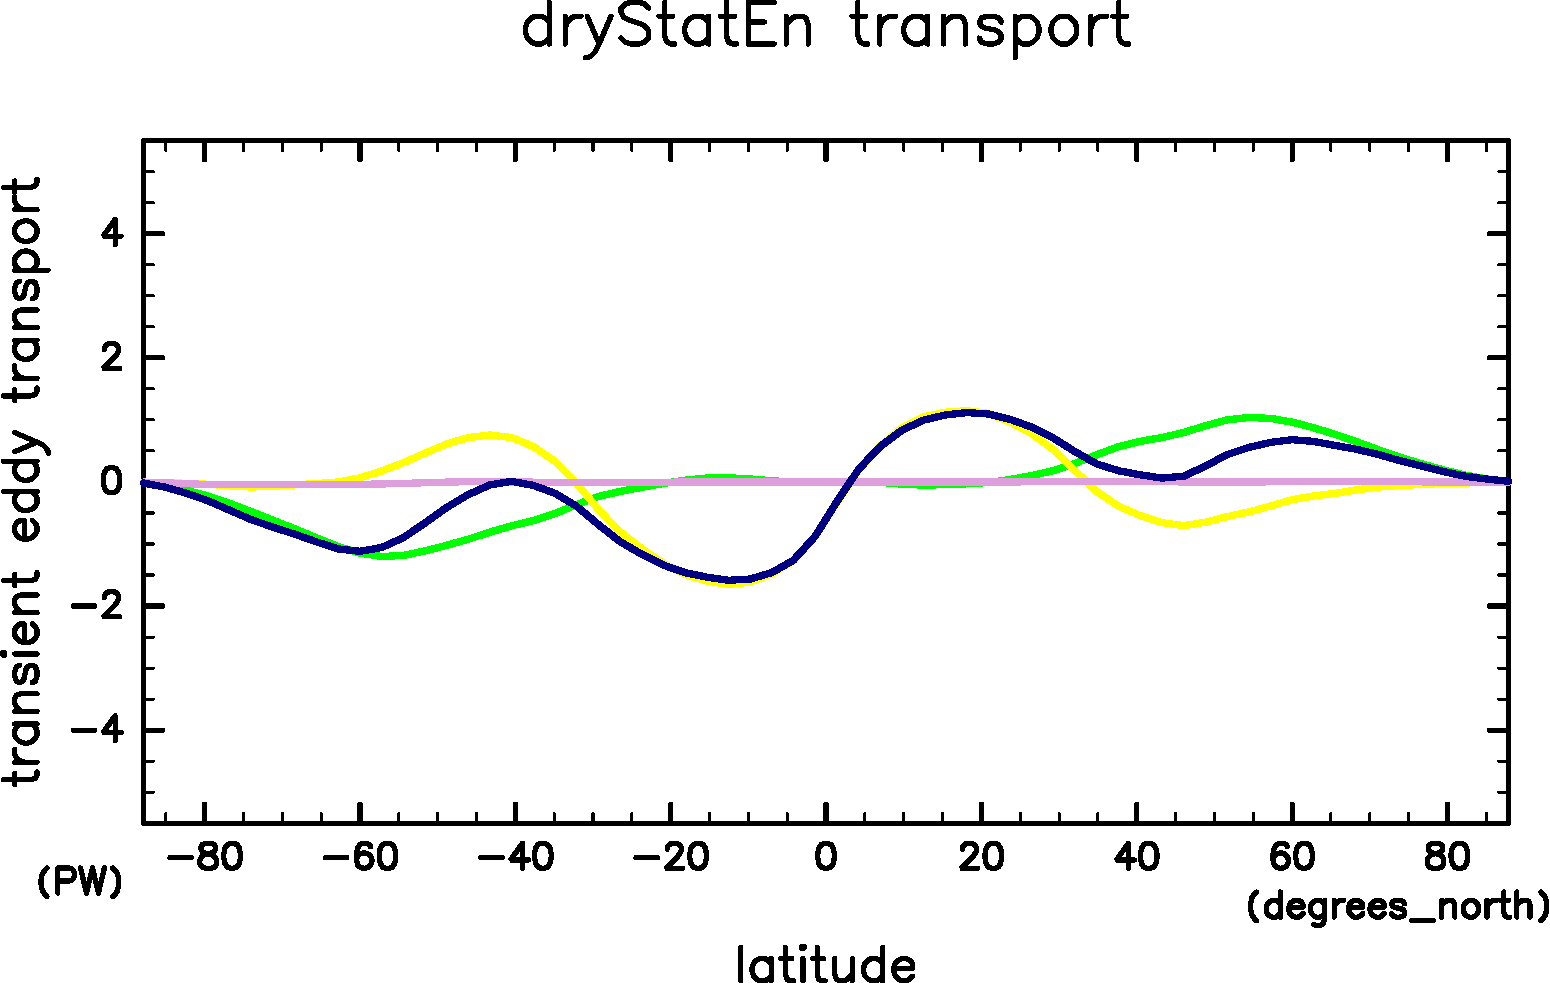
\includegraphics[width=\columnwidth]{S1800/MeriHeatTrans@dryStatEn,time=3650:4015-crop-rotate.pdf}
		\caption{\(S=1800\hmu{W/m^2}\)}
	\end{subfigure}
	\begin{subfigure}{.4\textwidth}
		\centering
		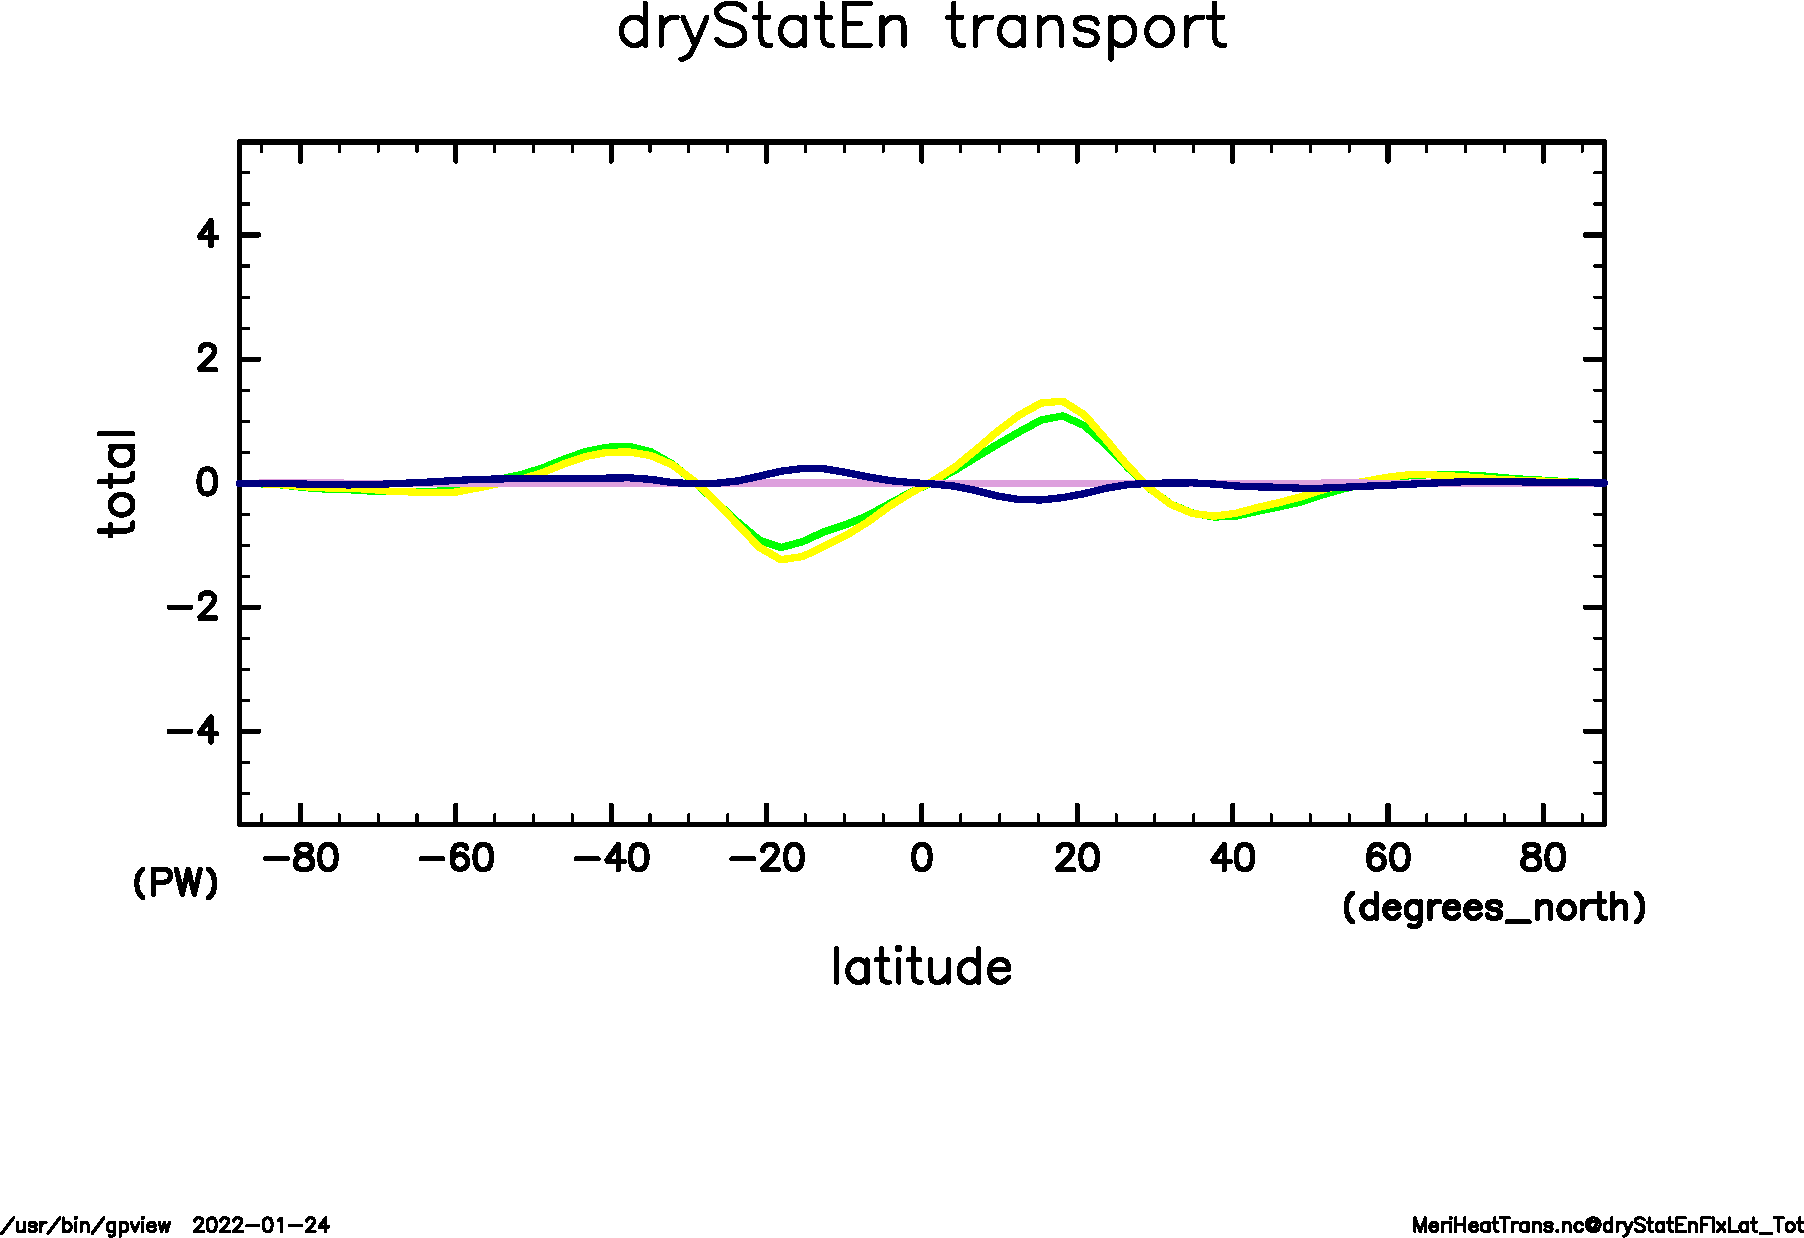
\includegraphics[width=\columnwidth]{S2000/MeriHeatTrans@dryStatEn,time=7300:7665-crop-rotate.pdf}
		\caption{\(S=2000\hmu{W/m^2}\)}
	\end{subfigure}
	\caption{
		各実験での乾燥静的エネルギー輸送。緑線が全輸送量、黄線が東西時間平均輸送量、
		桃線が steady eddy transport、青線が transient eddy transport。
	}
\end{figure}

\begin{figure}[t]
	\centering
	\begin{subfigure}{.4\textwidth}
		\centering
		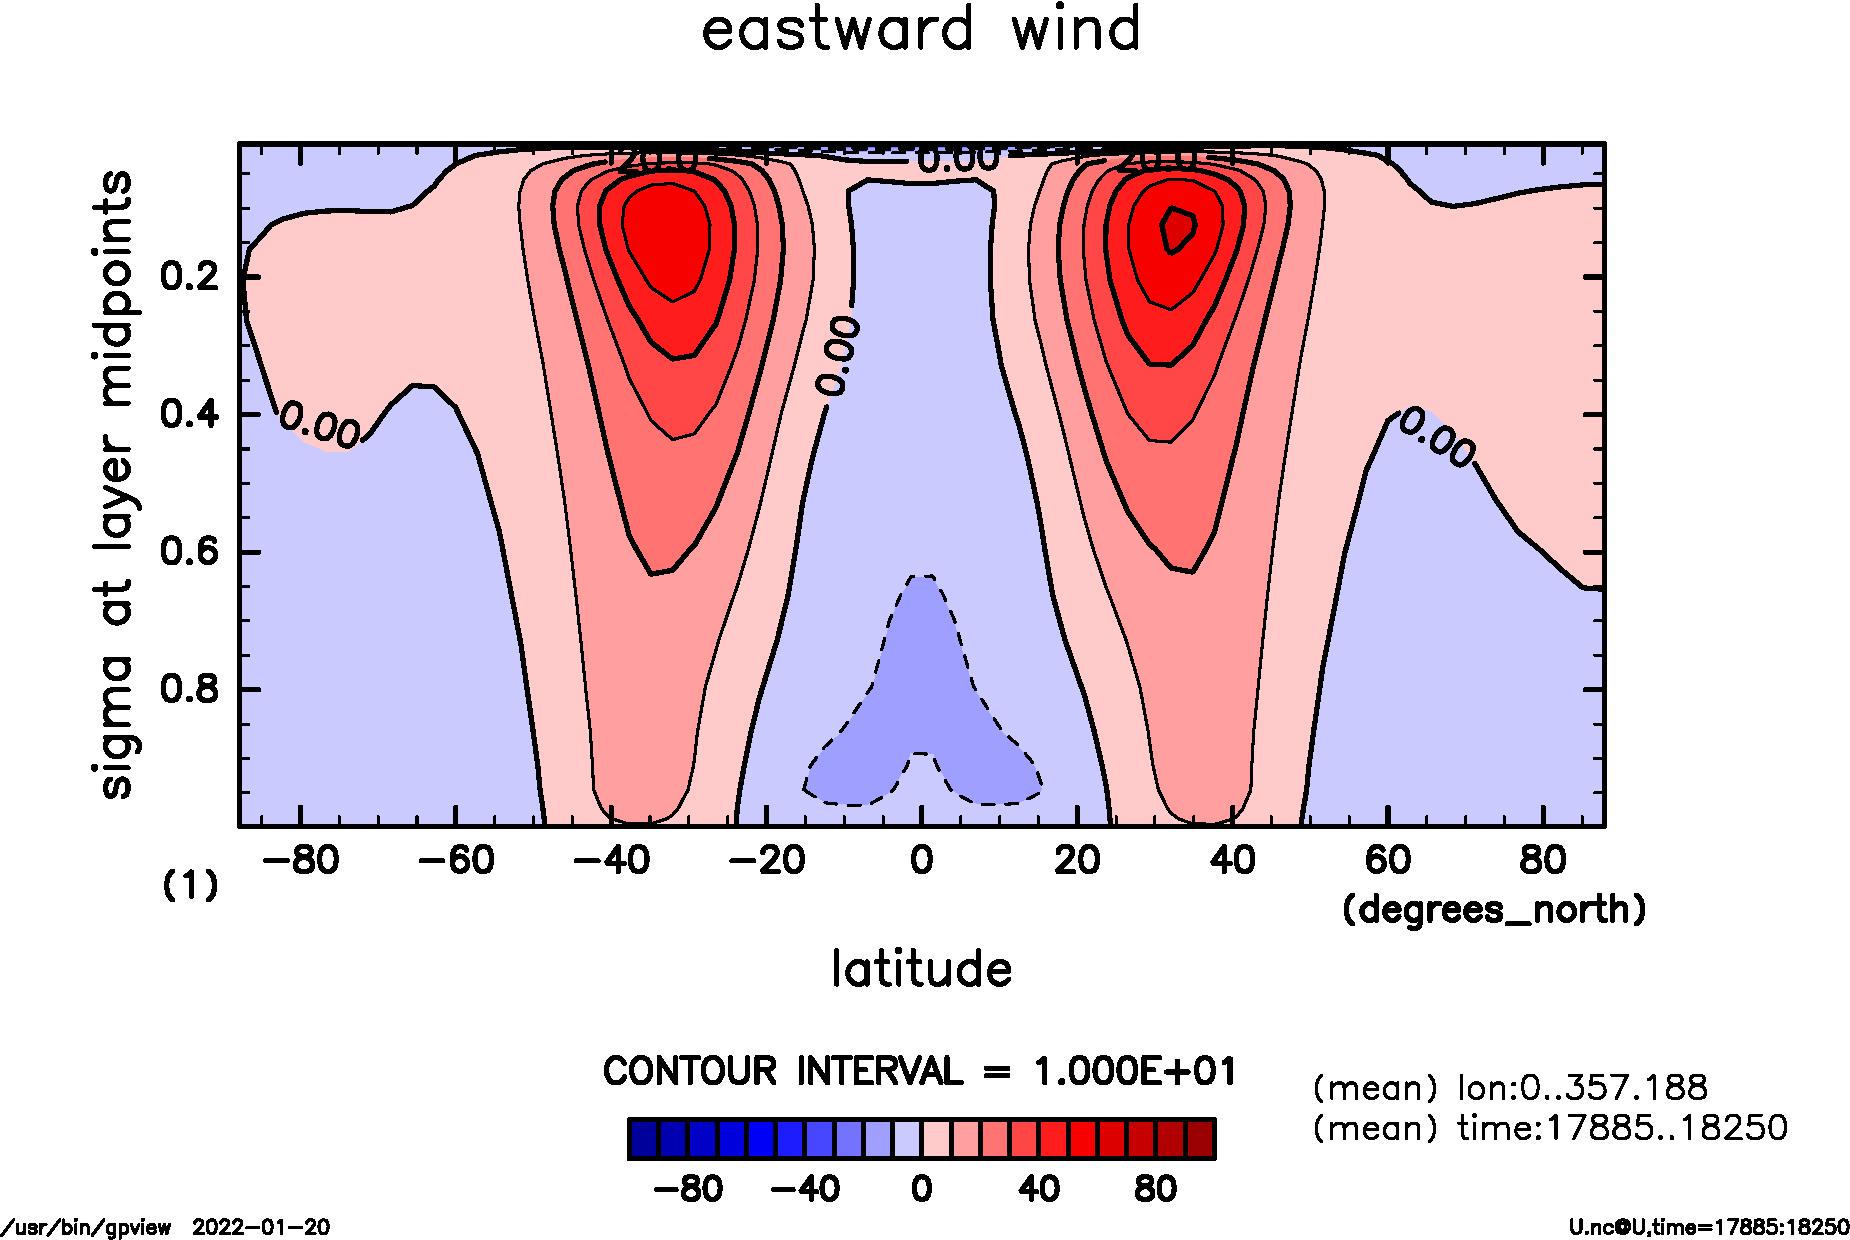
\includegraphics[width=\columnwidth]{S1366/U,time=17885:18250-crop-rotate.pdf}
		\caption{東西風}
	\end{subfigure}
	\begin{subfigure}{.4\textwidth}
		\centering
		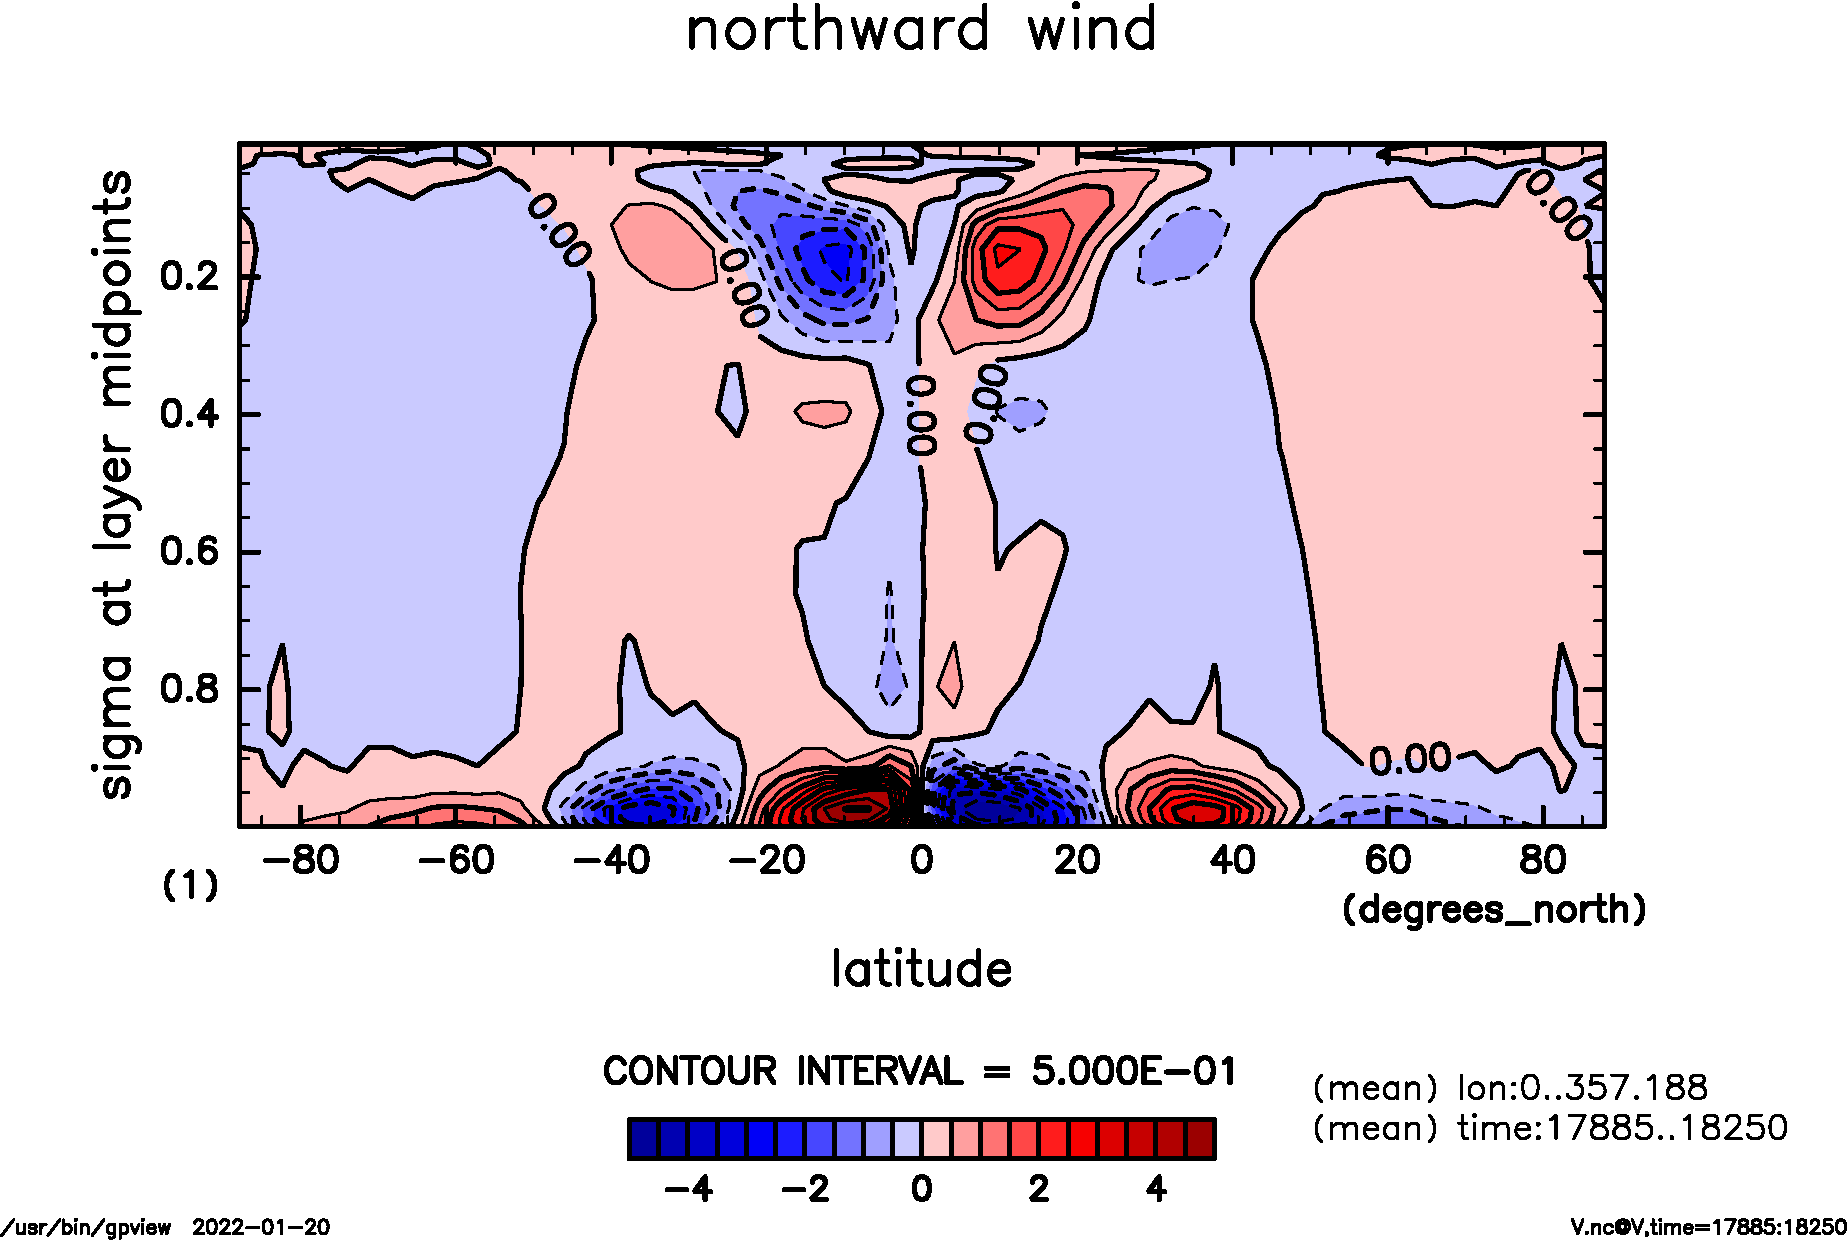
\includegraphics[width=\columnwidth]{S1366/V,time=17885:18250-crop-rotate.pdf}
		\caption{南北風}
	\end{subfigure}
	\begin{subfigure}{.4\textwidth}
		\centering
		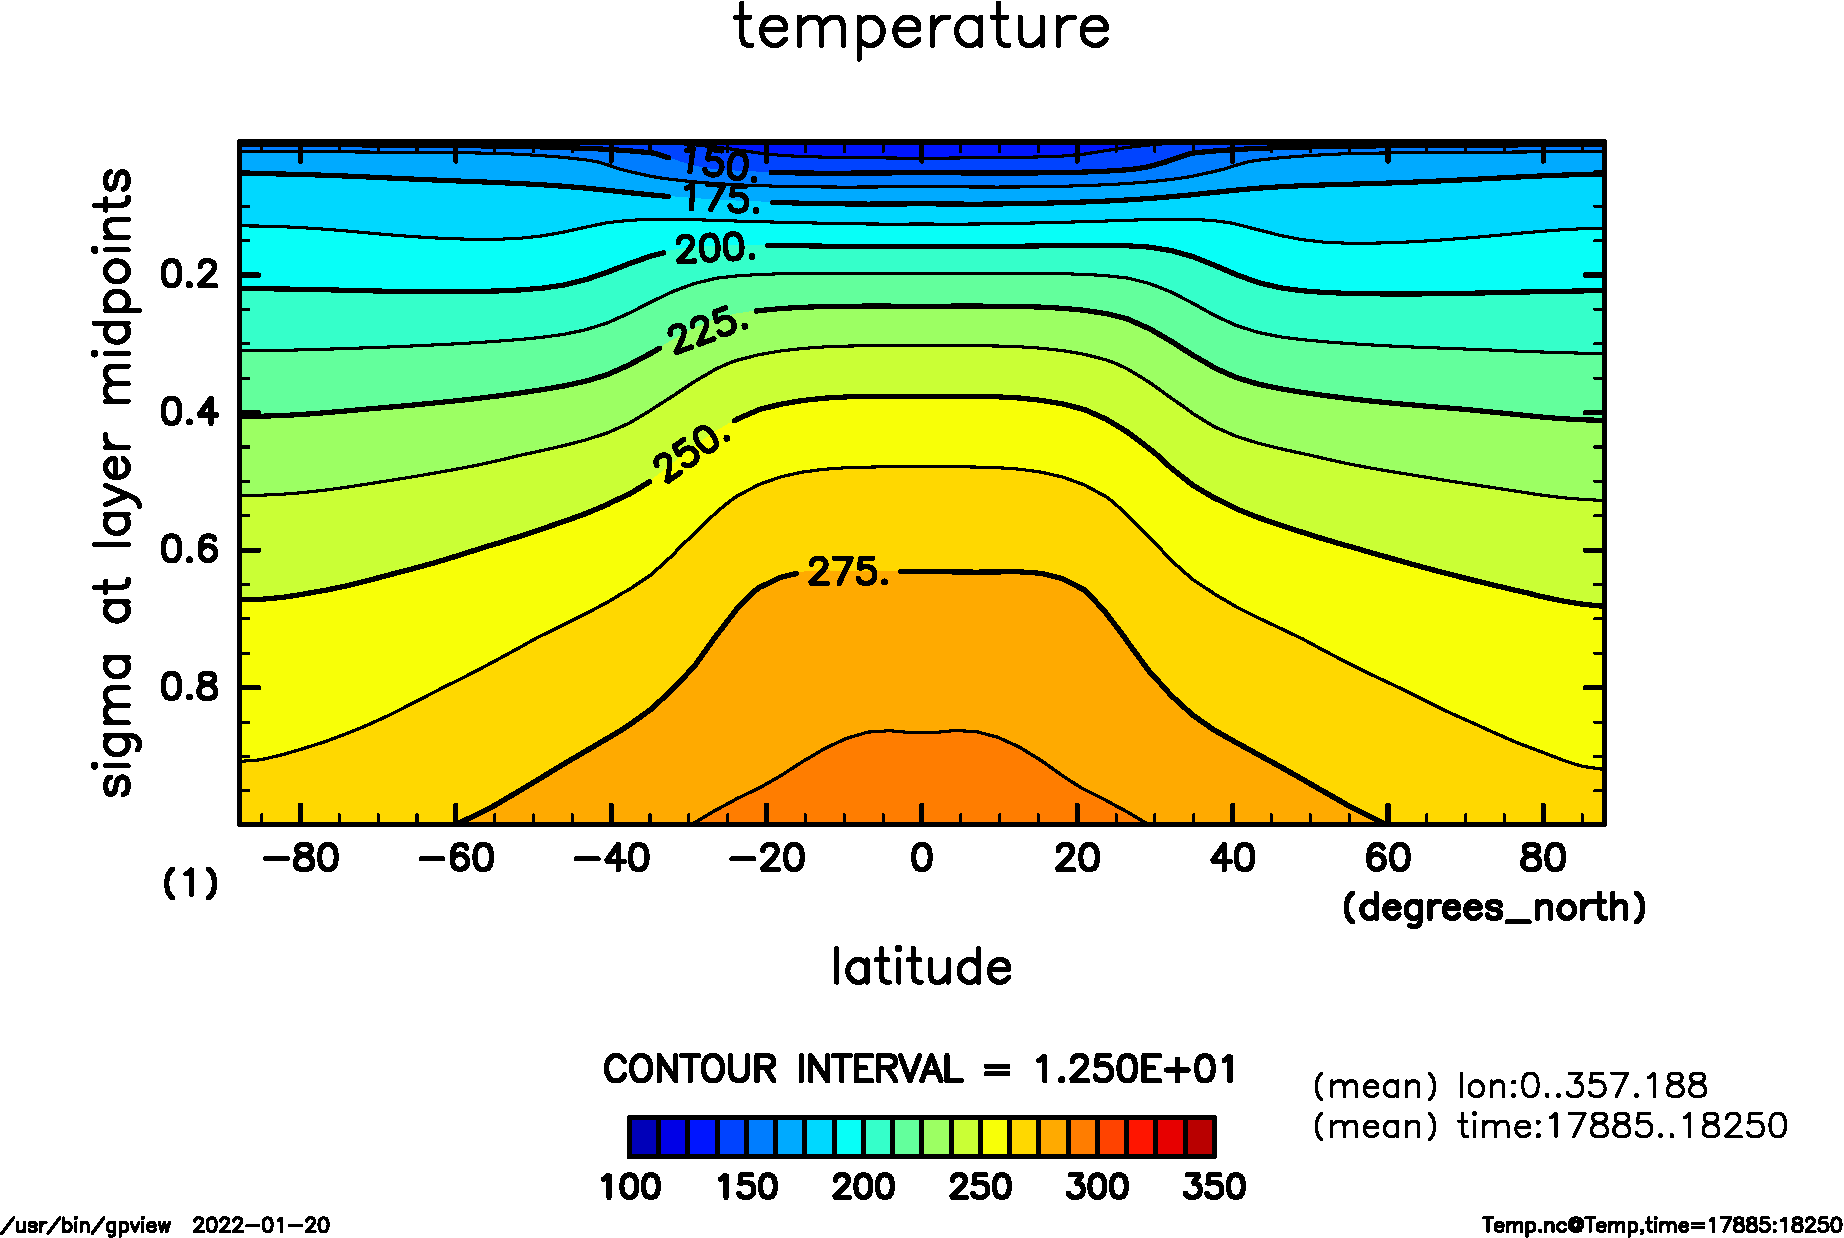
\includegraphics[width=\columnwidth]{S1366/Temp,time=17885:18250-crop-rotate.pdf}
		\caption{気温分布}
	\end{subfigure}
	\begin{subfigure}{.4\textwidth}
		\centering
		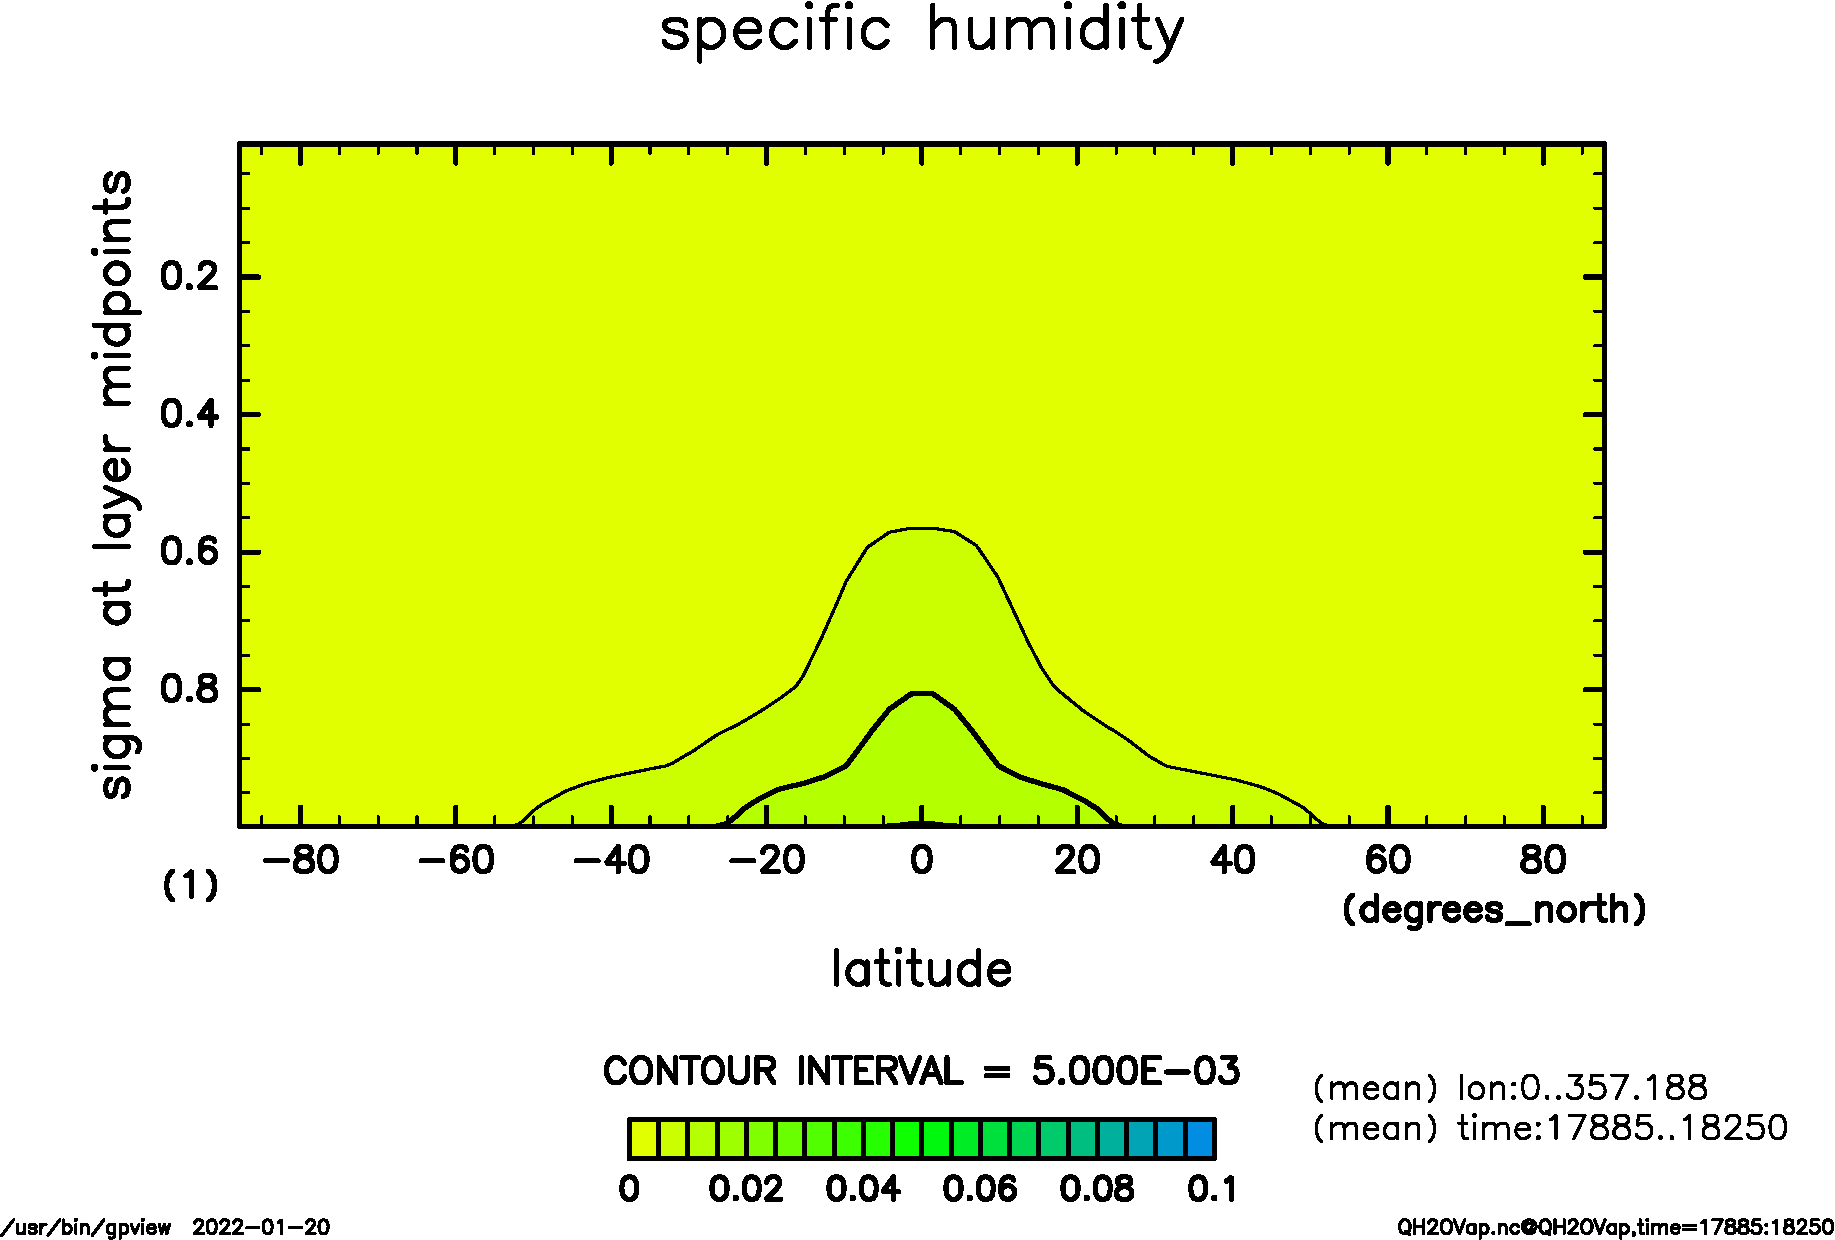
\includegraphics[width=\columnwidth]{S1366/QH2OVap,time=17885:18250-crop-rotate.pdf}
		\caption{比湿}
	\end{subfigure}
	\begin{subfigure}{.4\textwidth}
		\centering
		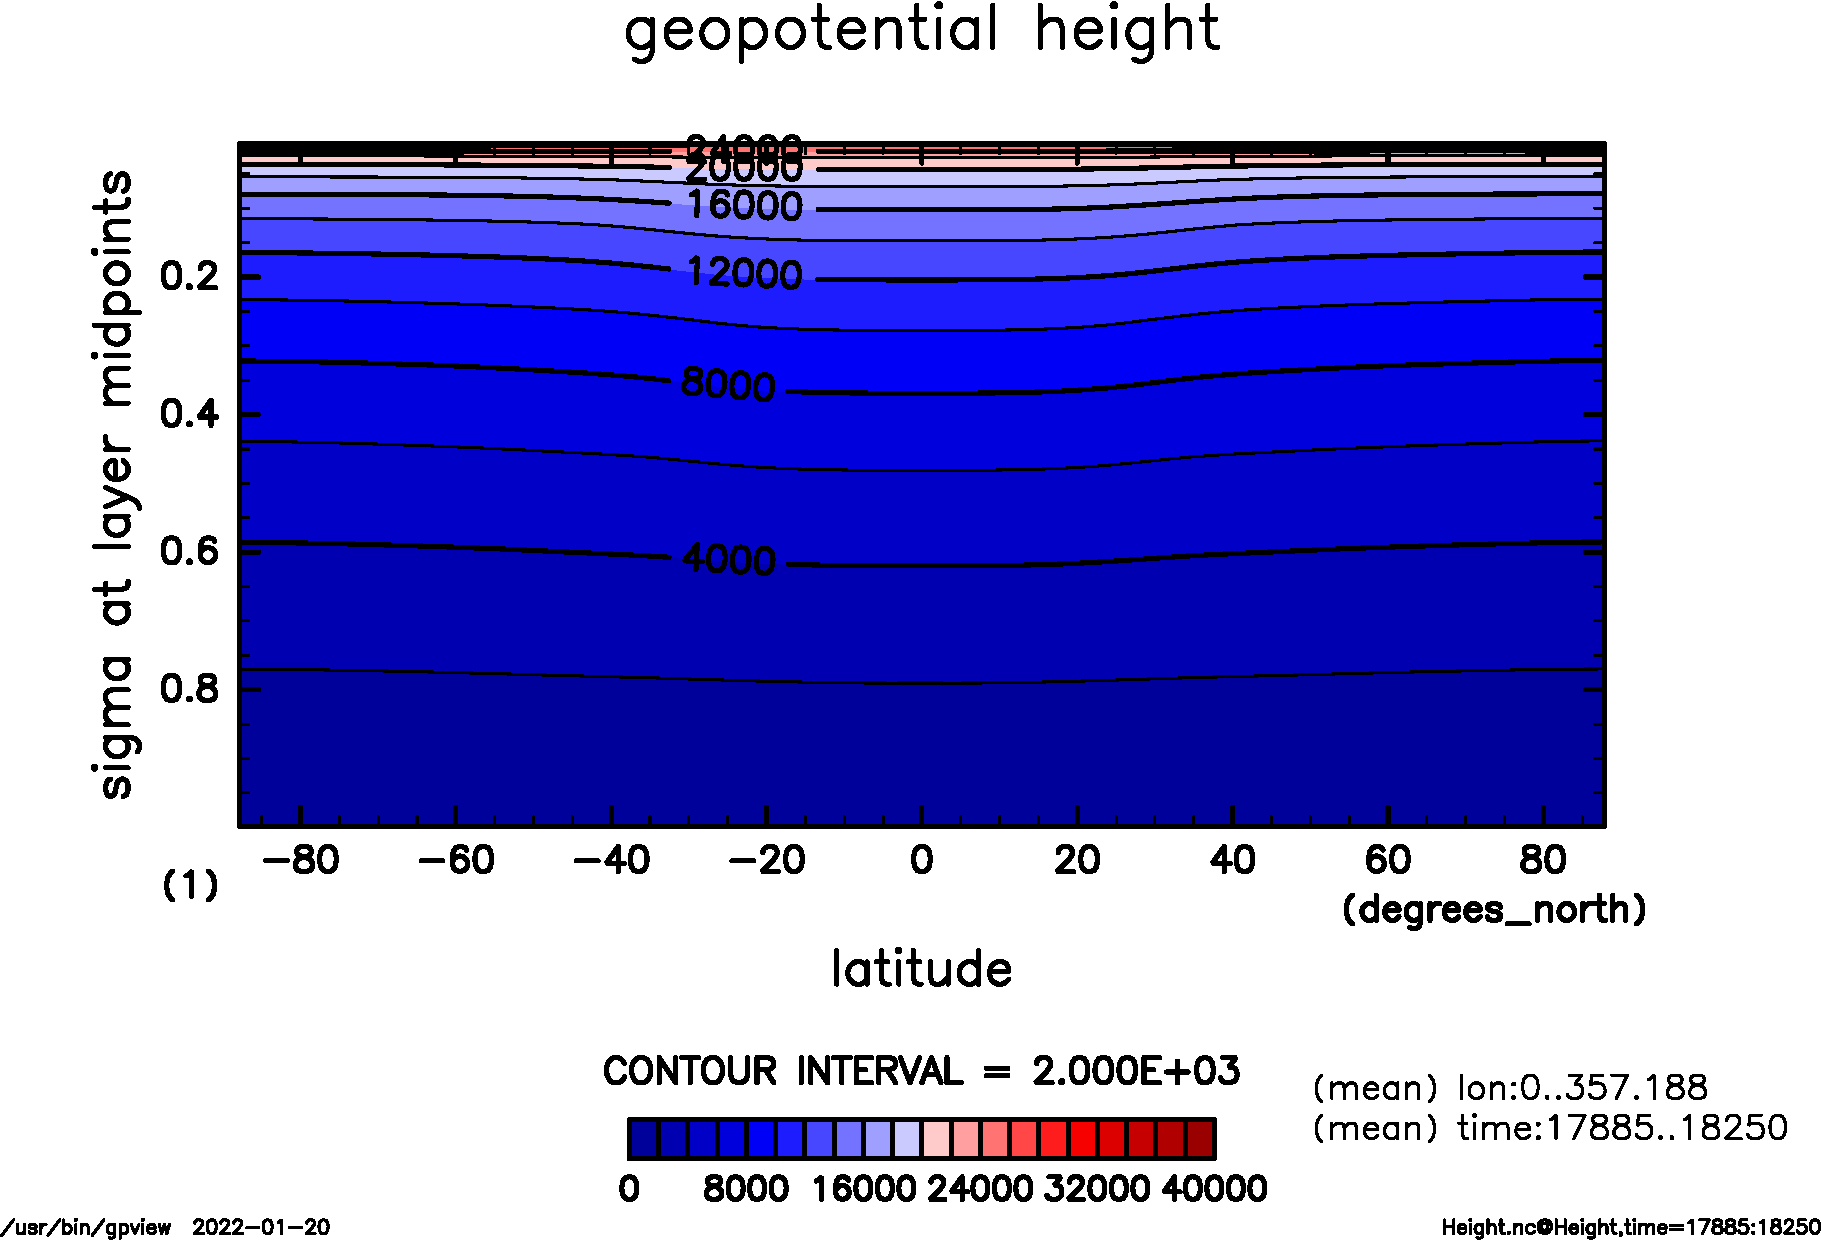
\includegraphics[width=\columnwidth]{S1366/Height,time=17885:18250-crop-rotate.pdf}
		\caption{ジオポテンシャル高度}
	\end{subfigure}
	\caption{
		\(S=1366\hmu{W/m^2}\) の結果
	}
\end{figure}

\begin{figure}[t]
	\centering
	\begin{subfigure}{.4\textwidth}
		\centering
		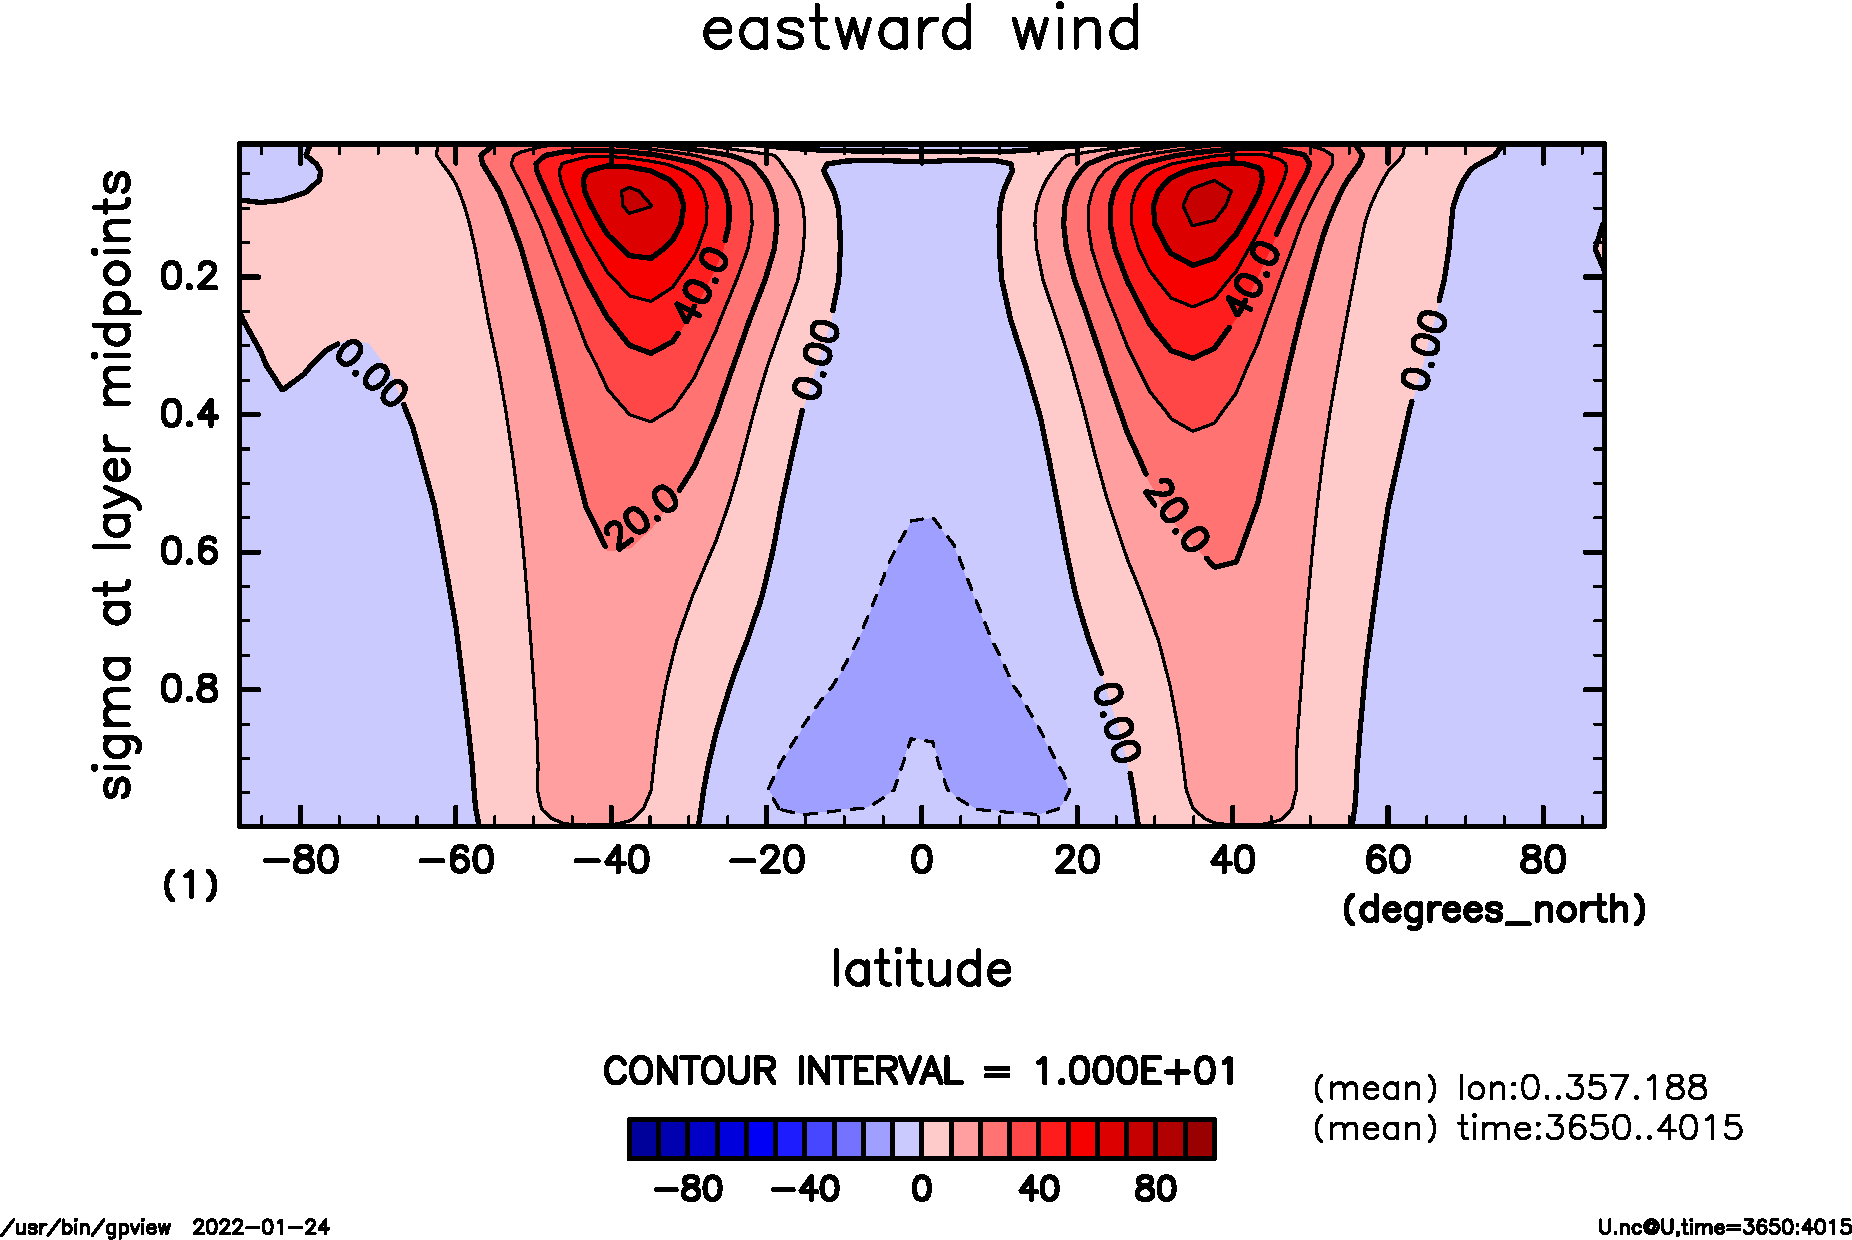
\includegraphics[width=\columnwidth]{S1500/U,time=3650:4015-crop-rotate.pdf}
		\caption{東西風}
	\end{subfigure}
	\begin{subfigure}{.4\textwidth}
		\centering
		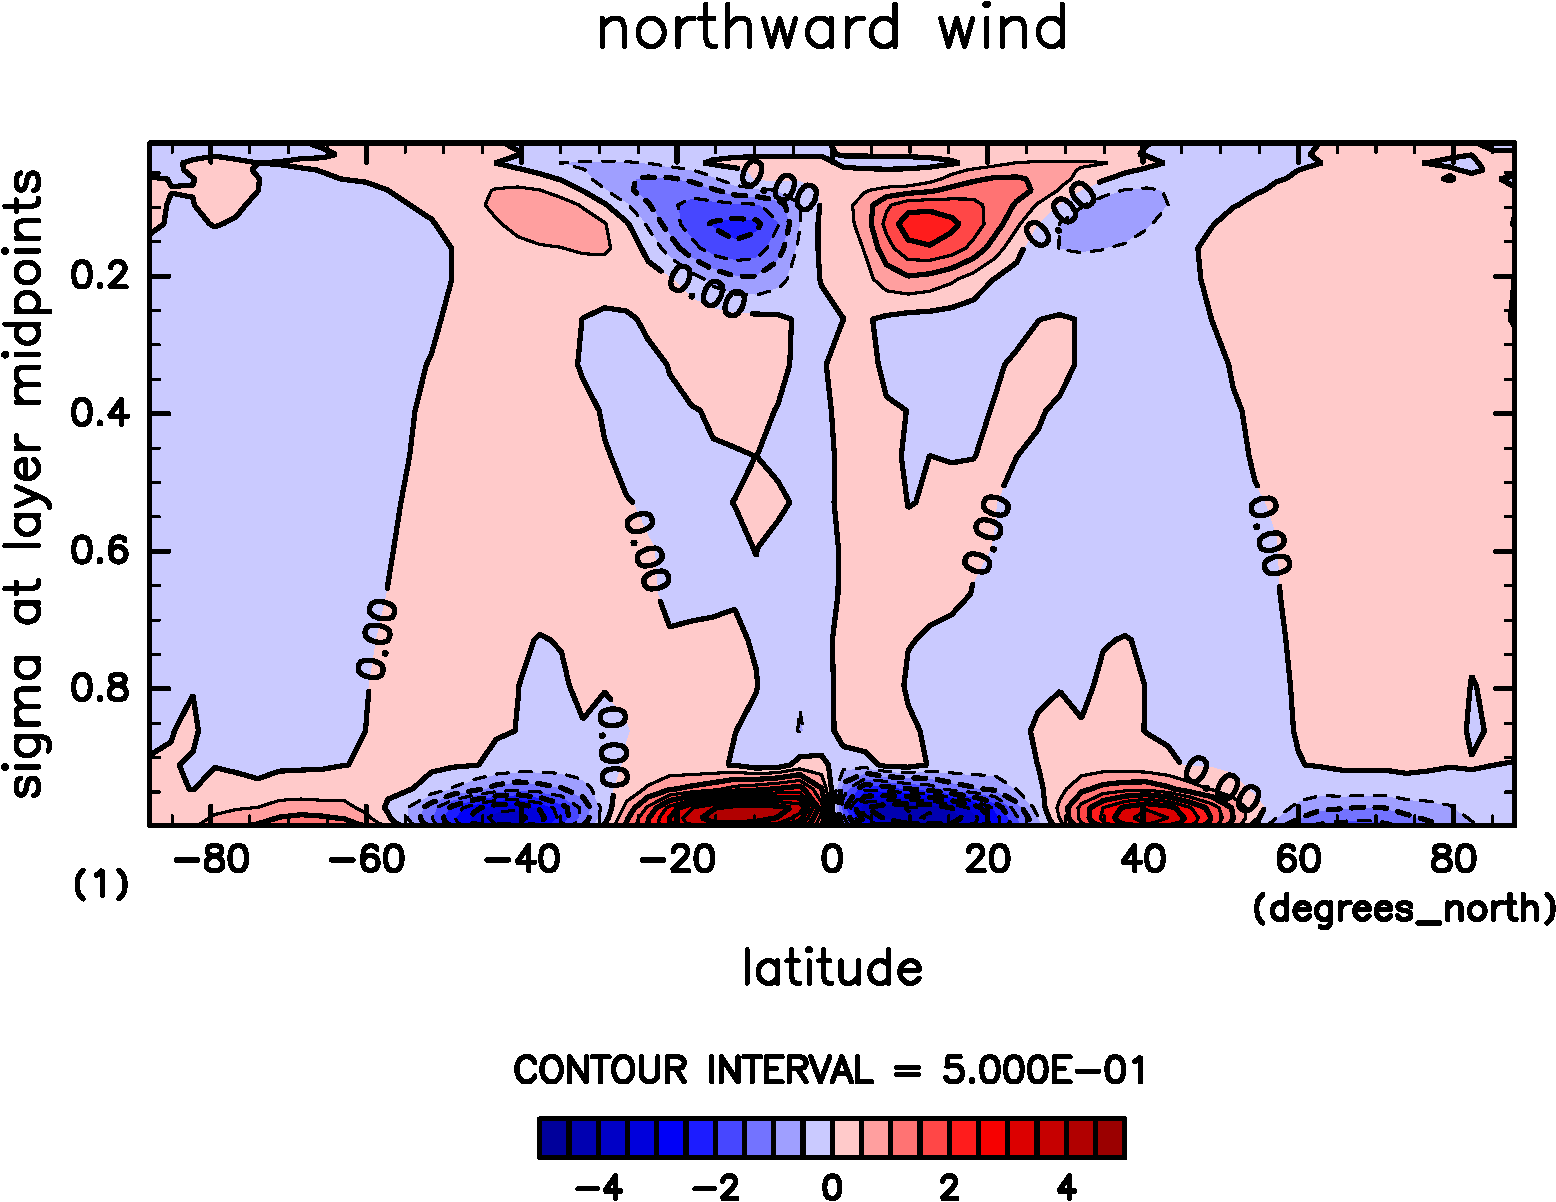
\includegraphics[width=\columnwidth]{S1500/V,time=3650:4015-crop-rotate.pdf}
		\caption{南北風}
	\end{subfigure}
	\begin{subfigure}{.4\textwidth}
		\centering
		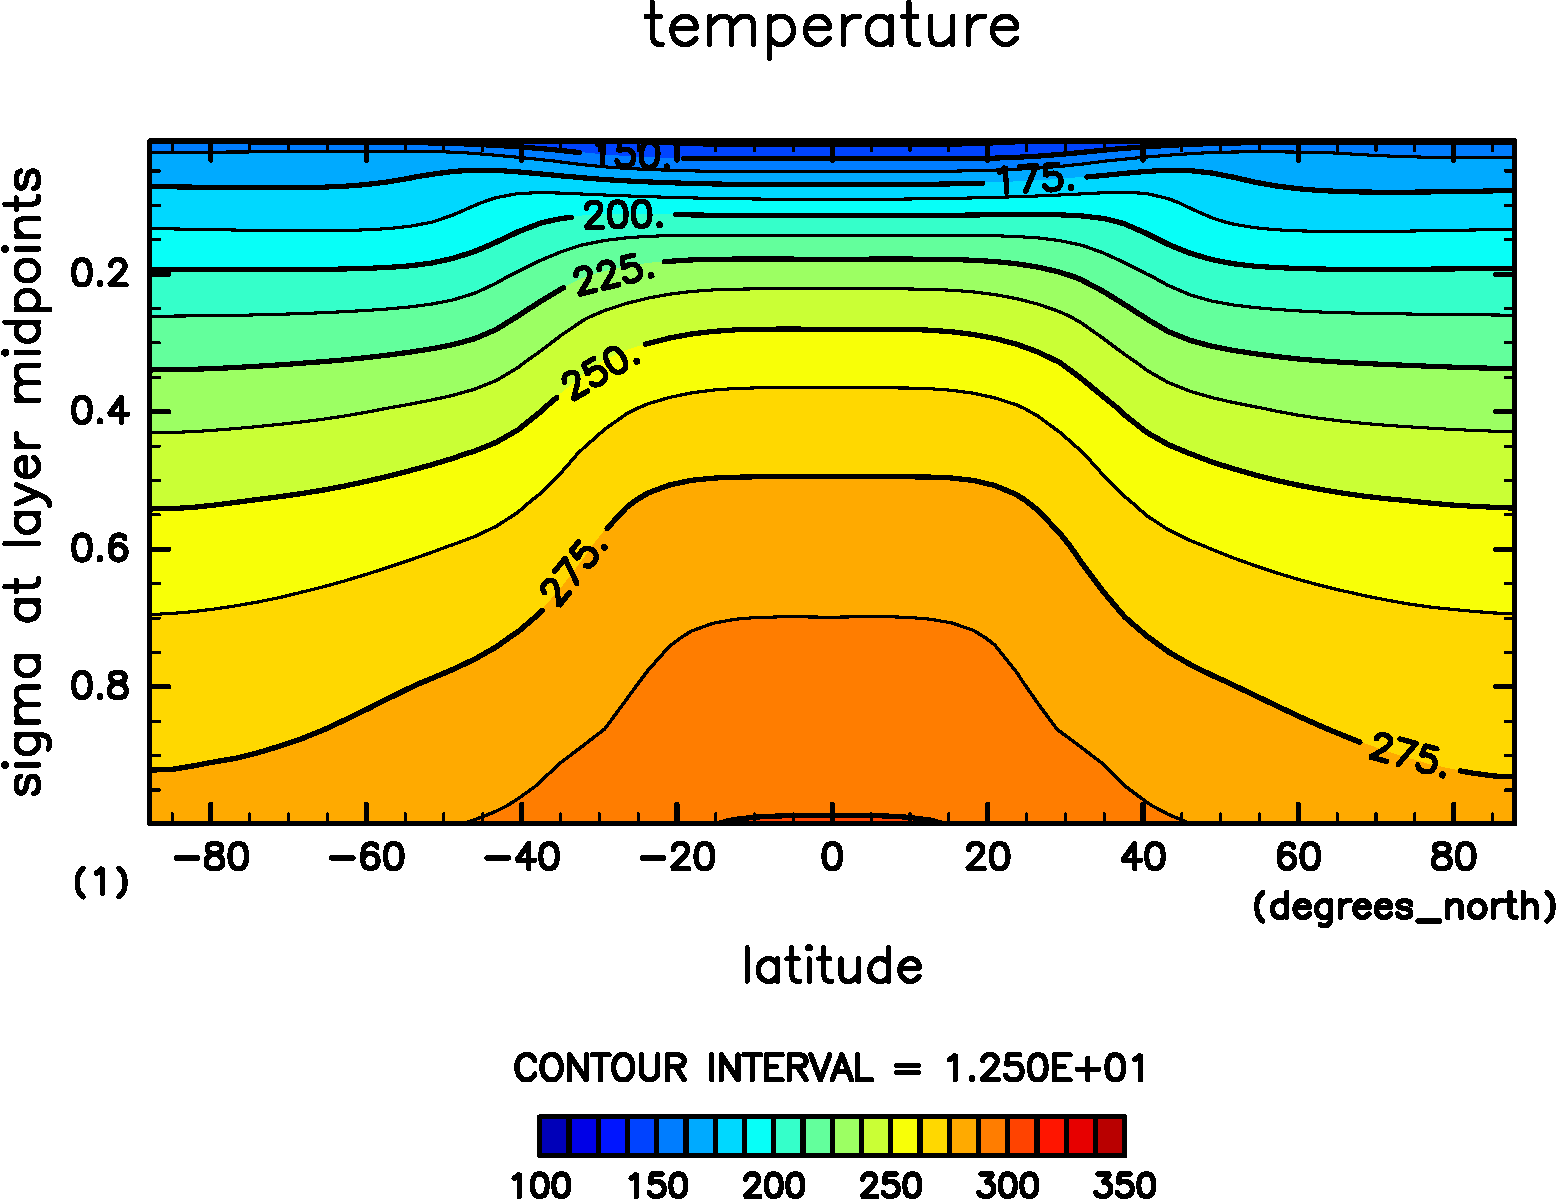
\includegraphics[width=\columnwidth]{S1500/Temp,time=3650:4015-crop-rotate.pdf}
		\caption{気温分布}
	\end{subfigure}
	\begin{subfigure}{.4\textwidth}
		\centering
		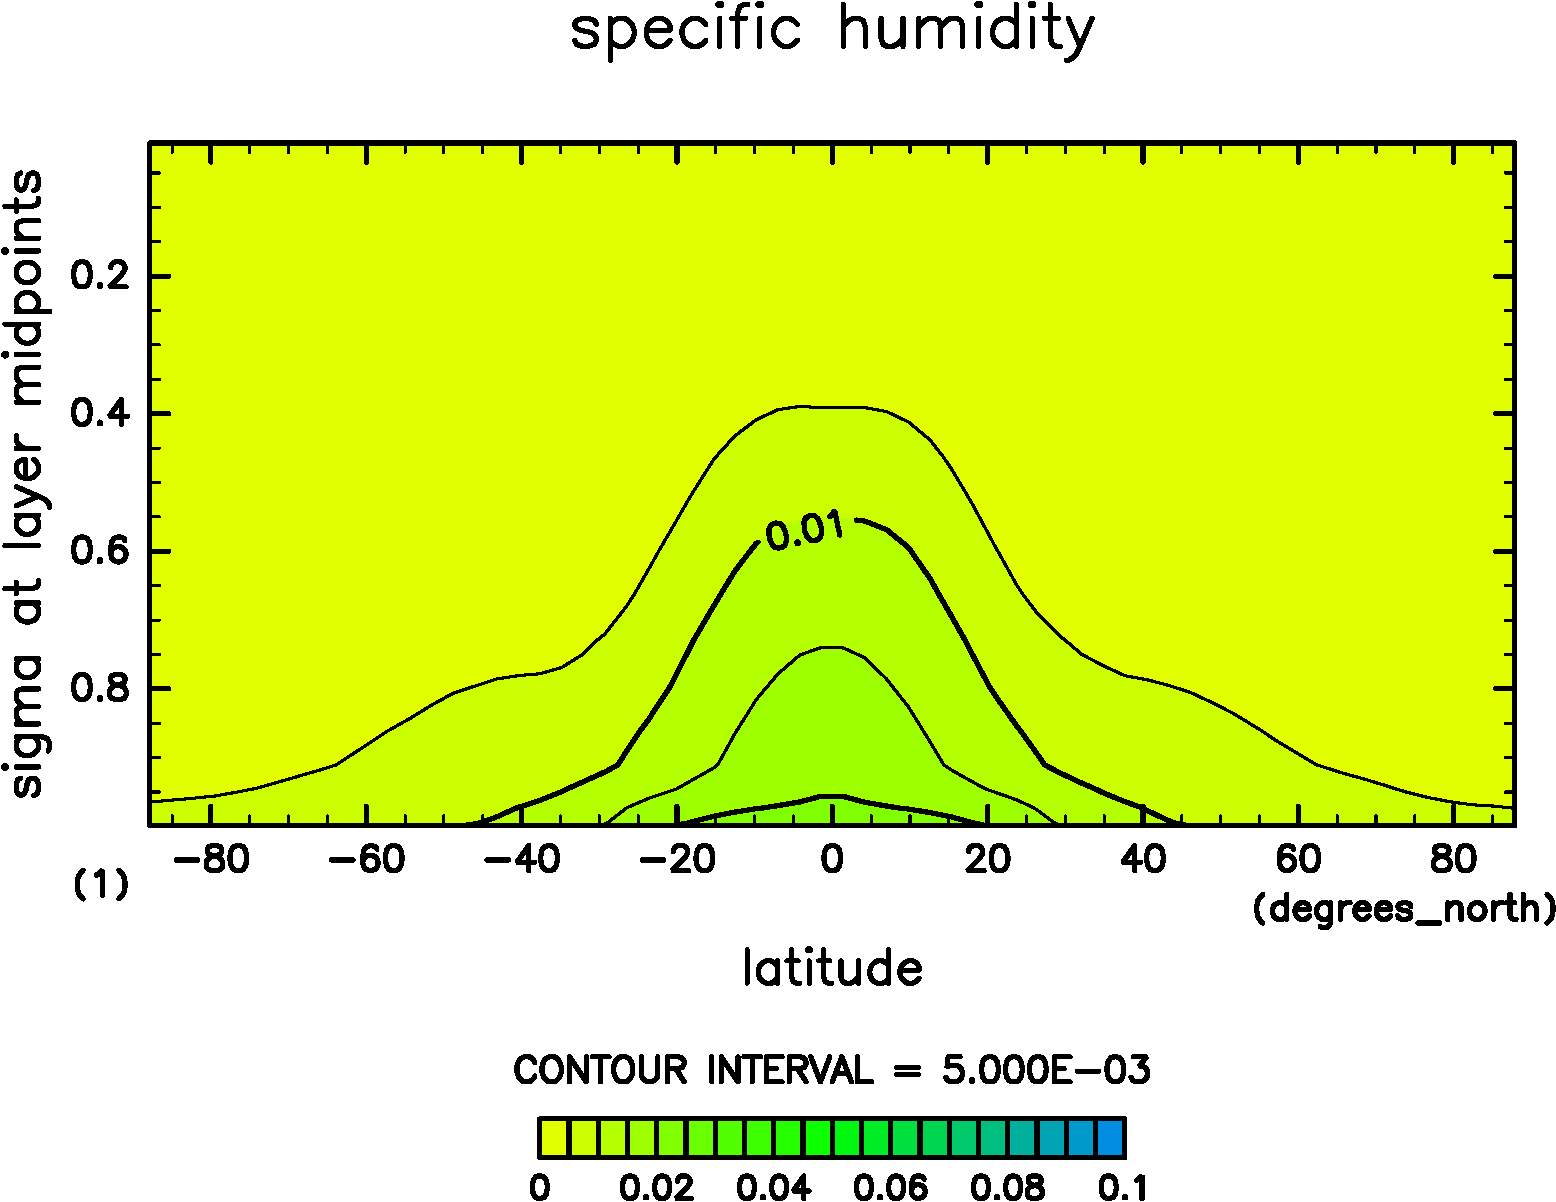
\includegraphics[width=\columnwidth]{S1500/QH2OVap,time=3650:4015-crop-rotate.pdf}
		\caption{比湿}
	\end{subfigure}
	\begin{subfigure}{.4\textwidth}
		\centering
		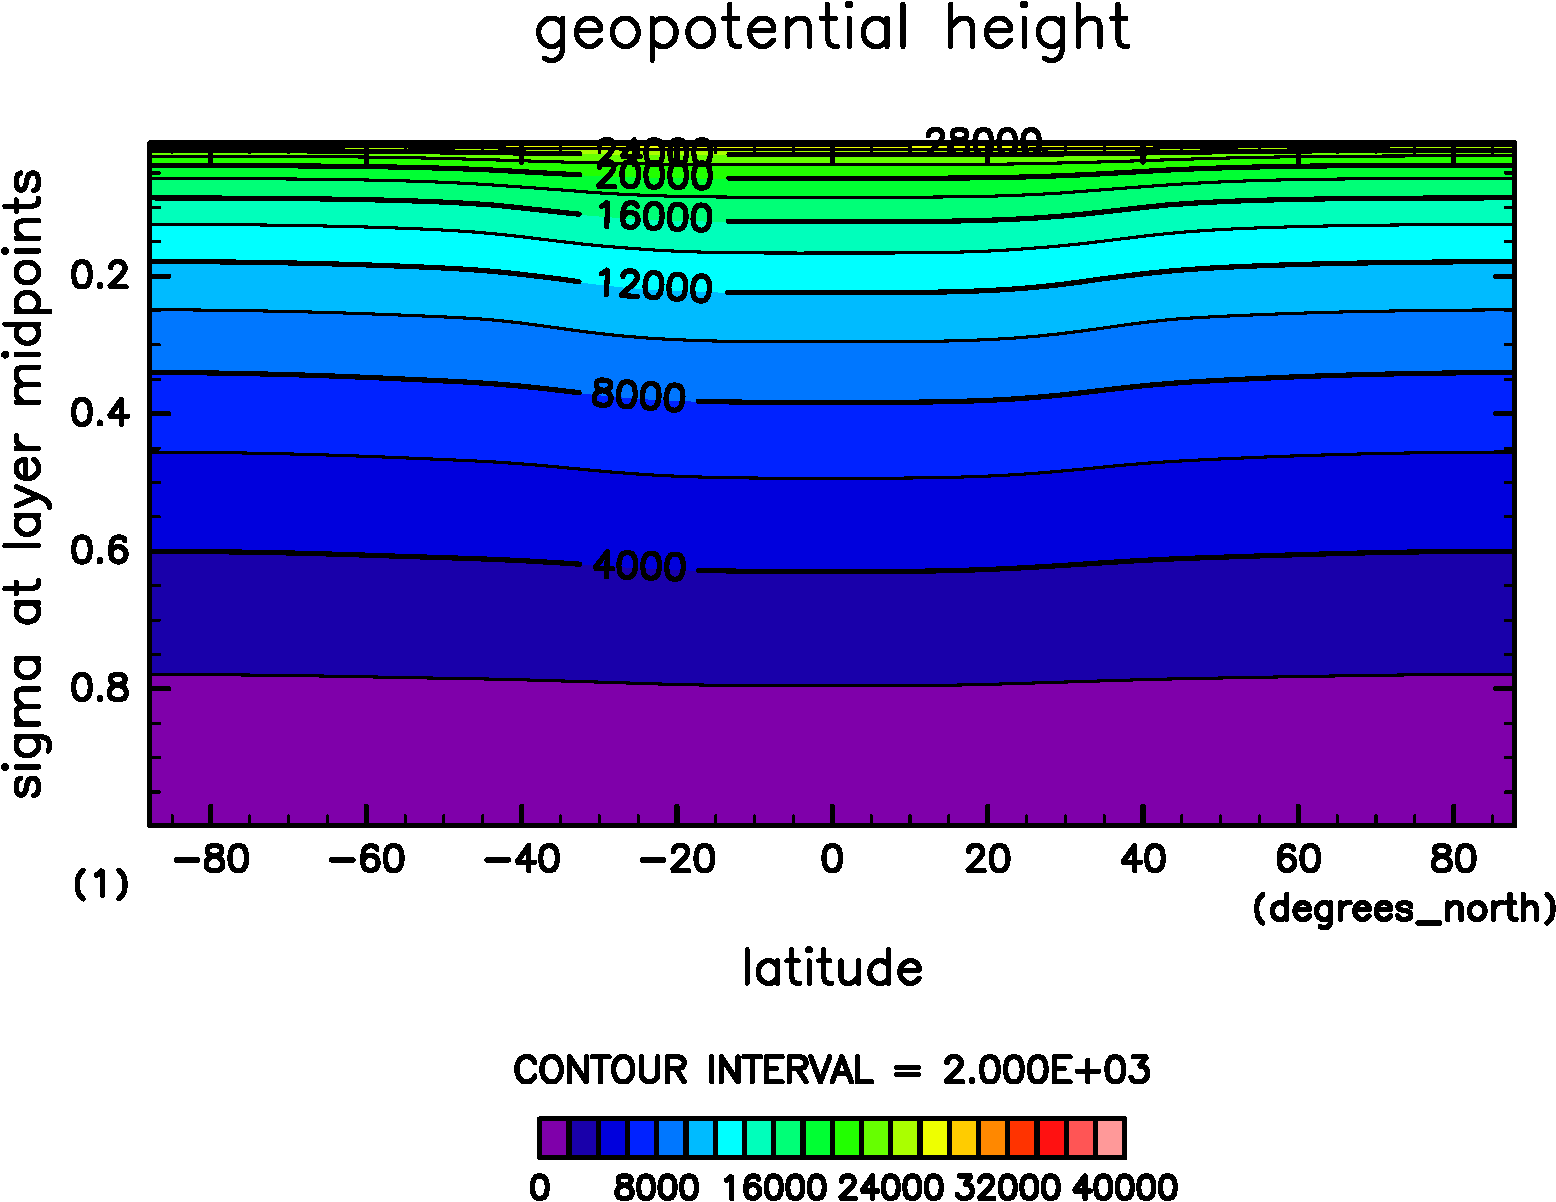
\includegraphics[width=\columnwidth]{S1500/Height,time=3650:4015-crop-rotate.pdf}
		\caption{ジオポテンシャル高度}
	\end{subfigure}
	\caption{
		\(S=1500\hmu{W/m^2}\) の結果
	}
\end{figure}

\begin{figure}[t]
	\centering
	\begin{subfigure}{.4\textwidth}
		\centering
		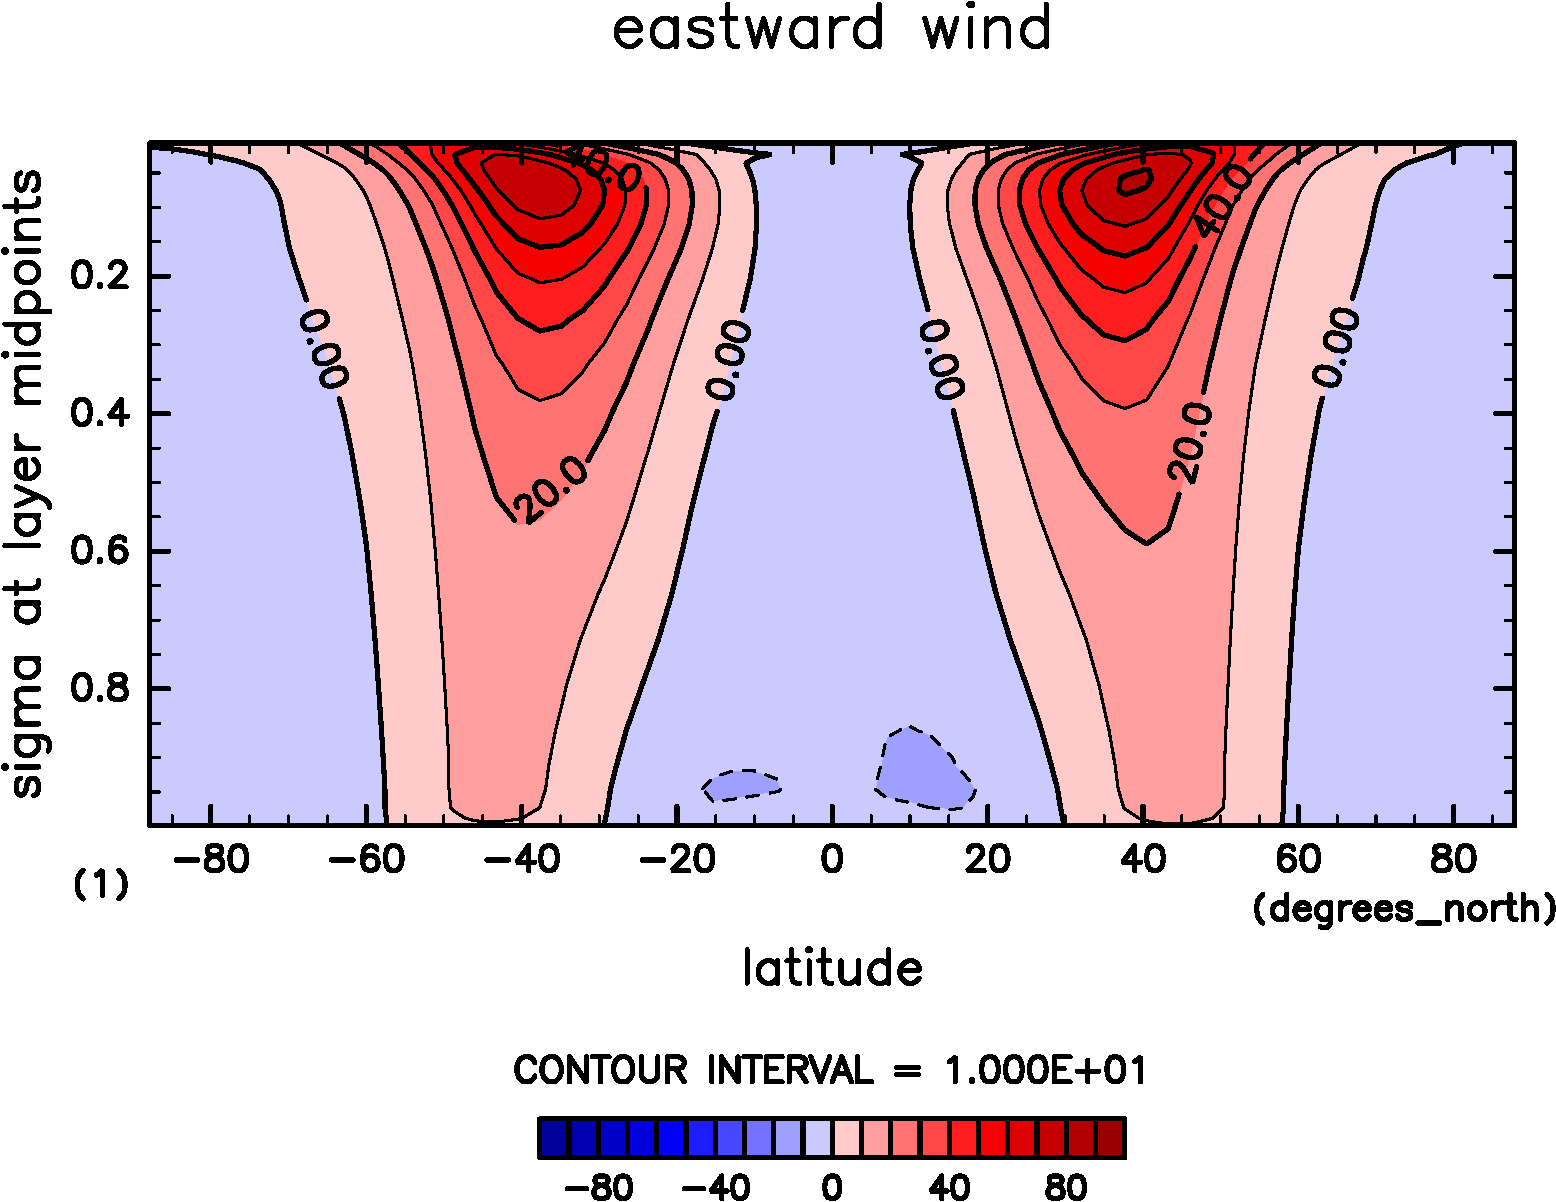
\includegraphics[width=\columnwidth]{S1600/U,time=3650:4015-crop-rotate.pdf}
		\caption{東西風}
	\end{subfigure}
	\begin{subfigure}{.4\textwidth}
		\centering
		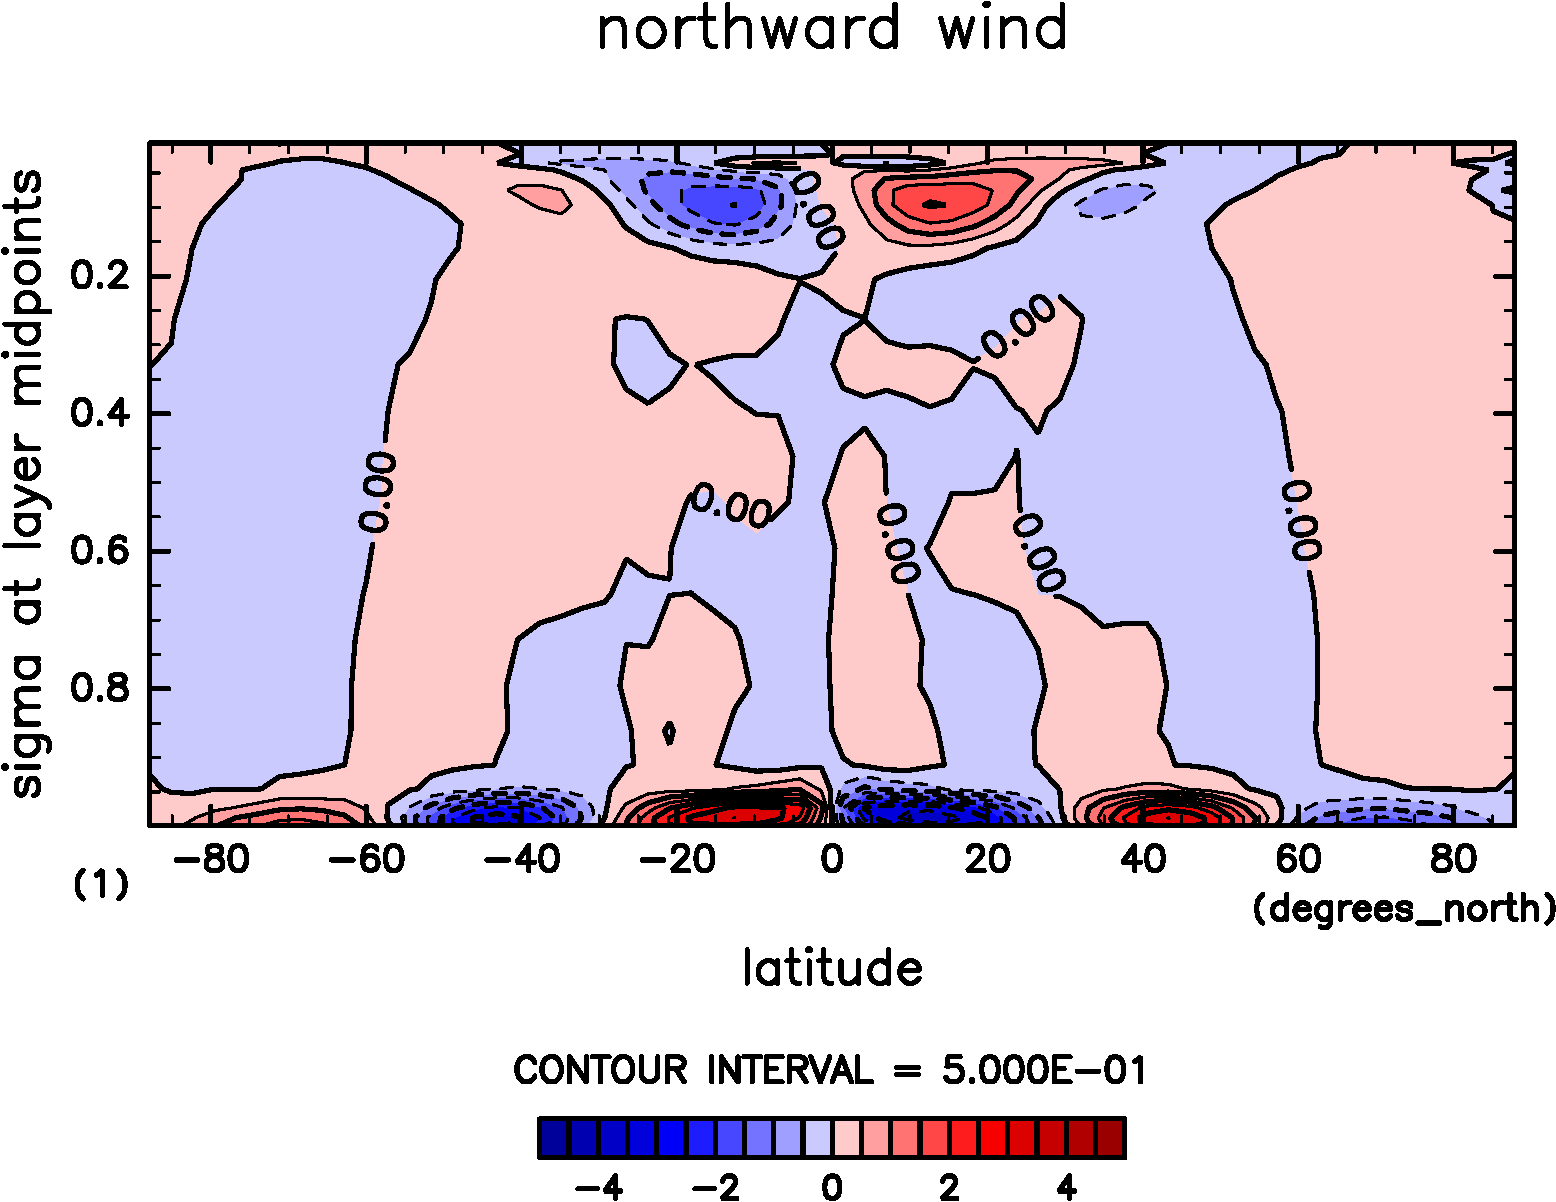
\includegraphics[width=\columnwidth]{S1600/V,time=3650:4015-crop-rotate.pdf}
		\caption{南北風}
	\end{subfigure}
	\begin{subfigure}{.4\textwidth}
		\centering
		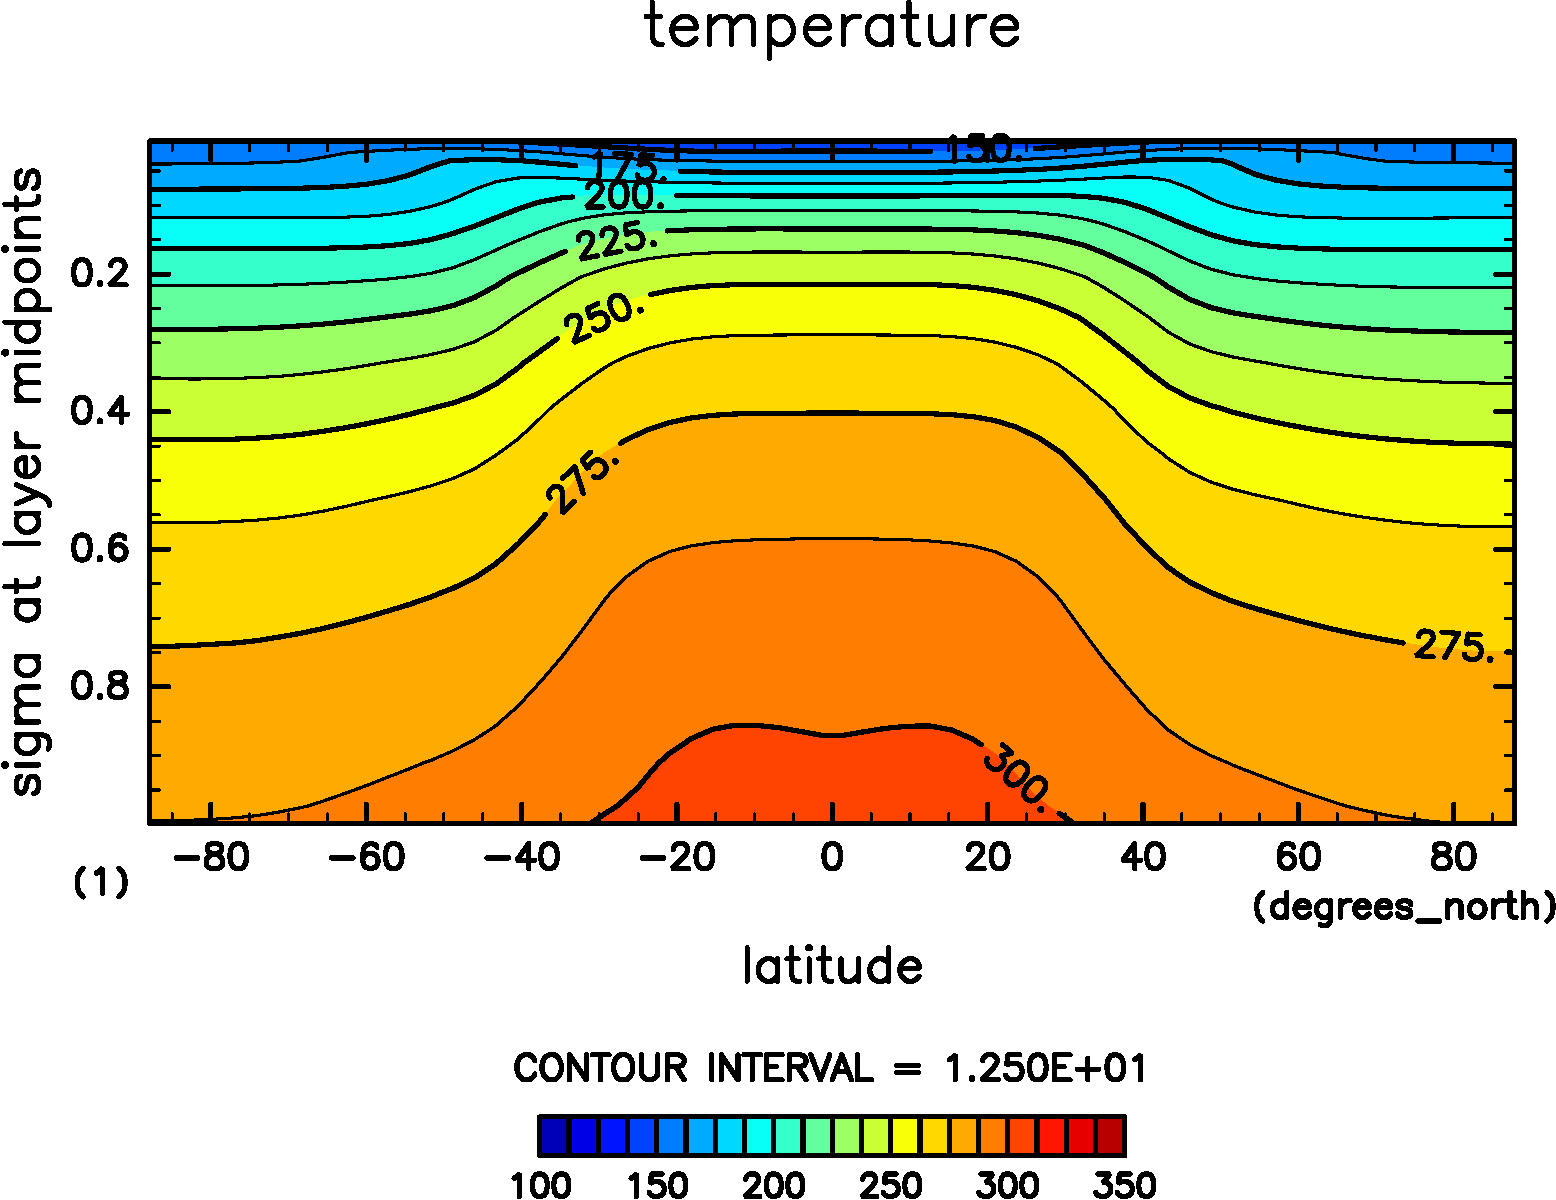
\includegraphics[width=\columnwidth]{S1600/Temp,time=3650:4015-crop-rotate.pdf}
		\caption{気温分布}
	\end{subfigure}
	\begin{subfigure}{.4\textwidth}
		\centering
		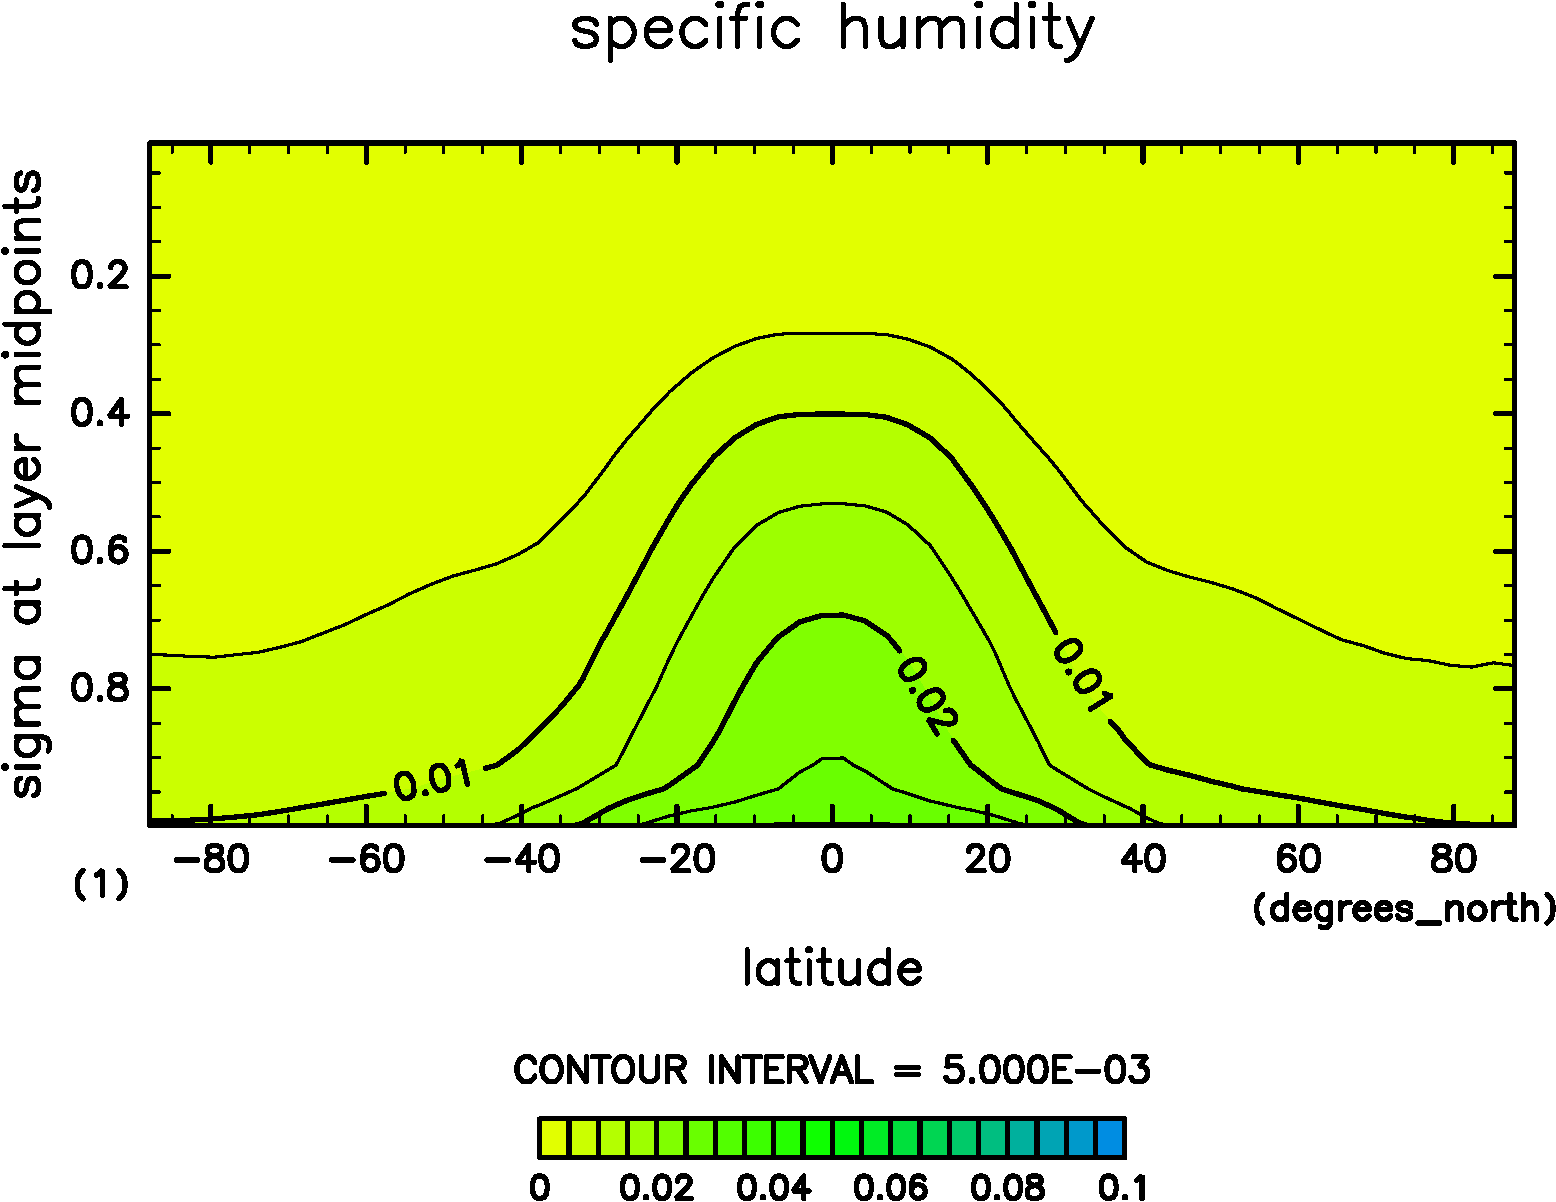
\includegraphics[width=\columnwidth]{S1600/QH2OVap,time=3650:4015-crop-rotate.pdf}
		\caption{比湿}
	\end{subfigure}
	\begin{subfigure}{.4\textwidth}
		\centering
		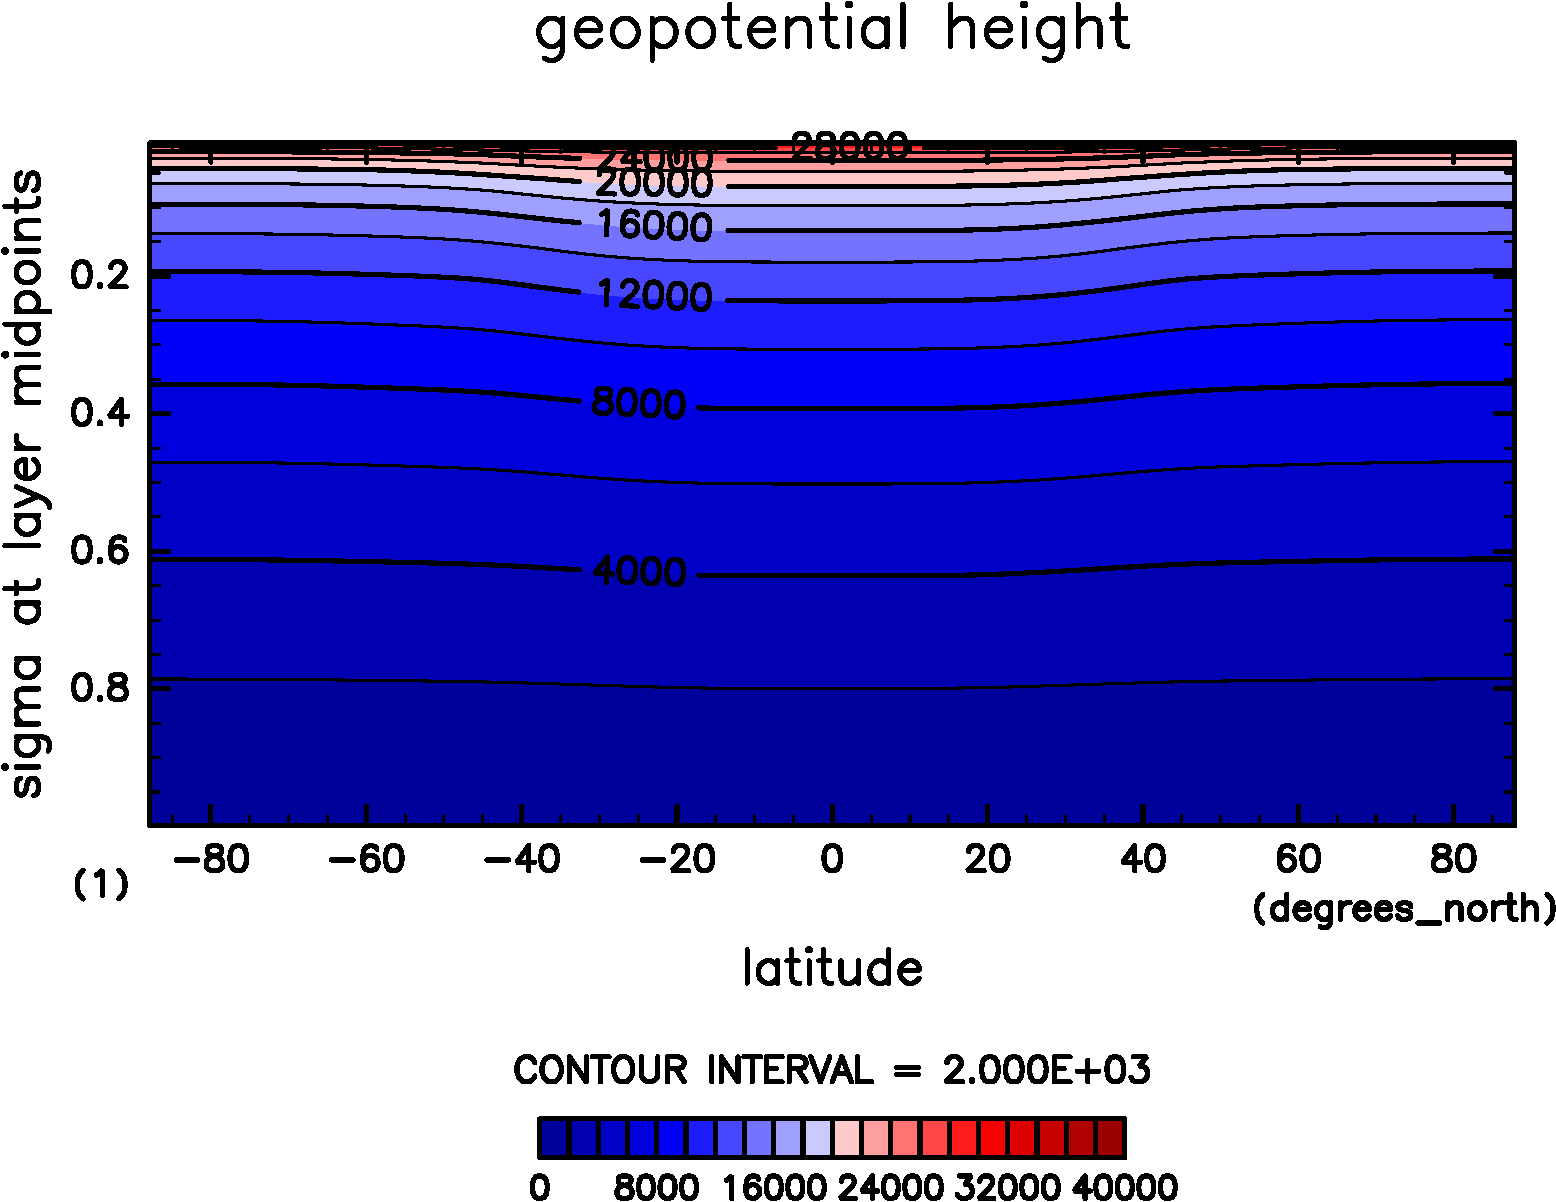
\includegraphics[width=\columnwidth]{S1600/Height,time=3650:4015-crop-rotate.pdf}
		\caption{ジオポテンシャル高度}
	\end{subfigure}
	\caption{
		\(S=1600\hmu{W/m^2}\) の結果
	}
\end{figure}

\begin{figure}[t]
	\centering
	\begin{subfigure}{.4\textwidth}
		\centering
		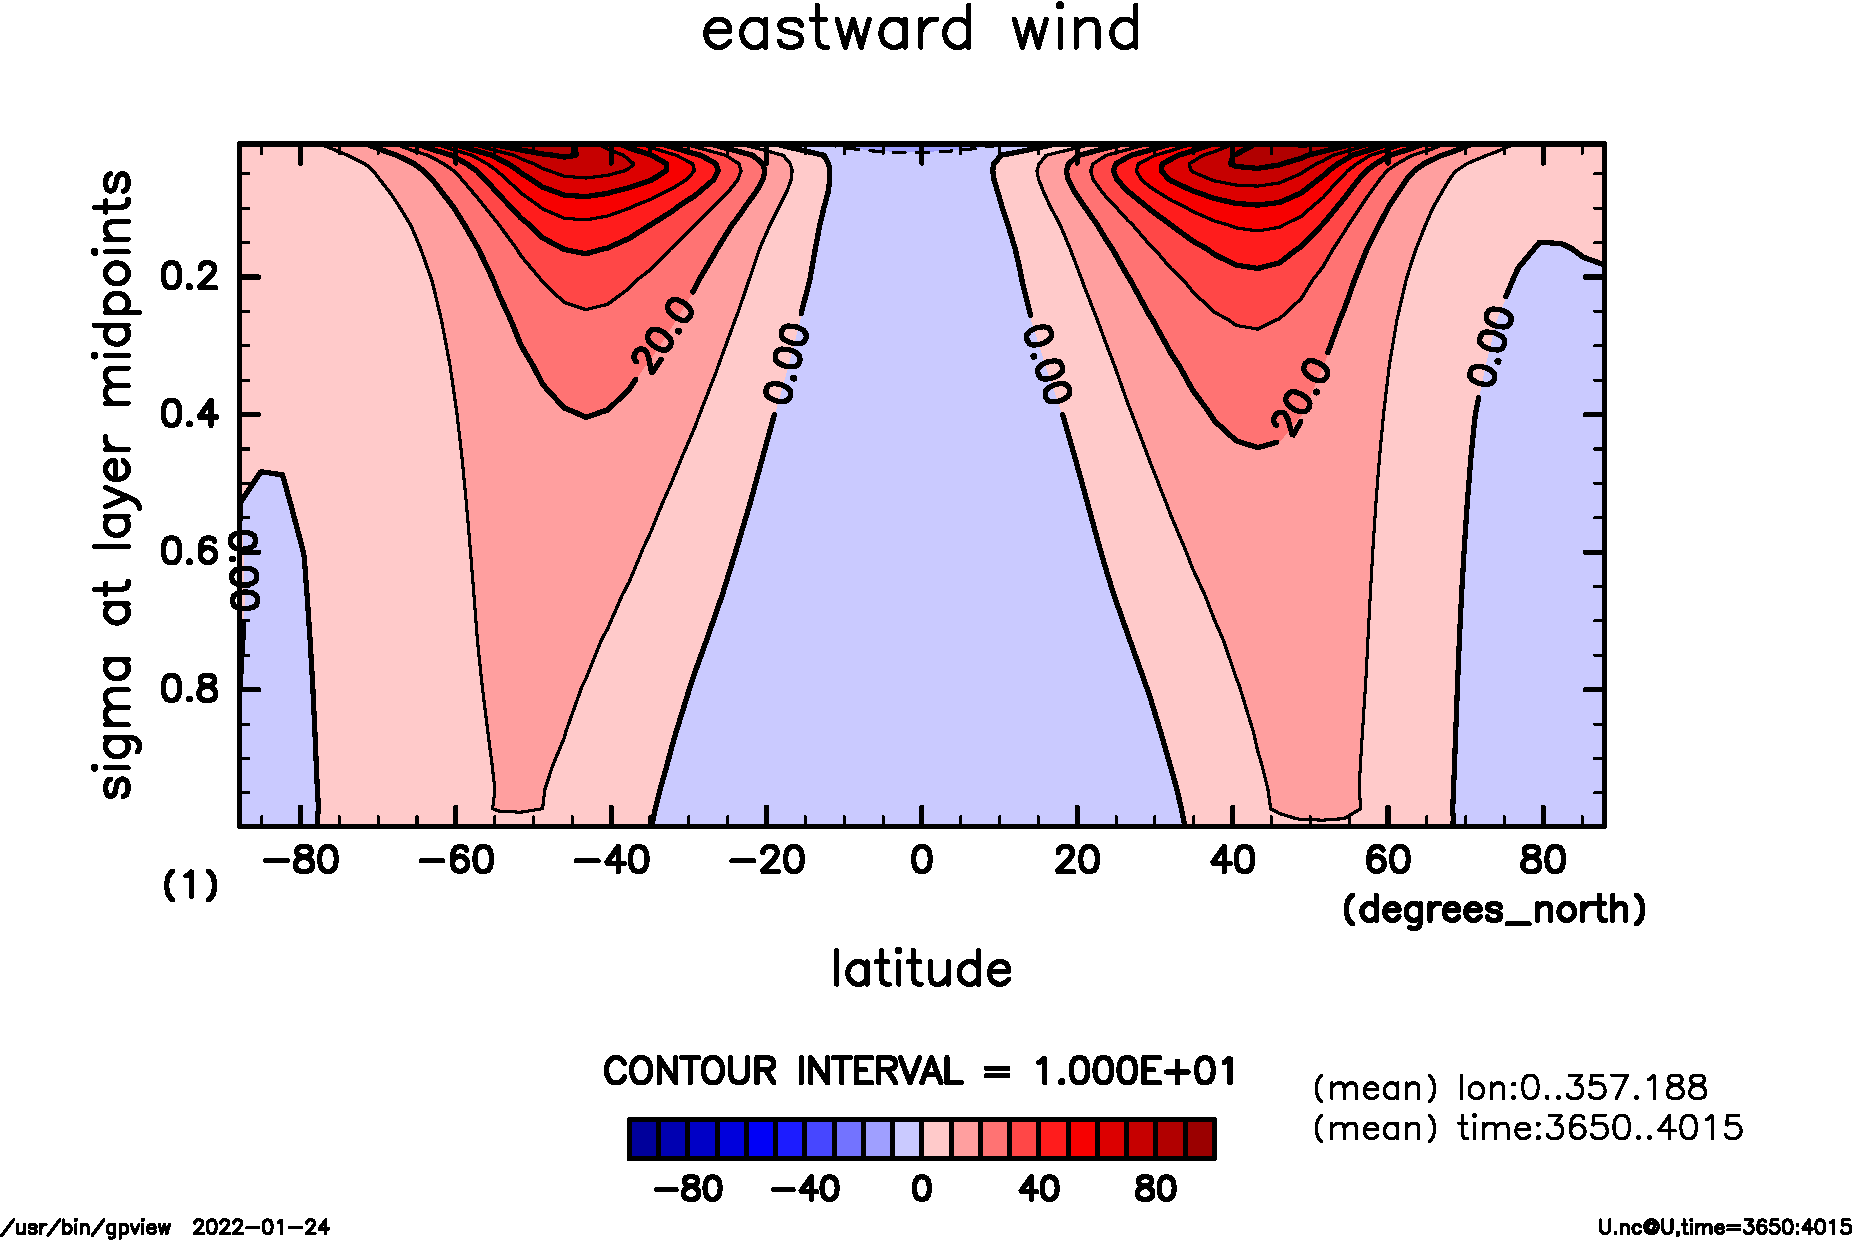
\includegraphics[width=\columnwidth]{S1800/U,time=3650:4015-crop-rotate.pdf}
		\caption{東西風}
	\end{subfigure}
	\begin{subfigure}{.4\textwidth}
		\centering
		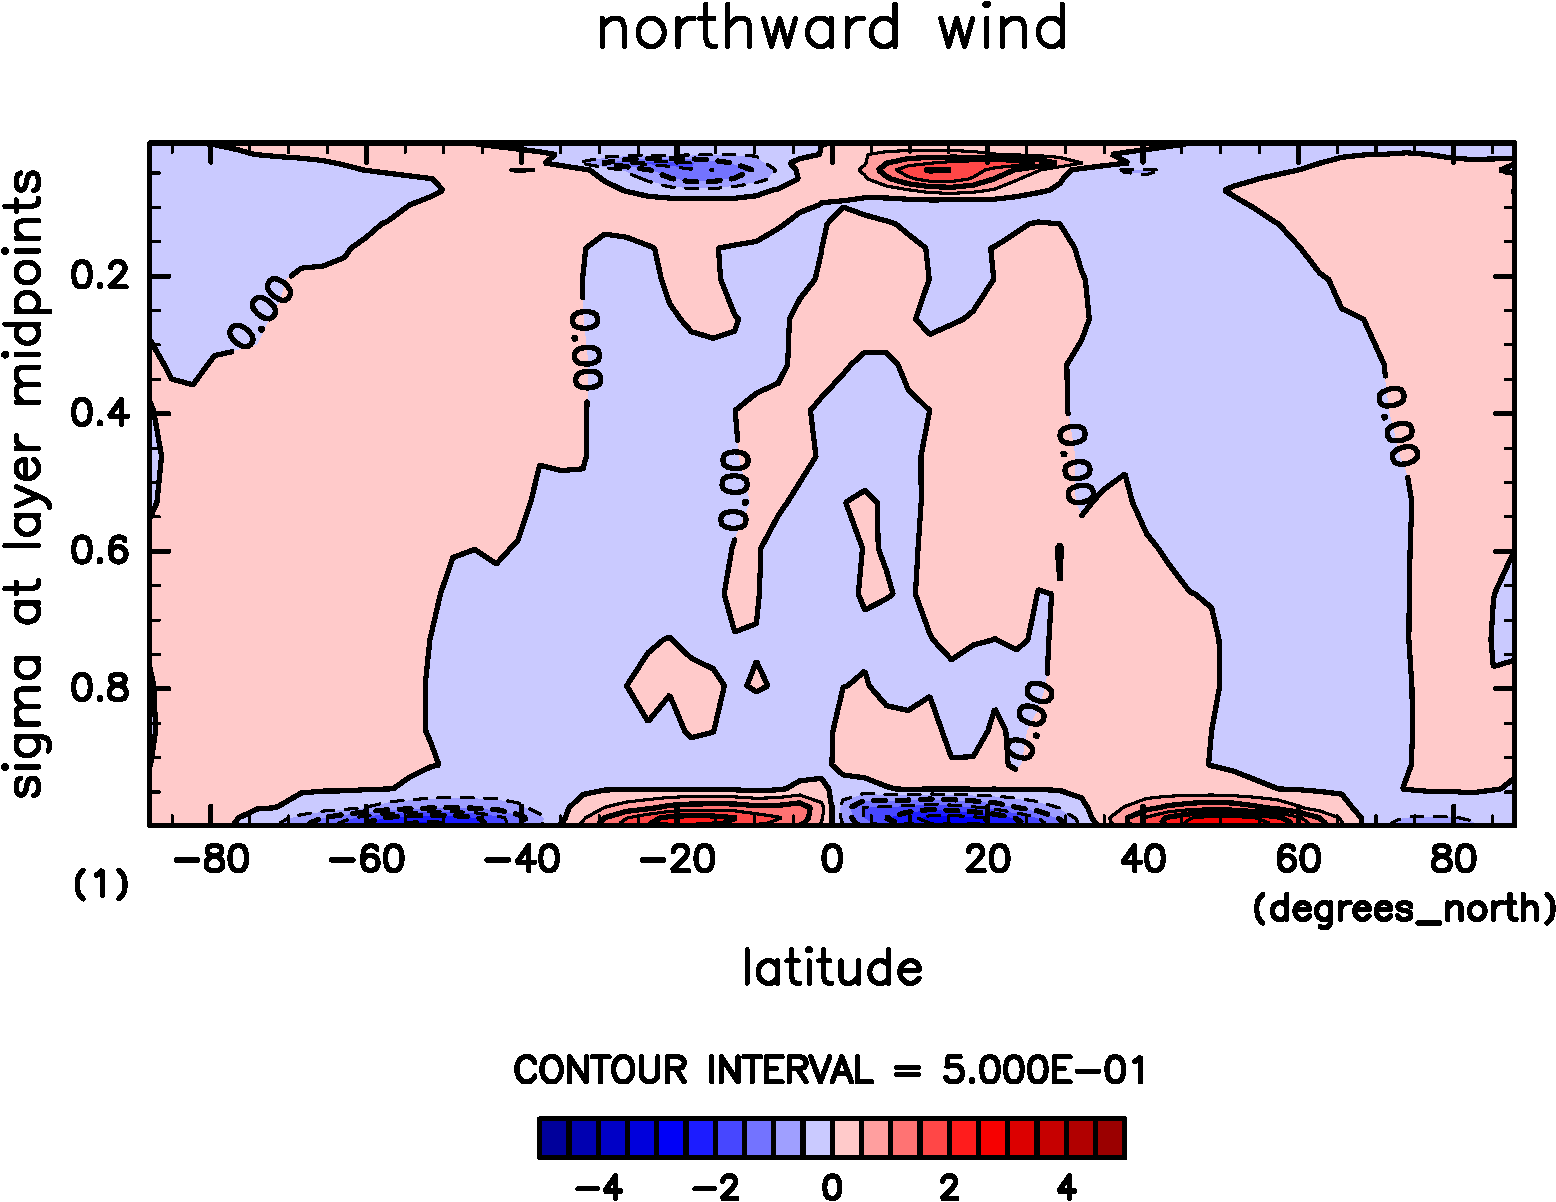
\includegraphics[width=\columnwidth]{S1800/V,time=3650:4015-crop-rotate.pdf}
		\caption{南北風}
	\end{subfigure}
	\begin{subfigure}{.4\textwidth}
		\centering
		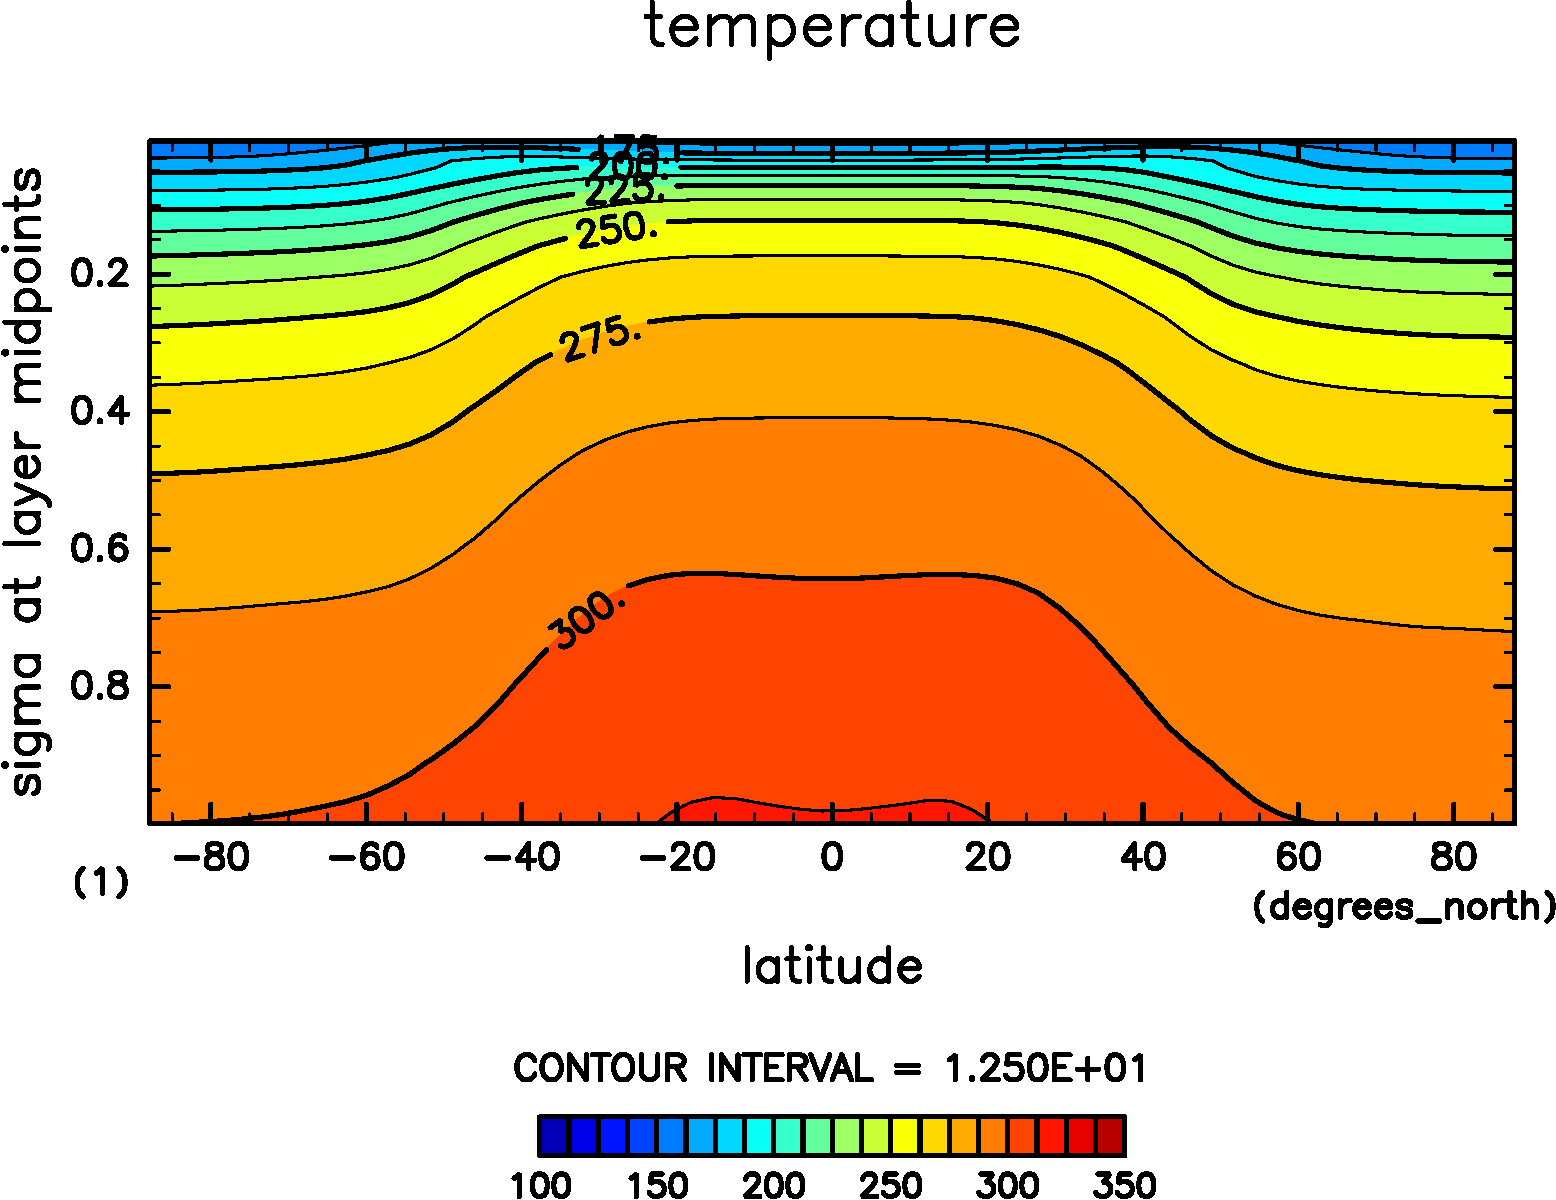
\includegraphics[width=\columnwidth]{S1800/Temp,time=3650:4015-crop-rotate.pdf}
		\caption{気温分布}
	\end{subfigure}
	\begin{subfigure}{.4\textwidth}
		\centering
		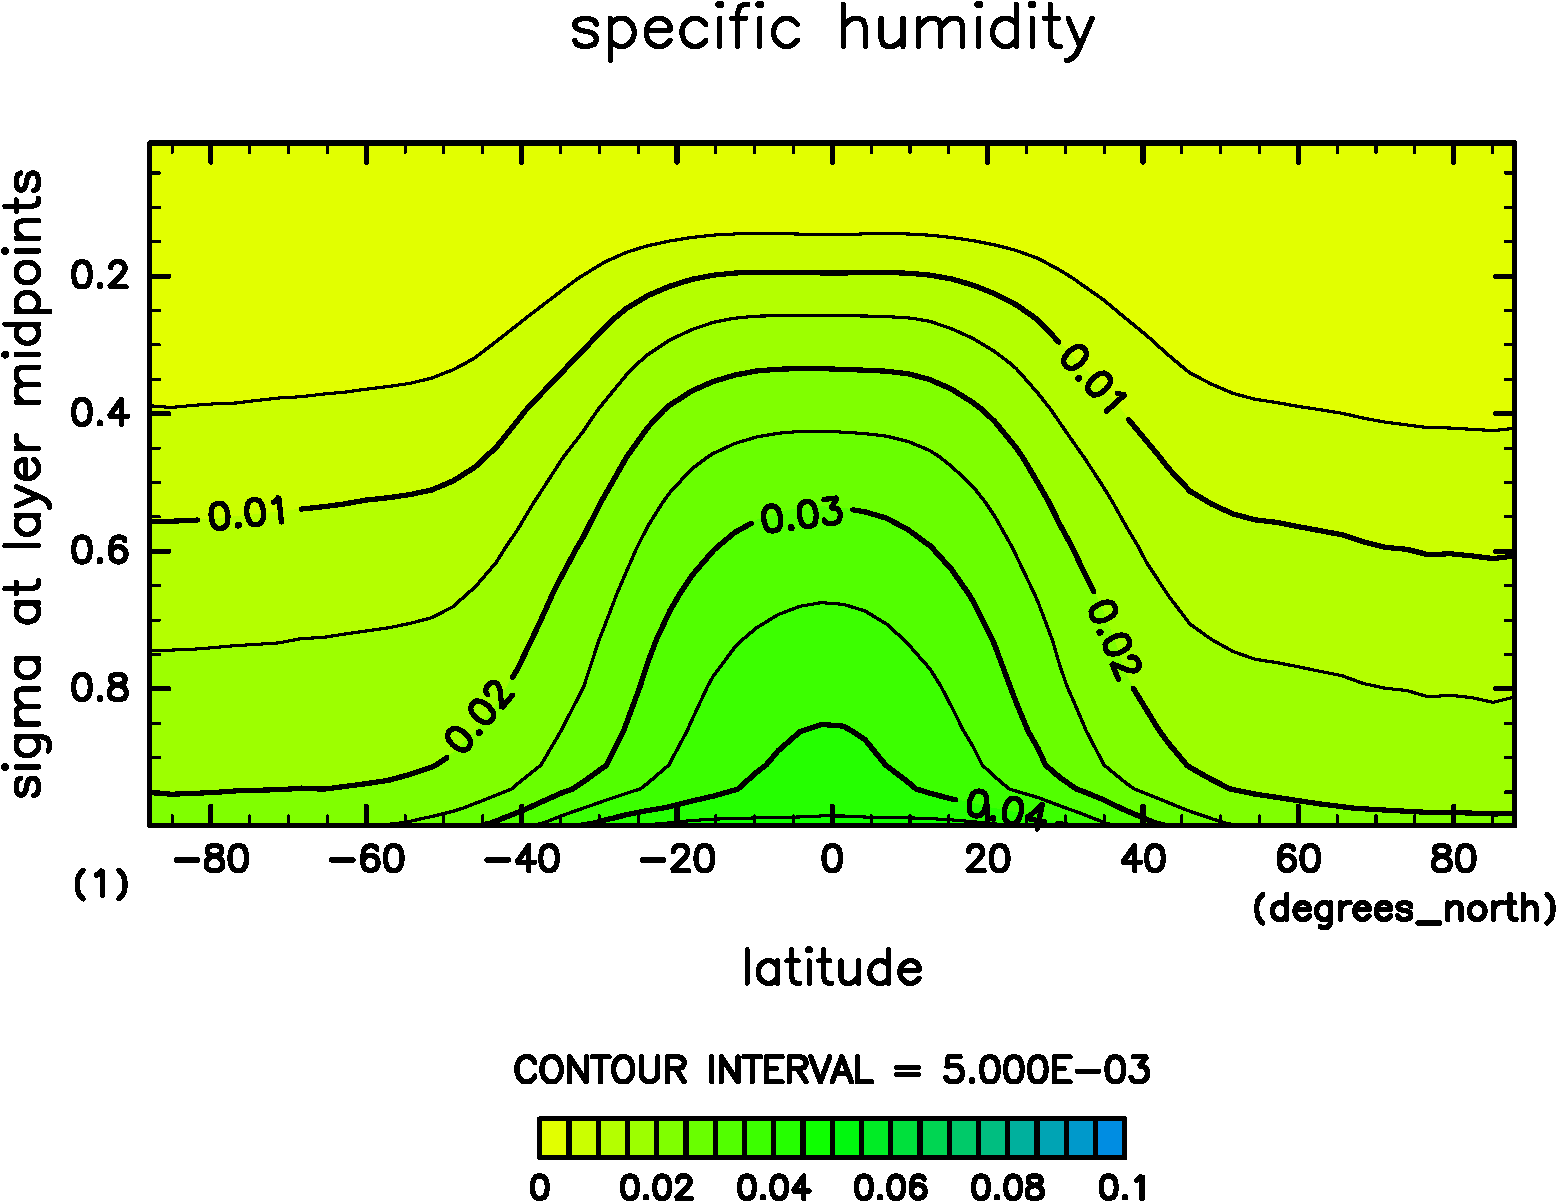
\includegraphics[width=\columnwidth]{S1800/QH2OVap,time=3650:4015-crop-rotate.pdf}
		\caption{比湿}
	\end{subfigure}
	\begin{subfigure}{.4\textwidth}
		\centering
		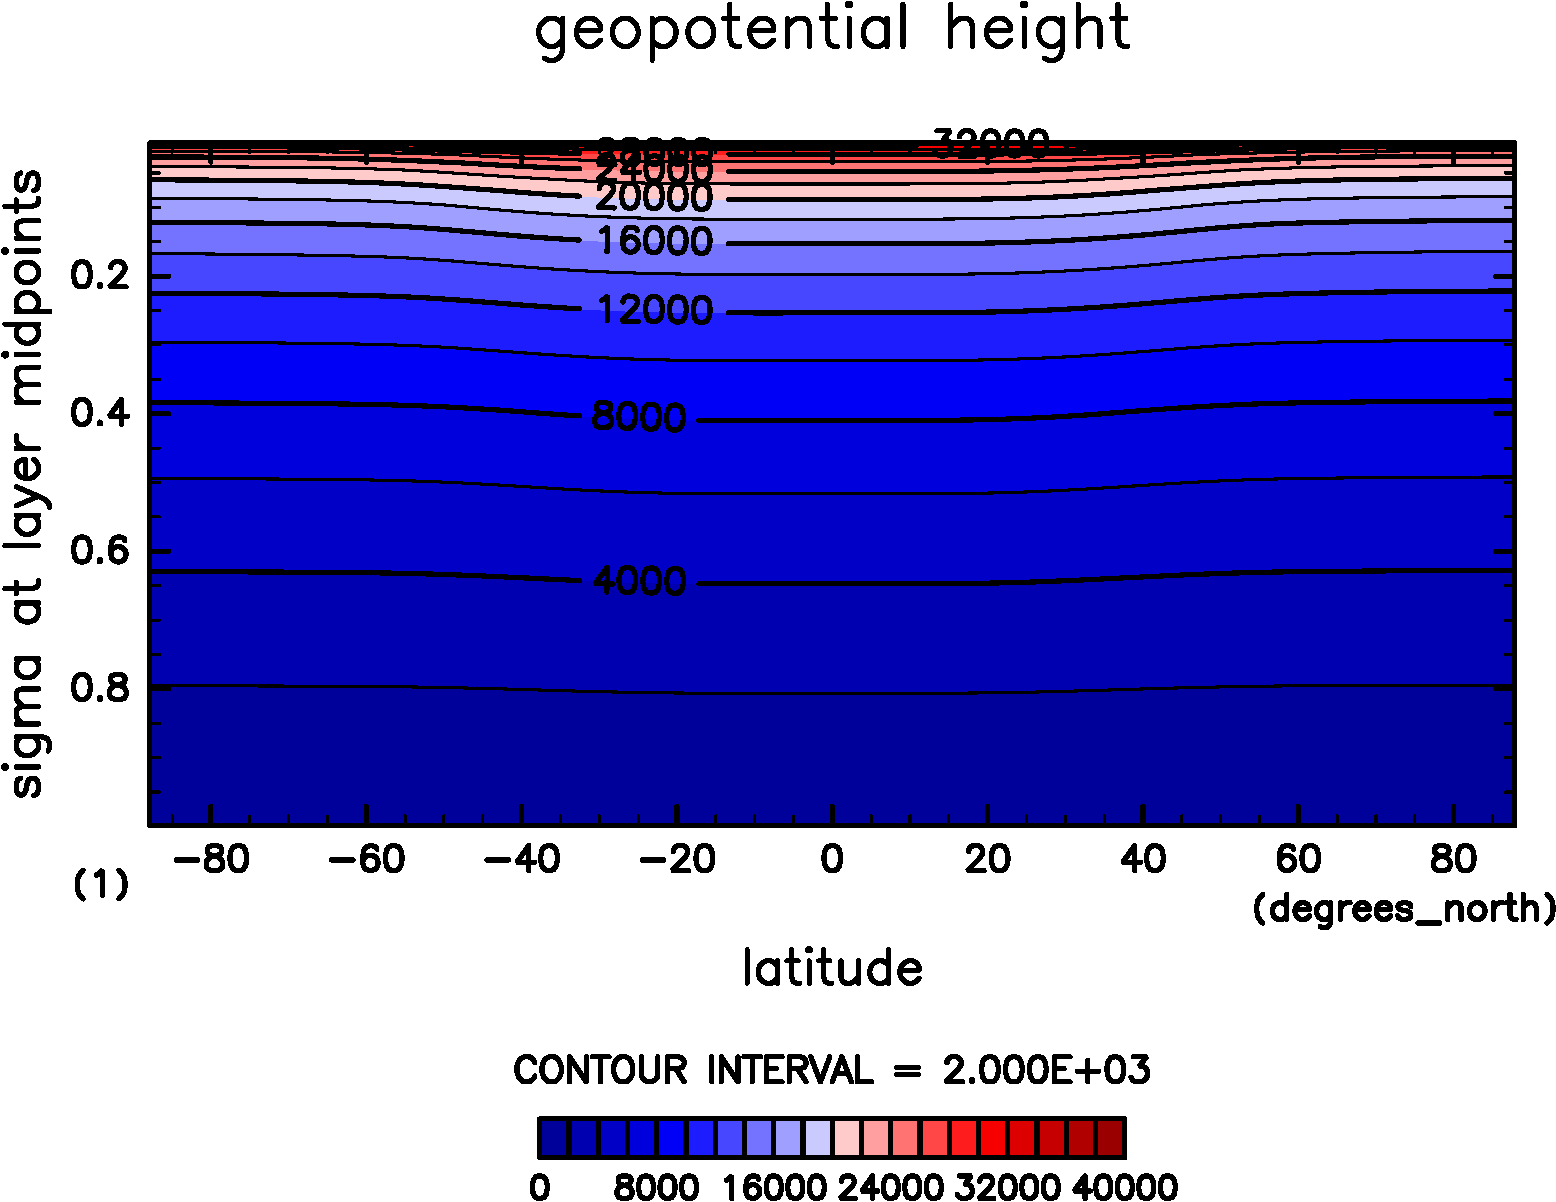
\includegraphics[width=\columnwidth]{S1800/Height,time=3650:4015-crop-rotate.pdf}
		\caption{ジオポテンシャル高度}
	\end{subfigure}
	\caption{
		\(S=1800\hmu{W/m^2}\) の結果
	}
\end{figure}

\begin{figure}[t]
	\centering
	\begin{subfigure}{.4\textwidth}
		\centering
		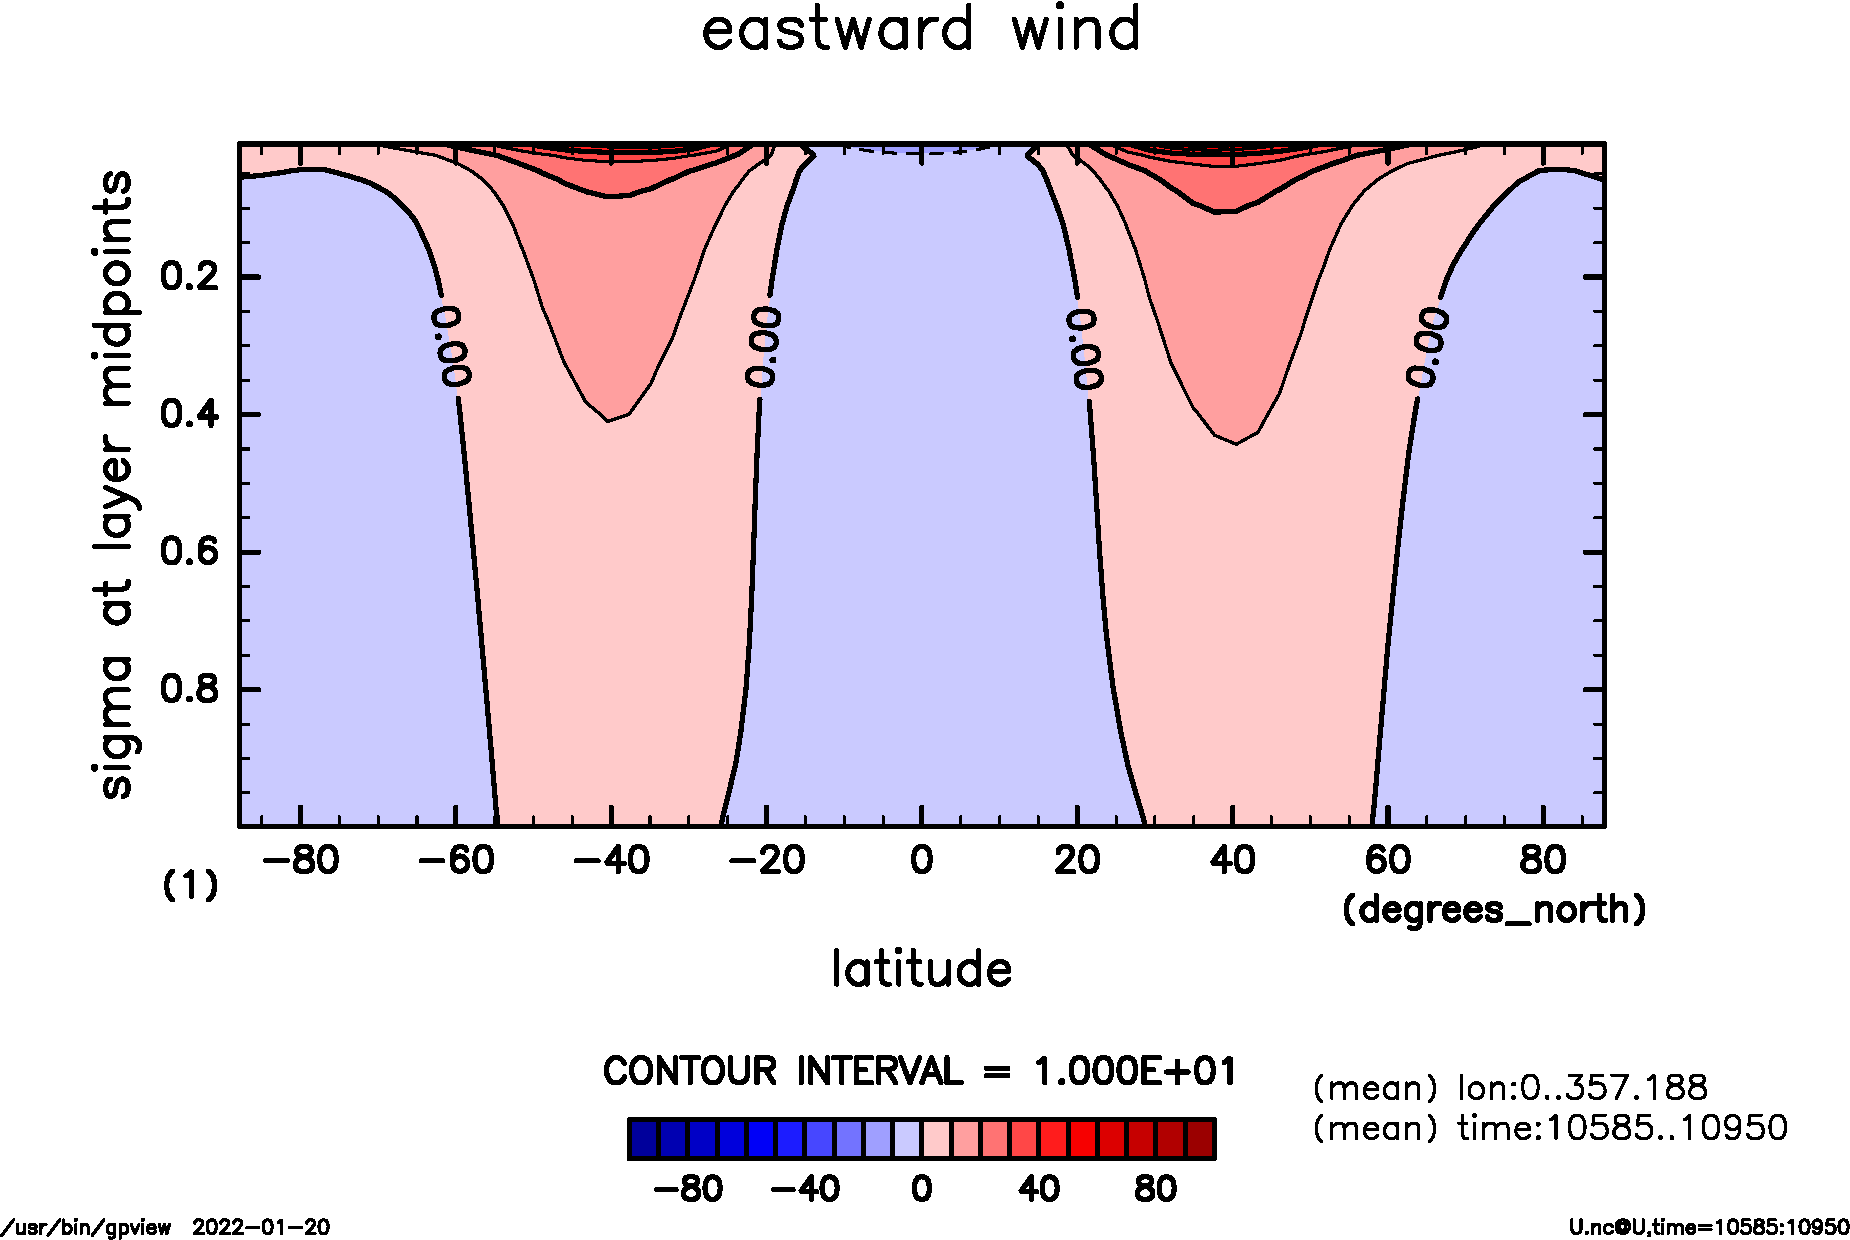
\includegraphics[width=\columnwidth]{S2000/U,time=10585:10950-crop-rotate.pdf}
		\caption{東西風}
	\end{subfigure}
	\begin{subfigure}{.4\textwidth}
		\centering
		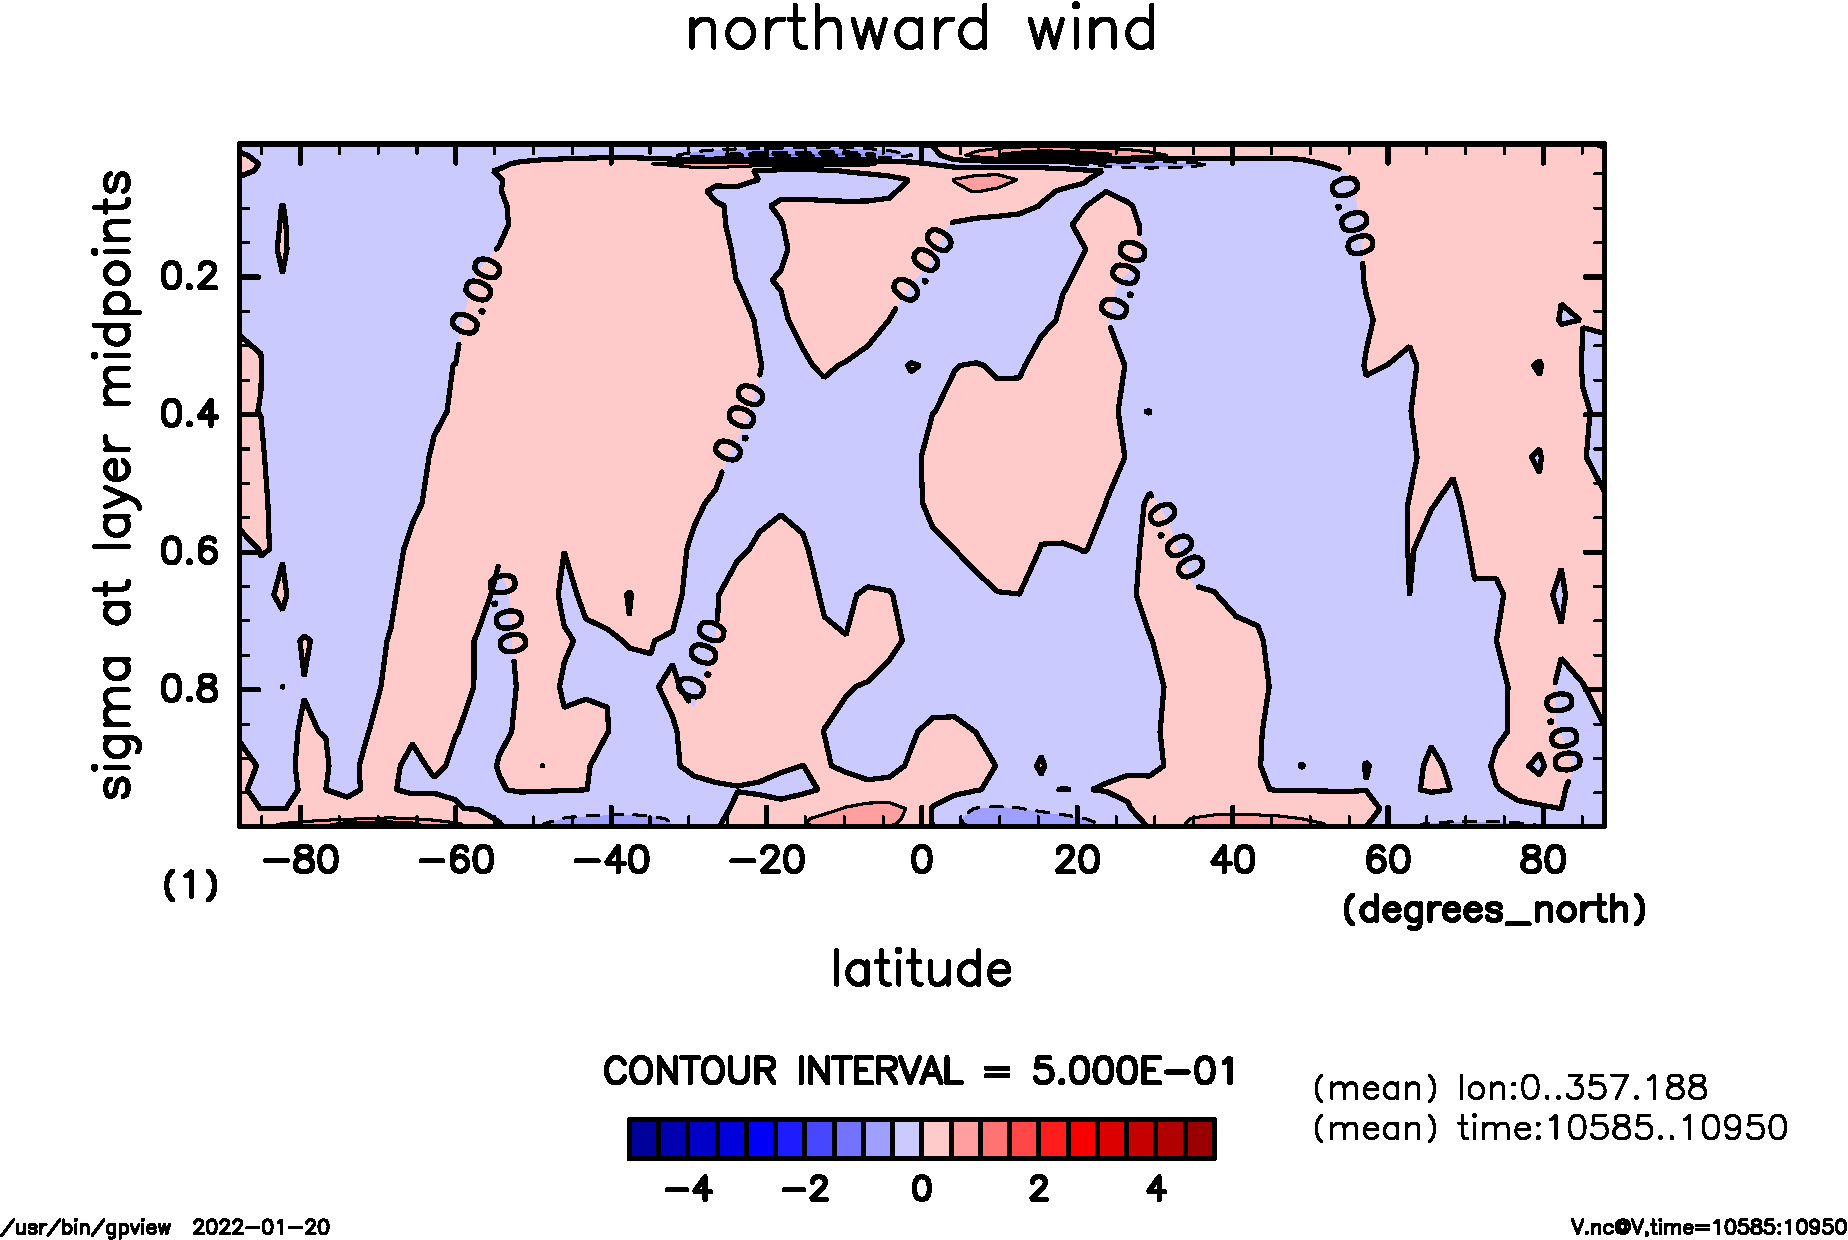
\includegraphics[width=\columnwidth]{S2000/V,time=10585:10950-crop-rotate.pdf}
		\caption{南北風}
	\end{subfigure}
	\begin{subfigure}{.4\textwidth}
		\centering
		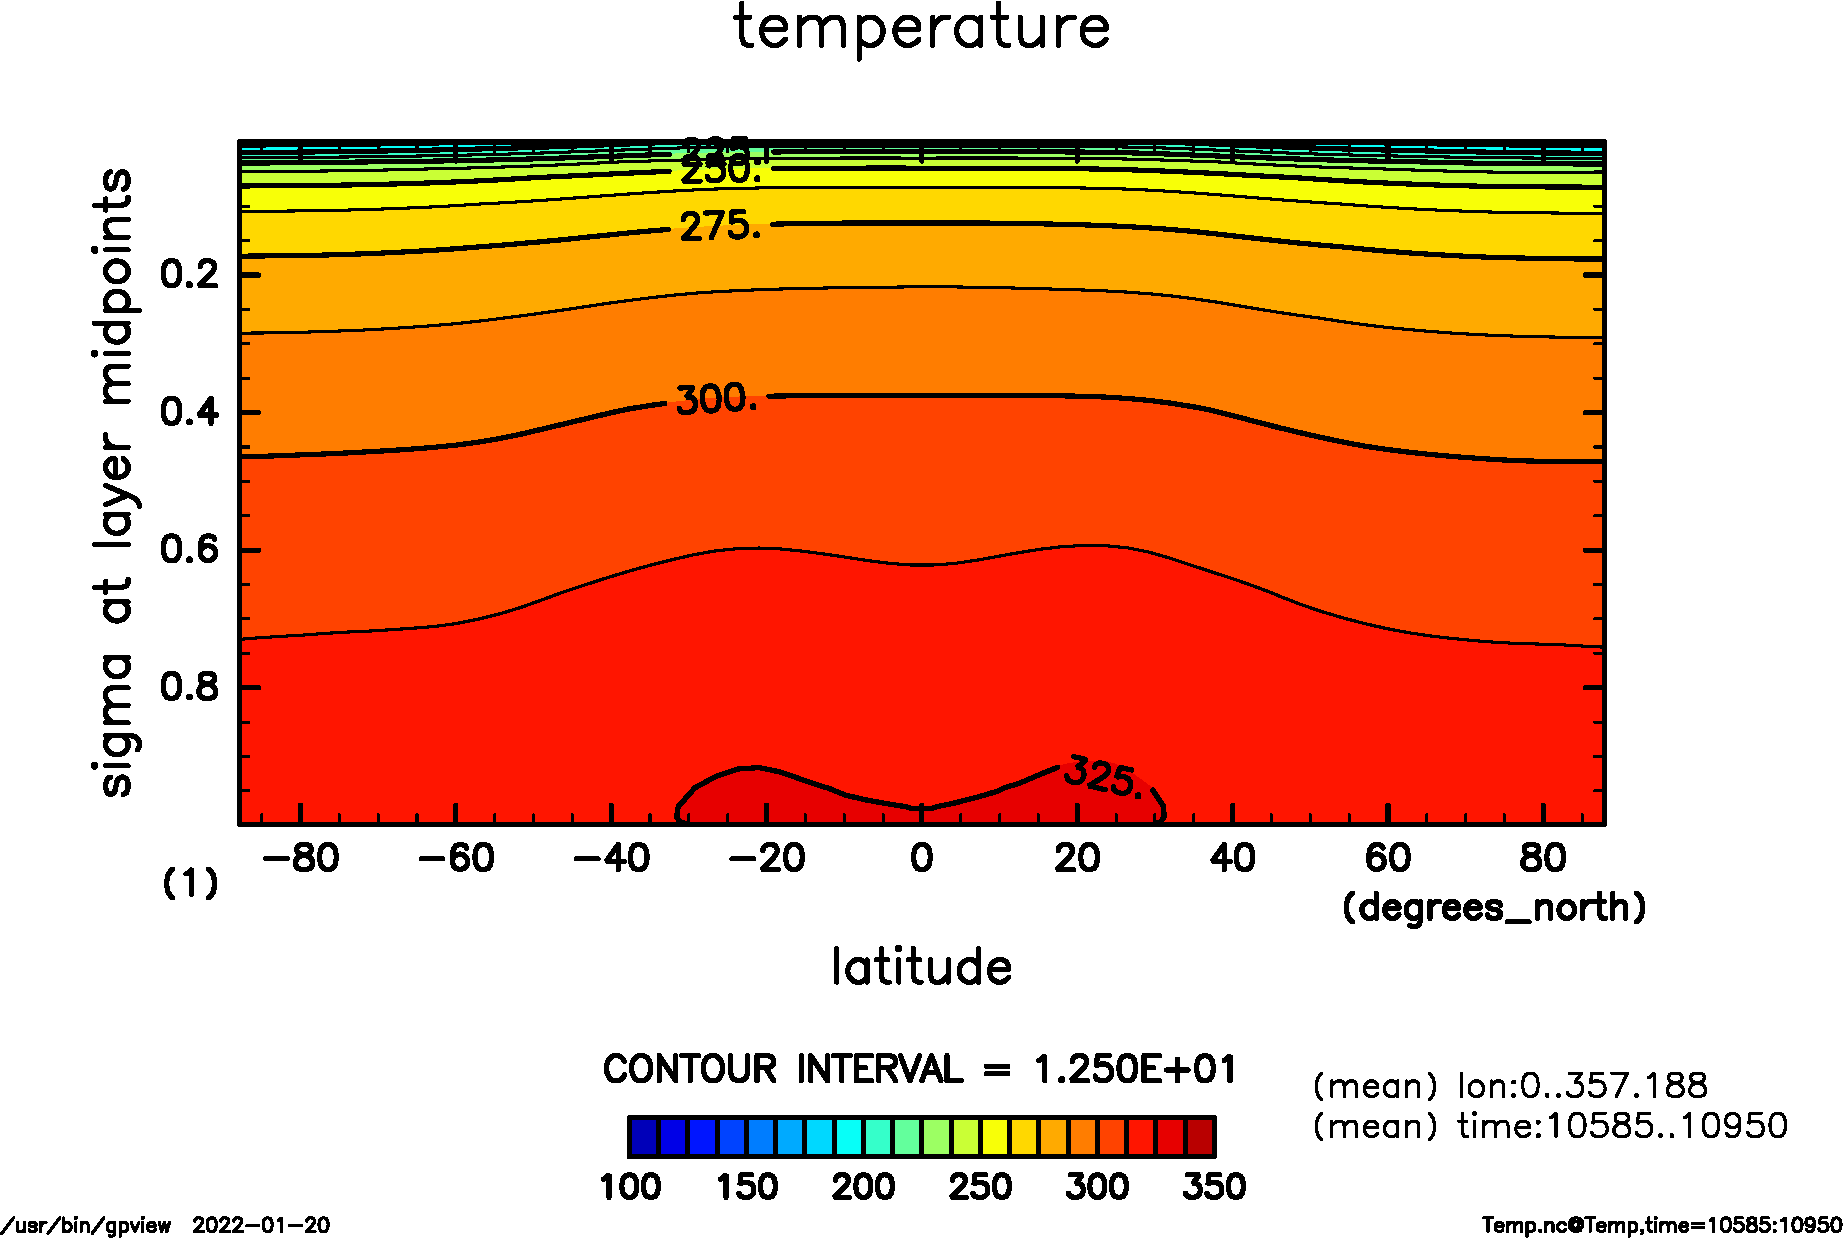
\includegraphics[width=\columnwidth]{S2000/Temp,time=10585:10950-crop-rotate.pdf}
		\caption{気温分布}
	\end{subfigure}
	\begin{subfigure}{.4\textwidth}
		\centering
		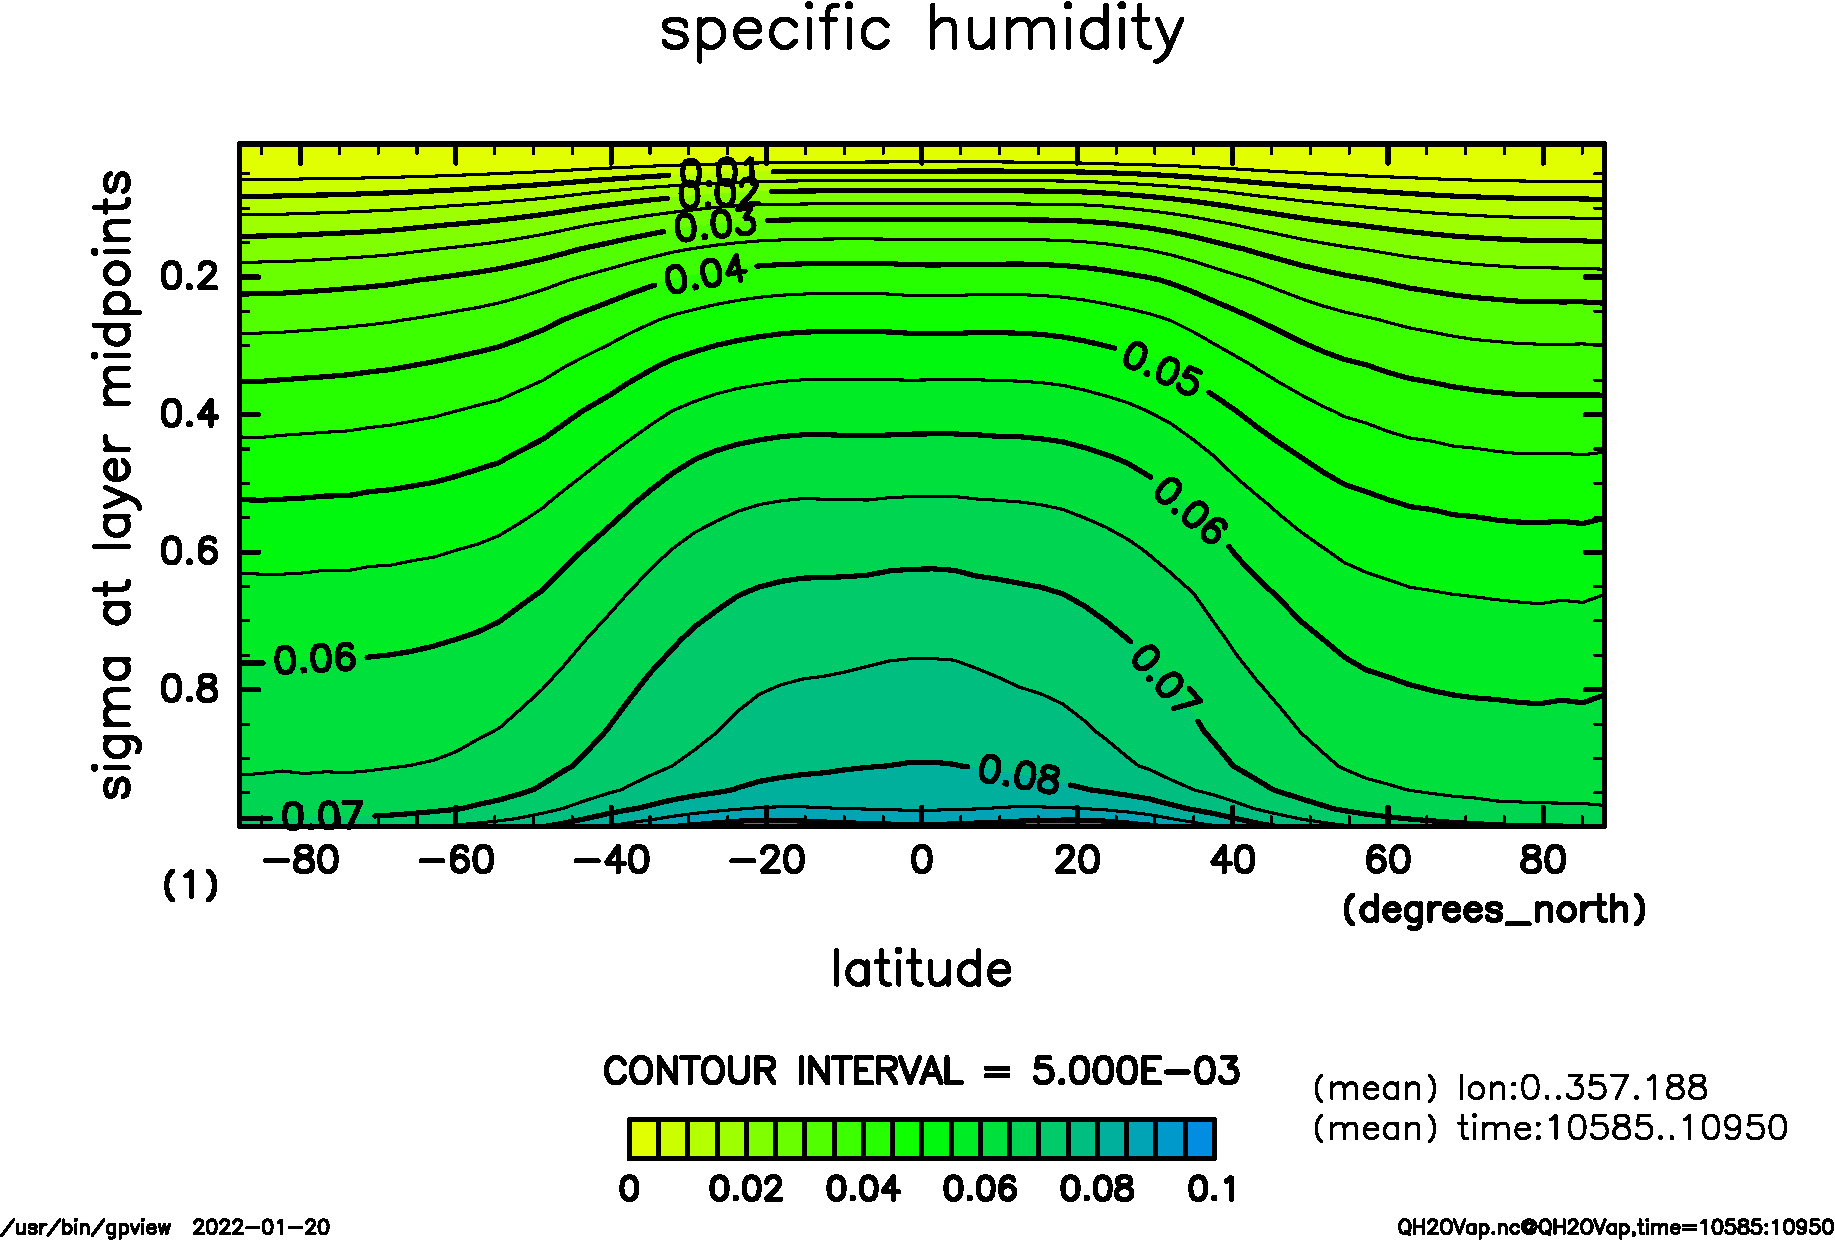
\includegraphics[width=\columnwidth]{S2000/QH2OVap,time=10585:10950-crop-rotate.pdf}
		\caption{比湿}
	\end{subfigure}
	\begin{subfigure}{.4\textwidth}
		\centering
		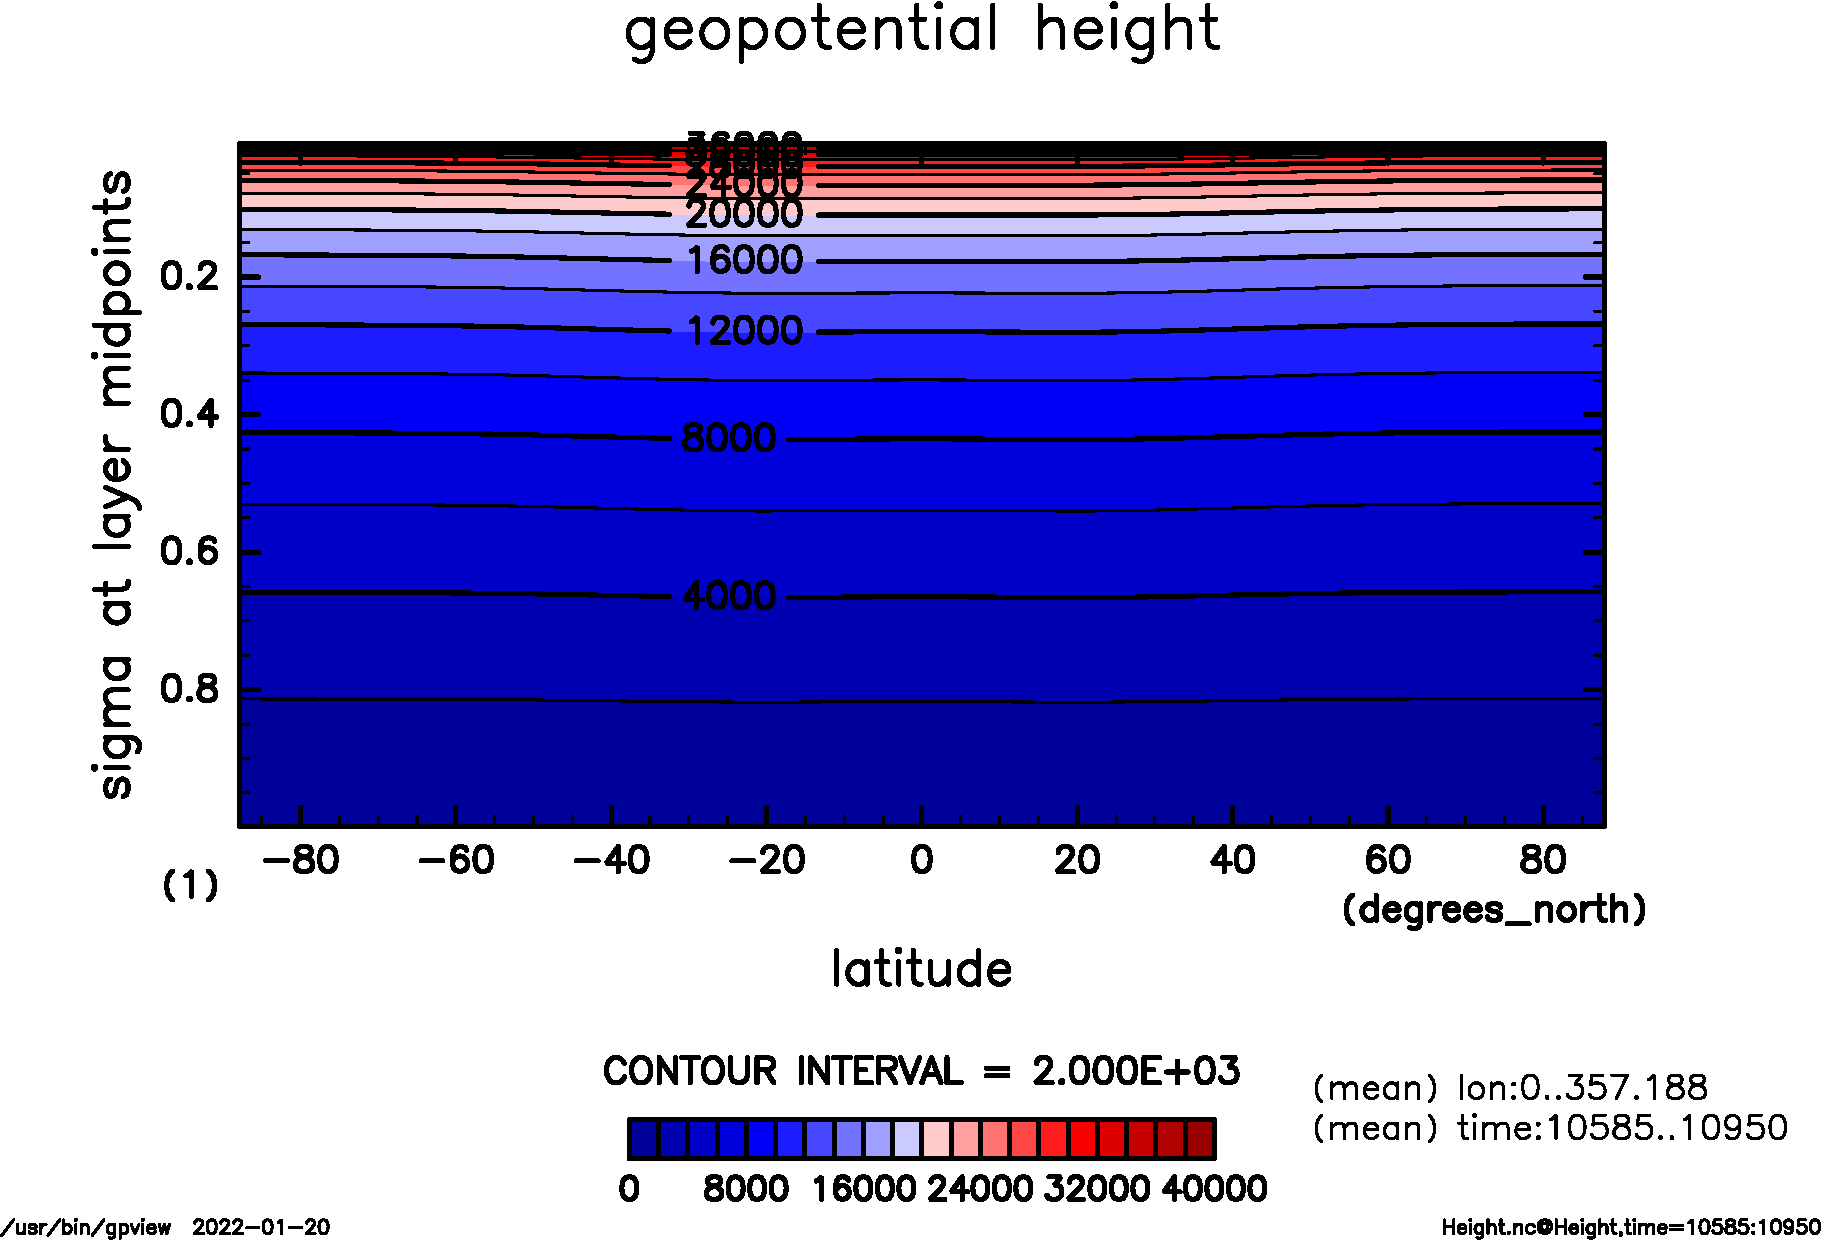
\includegraphics[width=\columnwidth]{S2000/Height,time=10585:10950-crop-rotate.pdf}
		\caption{ジオポテンシャル高度}
	\end{subfigure}
	\caption{
		\(S=2000\hmu{W/m^2}\) の結果
	}
\end{figure}

\section{??? の太陽定数依存性}

\section{南北熱輸送の太陽定数依存性}

\(\bullet'=\bullet-\bar\bullet\)、\(\bullet^*=\bullet-[\bullet]\)、
\(\bar\bullet\) は時間平均、\([\bullet]\) は東西平均

\begin{equation}
	\begin{split}
		[\overline{xv}]&=[\overline{(\bar x-x')(\bar v-v')}]\\
		&=[\overline{\bar x\bar v}+\overline{x'\bar v}+\overline{\bar xv'}+\overline{x'v'}]\\
		&=[\bar x\bar v]+[\bar{x'}\bar v]+[\bar x\bar{v'}]+[\overline{x'v'}]\\
		&=[\bar x\bar v]+[\overline{x'v'}]\\
		&=[\overline{([x]+x^*)}\overline{([v]+v^*)}]+[\overline{x'v'}]\\
		&=[([\bar x]+\bar{x^*})([\bar v]+\bar{v^*})]+[\overline{x'v'}]\\
		&=[[\bar x][\bar v]]+[\bar{x^*}[\bar v]]+[[\bar x]\bar{v^*}]+[\bar{x^*}\bar{v^*}]+[\overline{x'v'}]\\
		&=[\bar x][\bar v]+[\bar{x^*}\bar{v^*}]+[\overline{x'v'}]
	\end{split}
\end{equation}

\end{document}
